% Appendix Template

\chapter{FFT plots} % Main appendix title

\label{fft_results} % Change X to a consecutive letter; for referencing this appendix elsewhere, use \ref{AppendixX}

\fancyhead[RE, LO]{\emph{FFT plots}} % Change X to a consecutive letter; this is for the header on each page - perhaps a shortened title

\begin{figure}[ht]
	\centering
	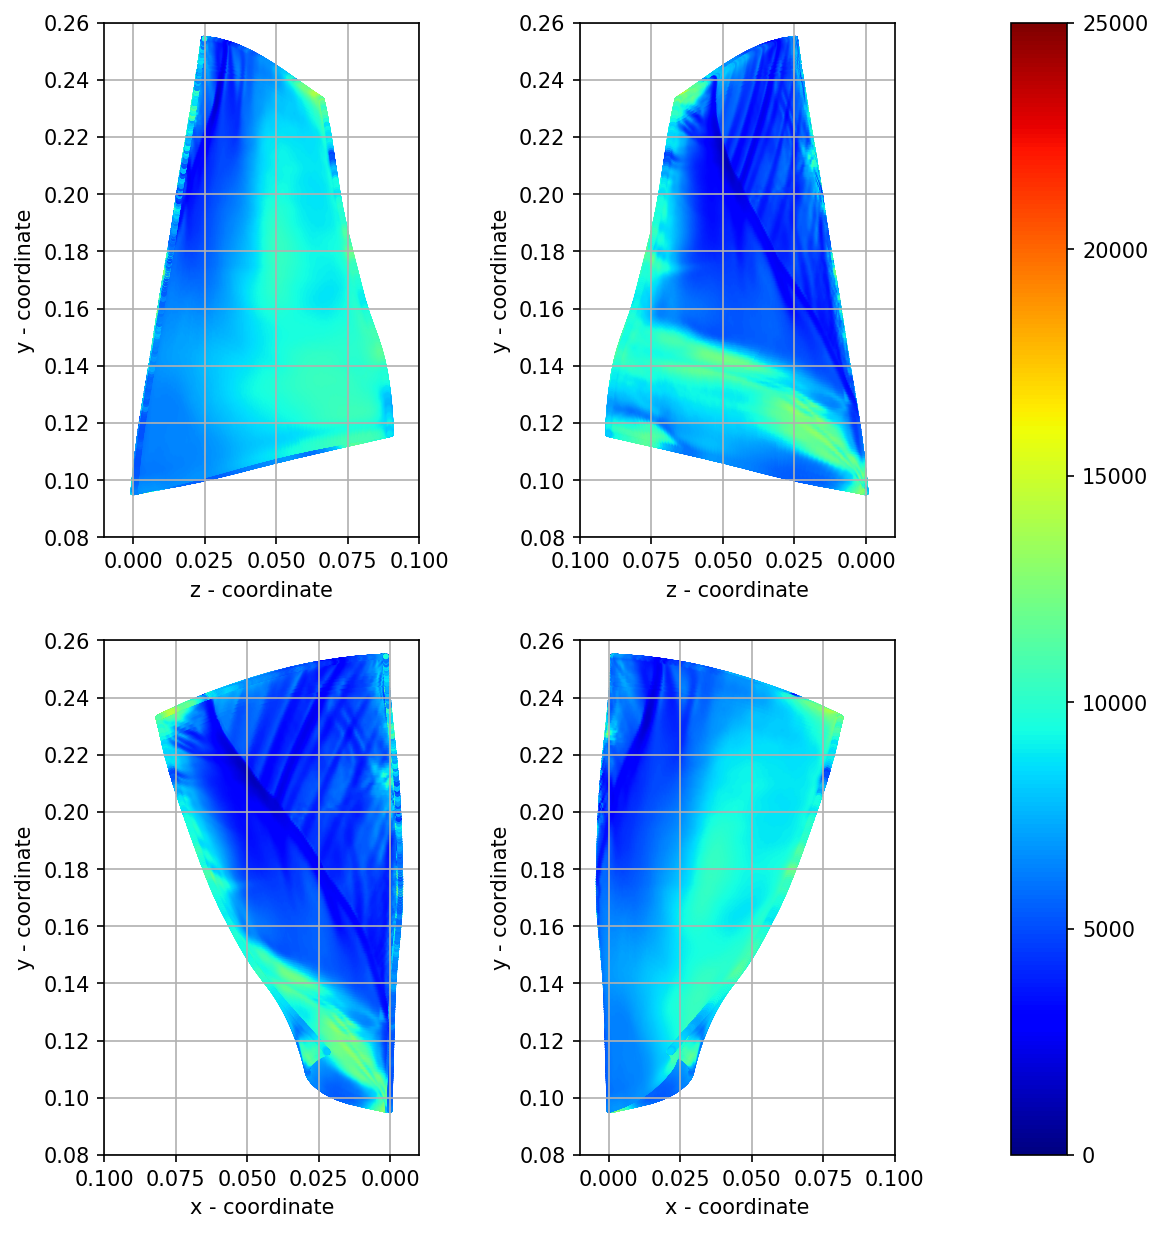
\includegraphics[width=0.9\textwidth]{Figures/blade-awf.png}
    \caption{Blade surface amplitude weighted average frequency [dB]} \label{blade-awaf}
\end{figure}	

\begin{figure}[ht]
	\centering
	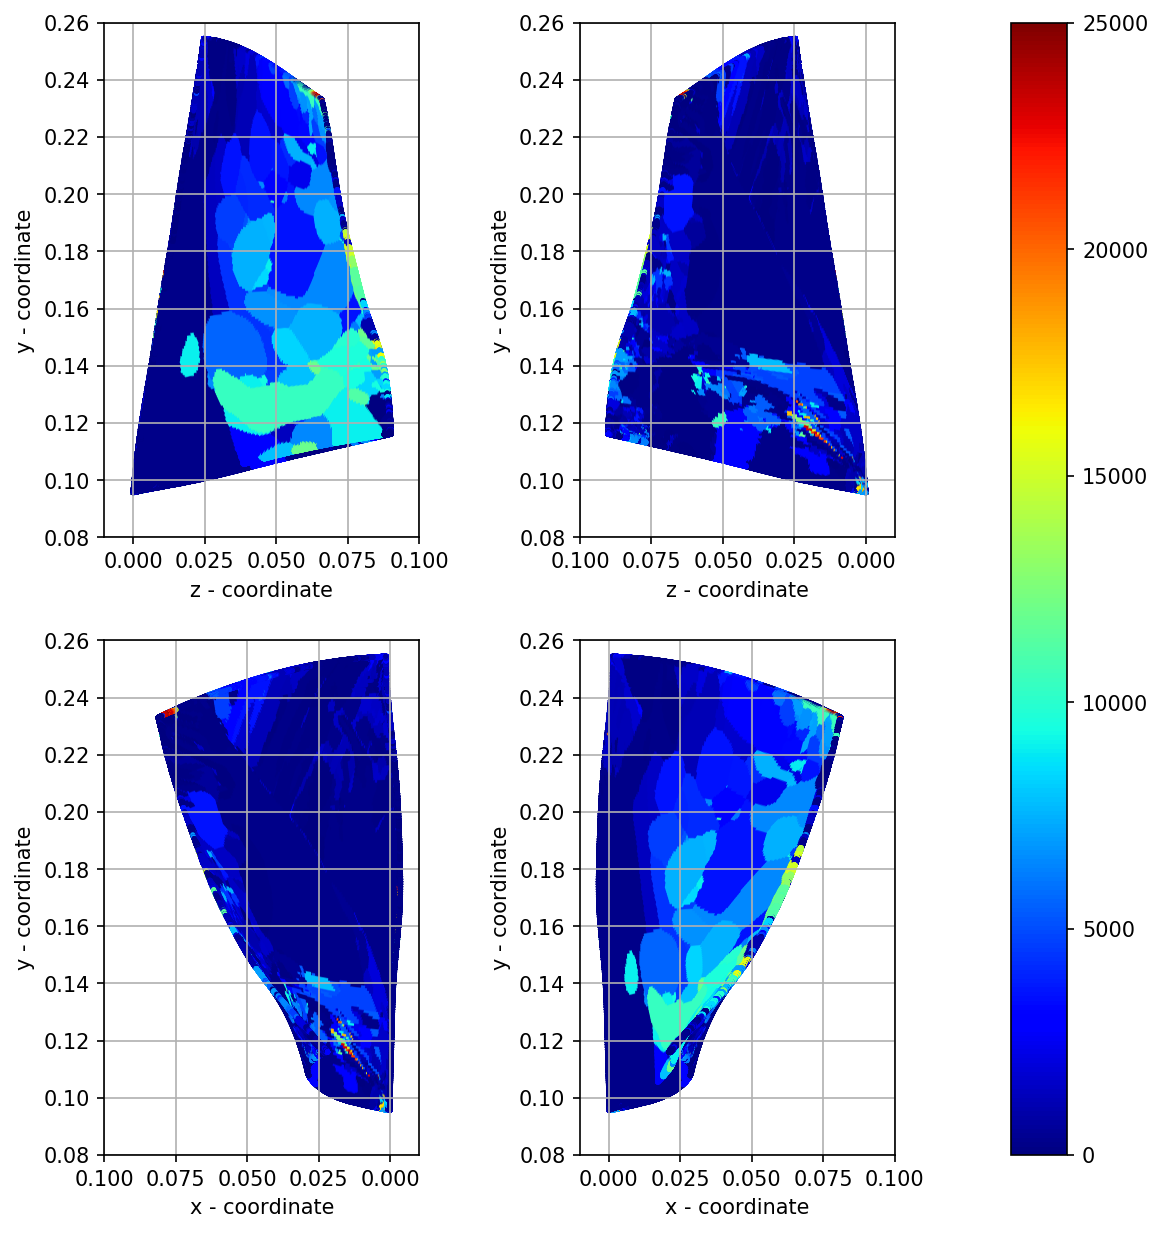
\includegraphics[width=0.9\textwidth]{Figures/blade-peak-freq.png}
	\caption{Blade surface frequency of peak amplitude[Hz]} \label{blade-peak-freq}
\end{figure}

\begin{figure}[ht]
	\centering
	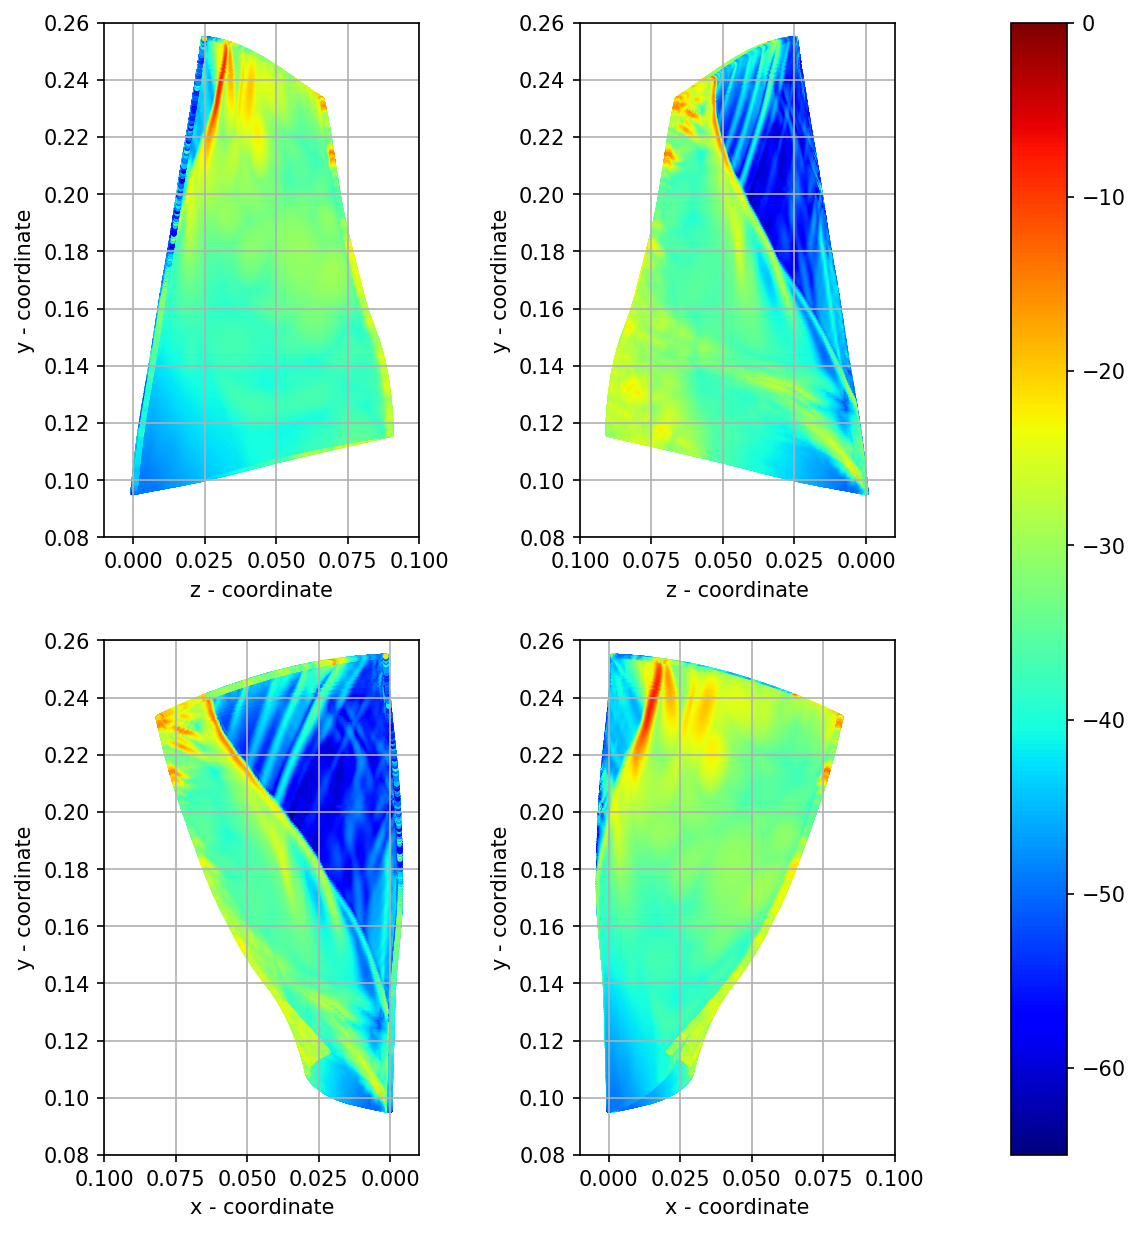
\includegraphics[width=0.9\textwidth]{Figures/blade-peak-mag.png}
	\caption{Blade surface peak amplitude [dB]} \label{blade-peak-mag}
\end{figure}

%int-01
\begin{figure}[ht]
  \centering
  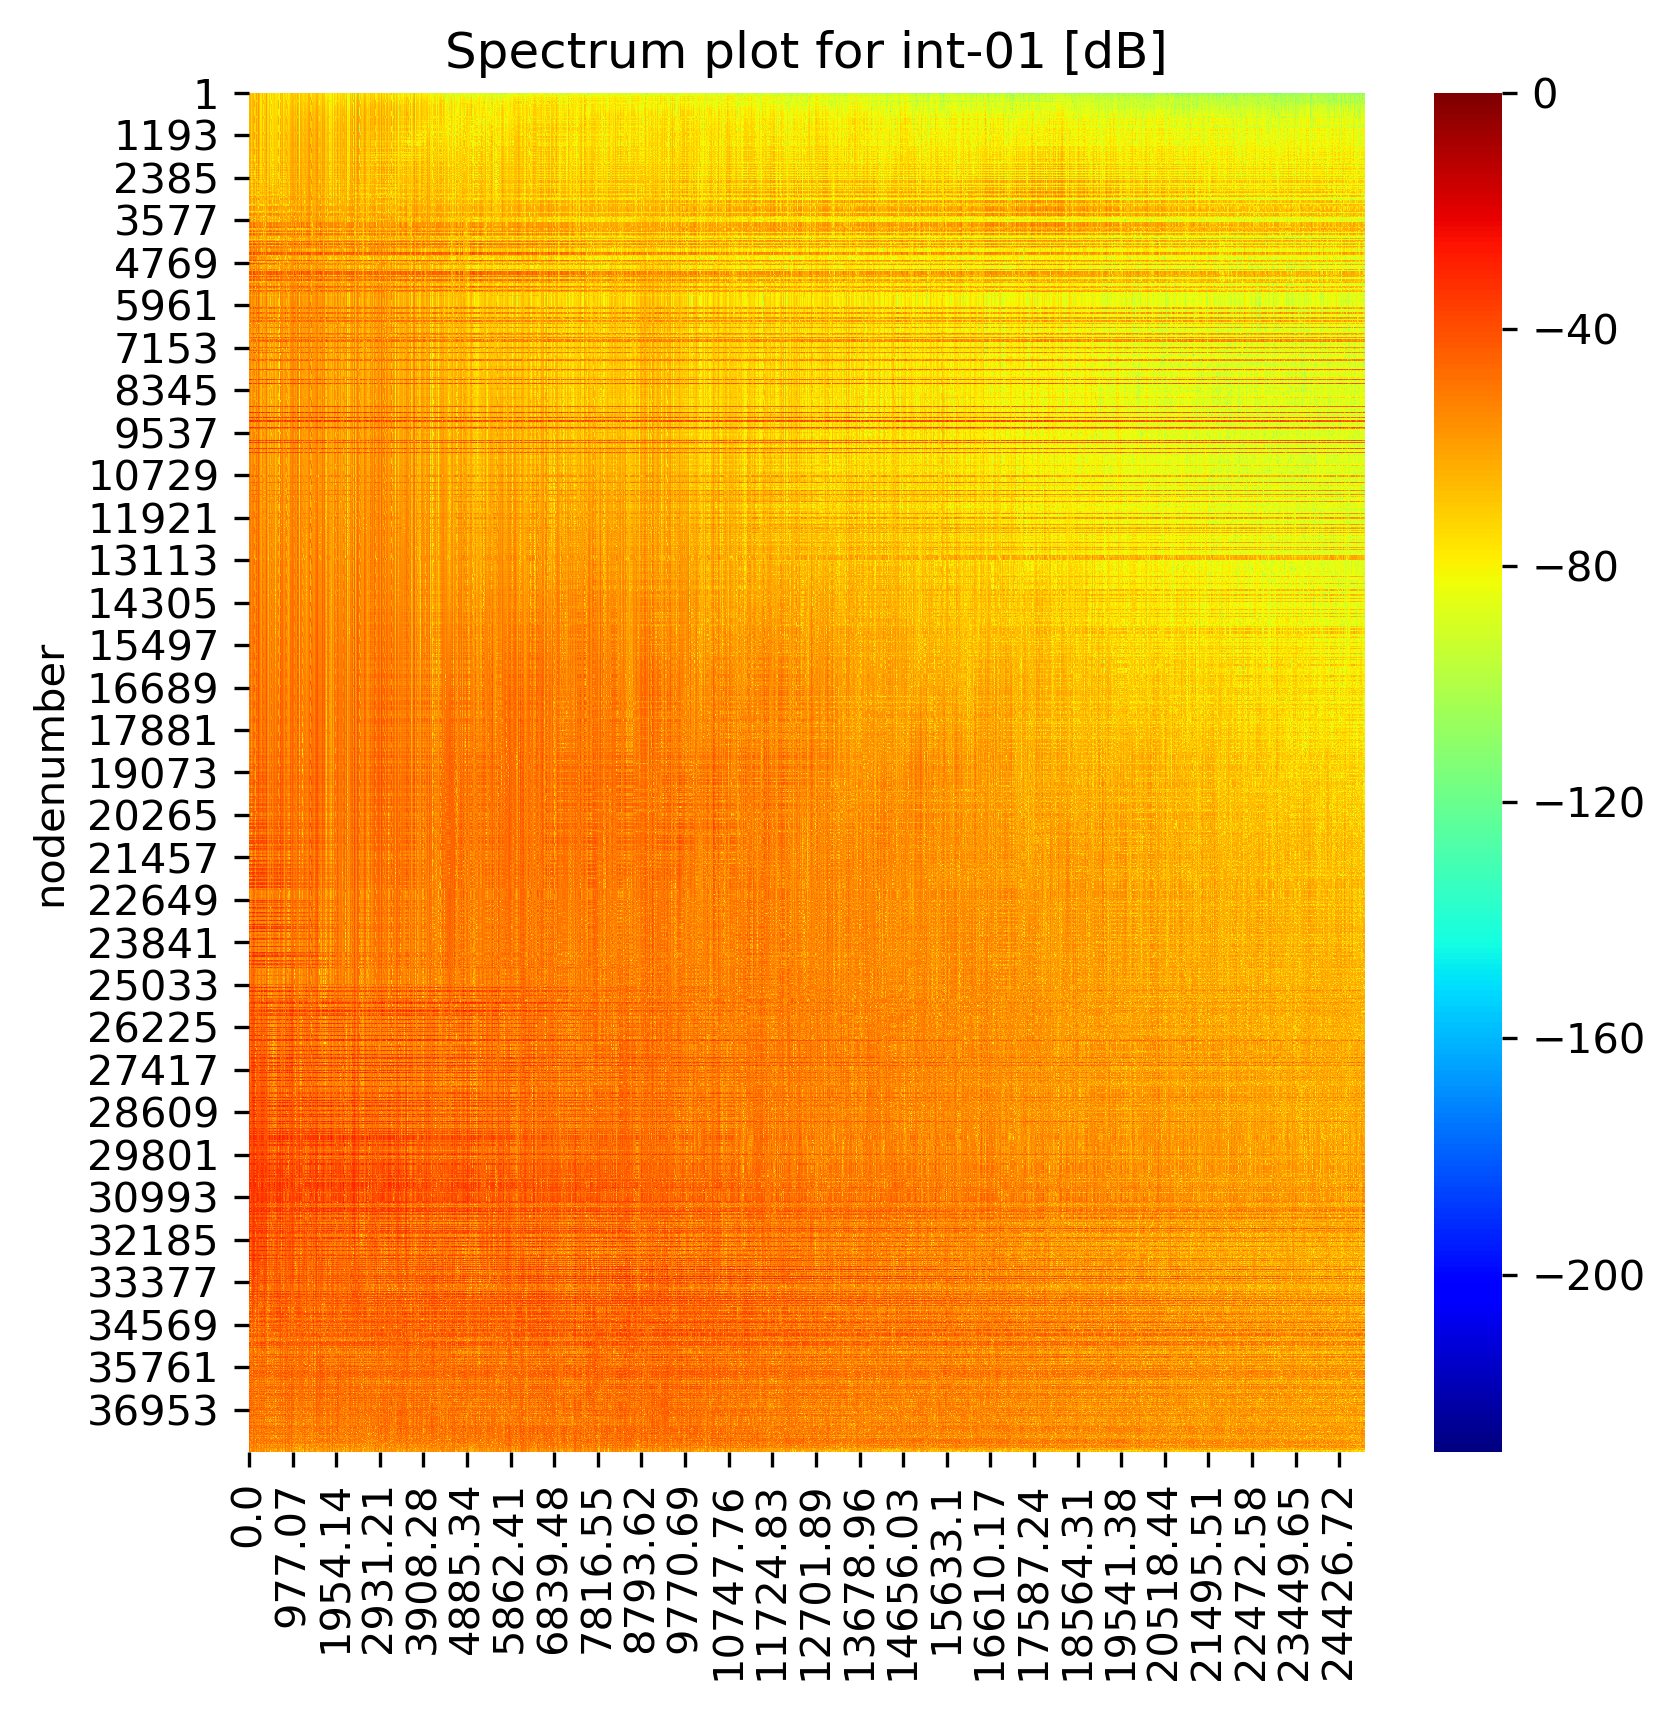
\includegraphics[width=0.75\textwidth]{Figures/int-01_spectrum.png}
  \caption{Spectrum plot at int-01 mark} \label{int-01-spectrum}
  
  \vspace*{\floatsep}% https://tex.stackexchange.com/q/26521/5764

  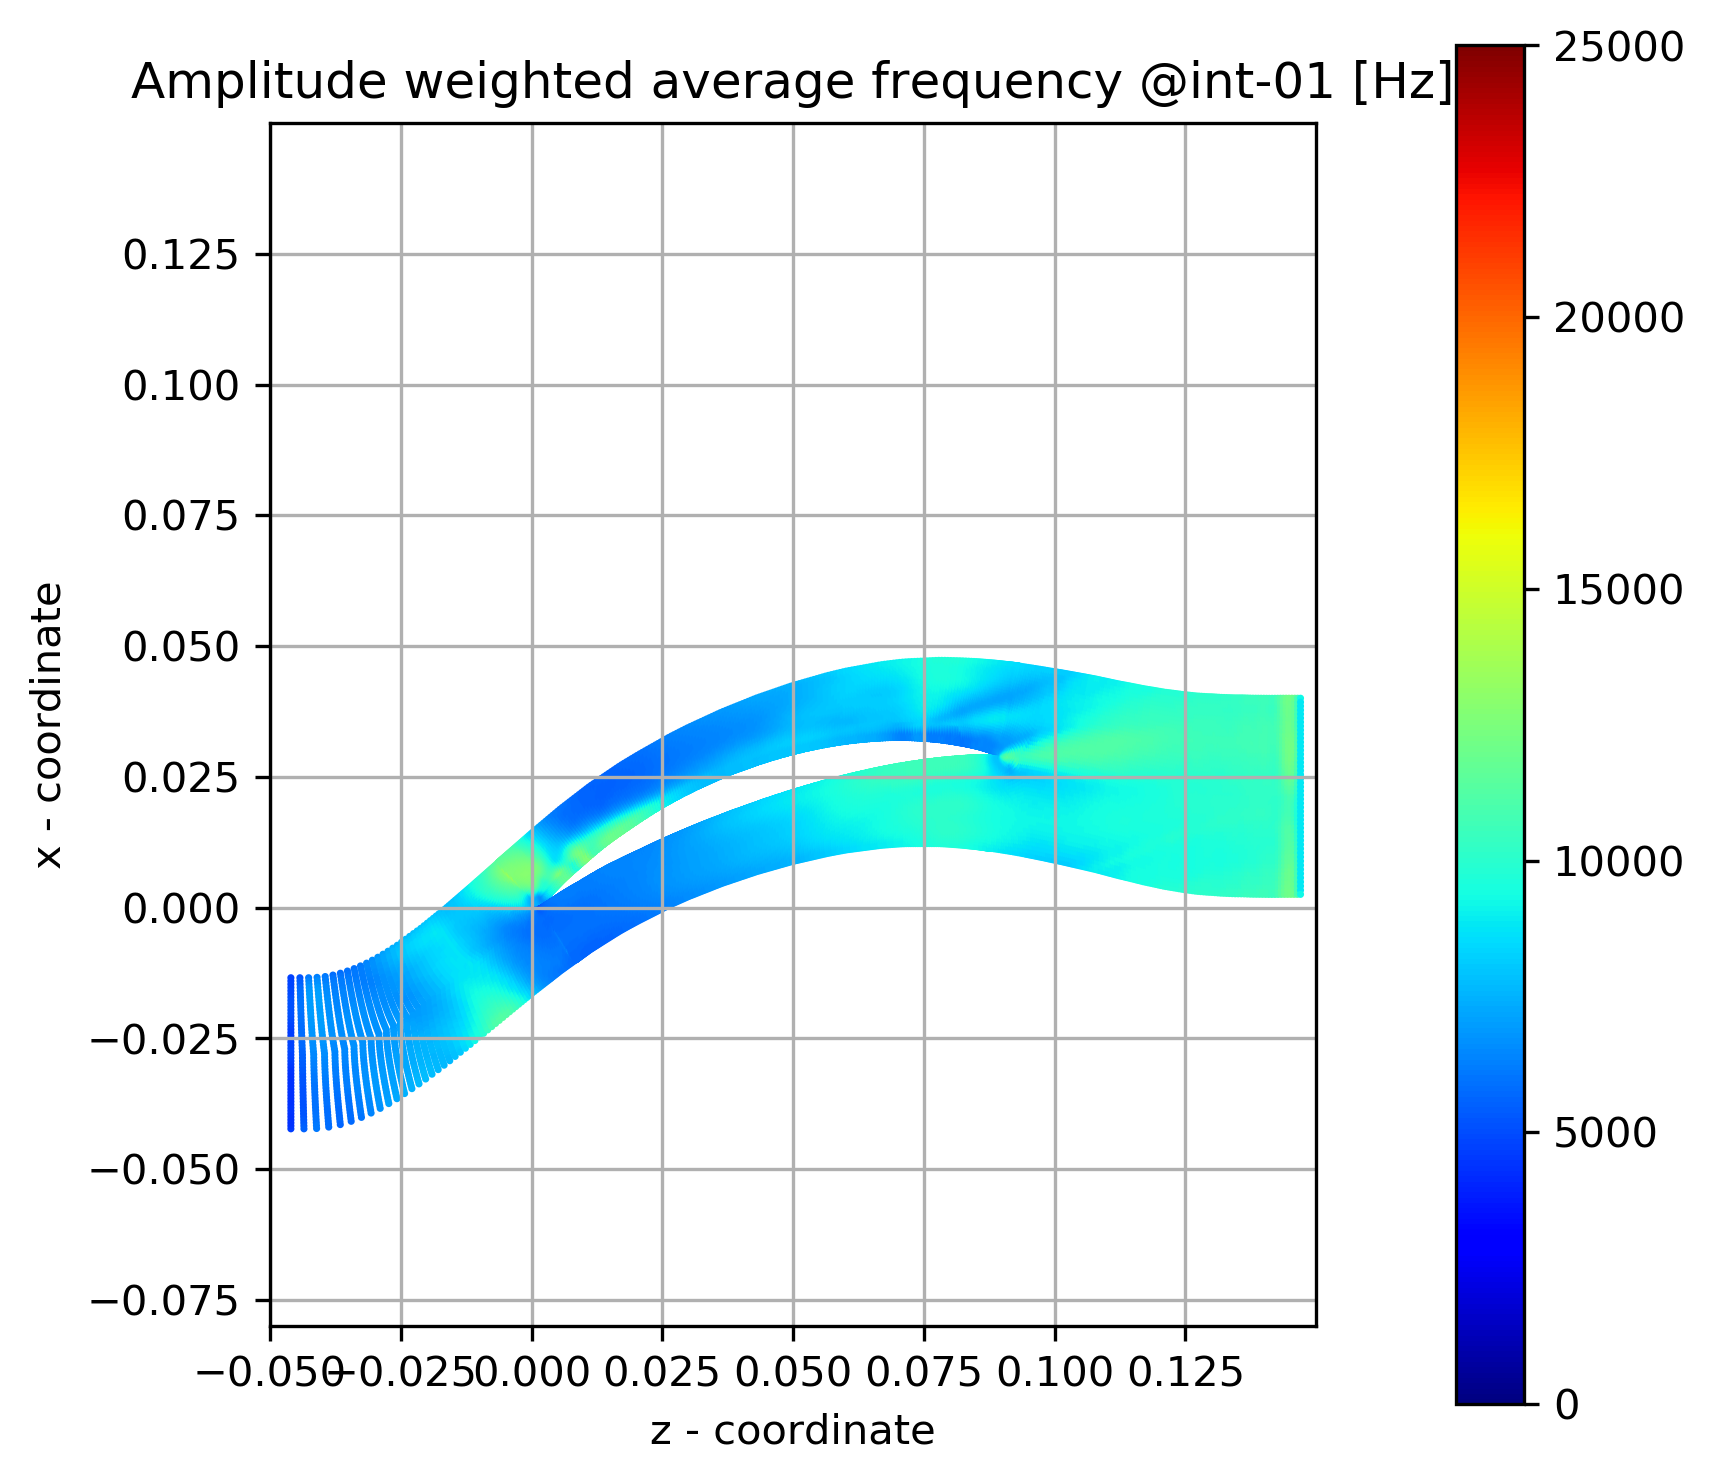
\includegraphics[width=0.75\textwidth]{Figures/int-01-awaf.png}
  \caption{Amplitude weighted average frequency at int-01 mark} \label{int-01-awaf}
\end{figure}
%int-01
\begin{figure}[ht]
  \centering
  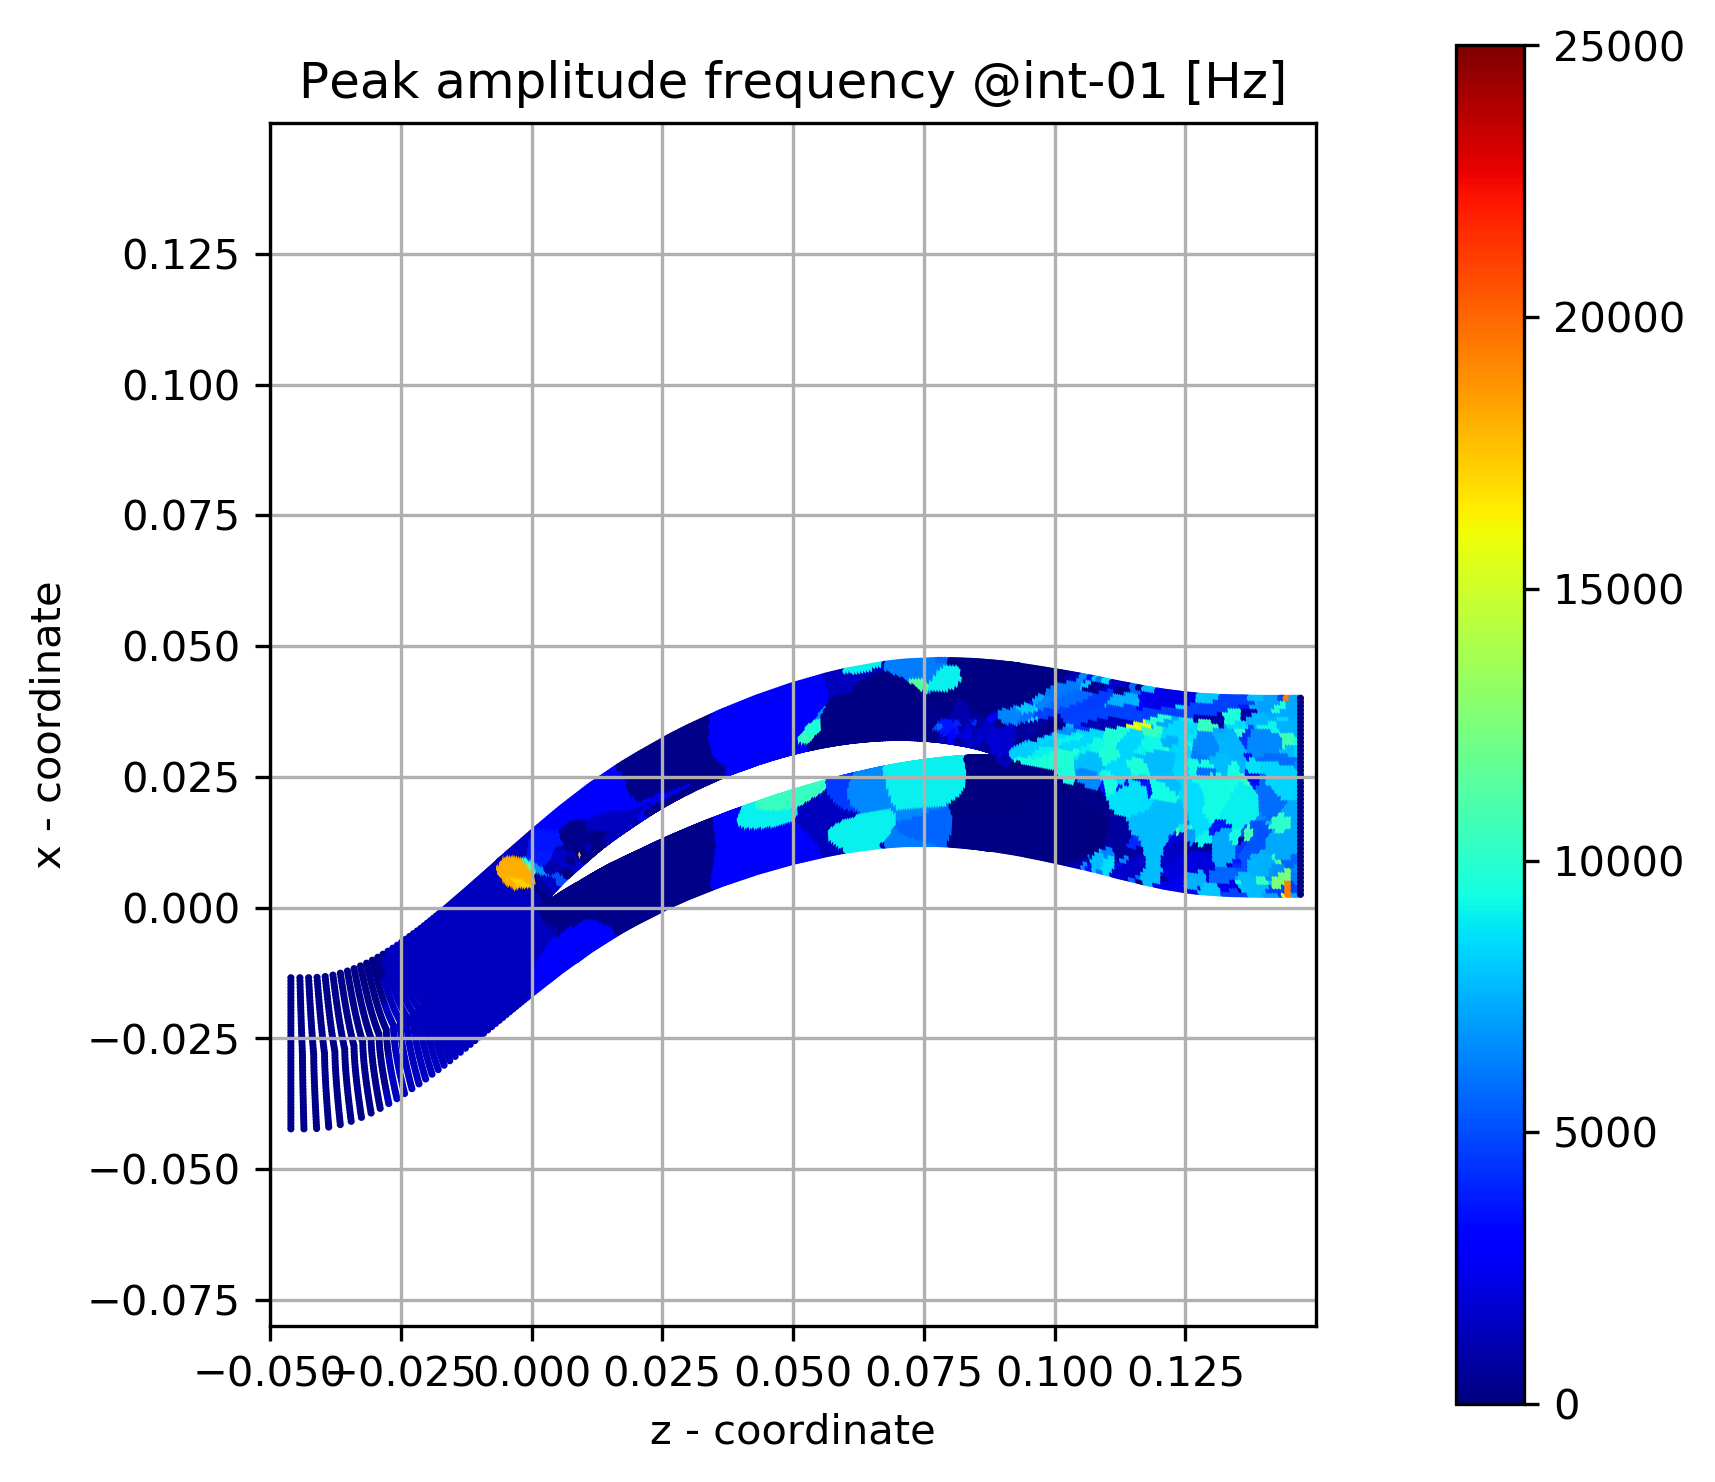
\includegraphics[width=0.75\textwidth]{Figures/int-01-peak-freq.png}
  \caption{Peak amplitude frequency int-01 mark} \label{int-01-peak-freq}
  
  \vspace*{\floatsep}% https://tex.stackexchange.com/q/26521/5764

  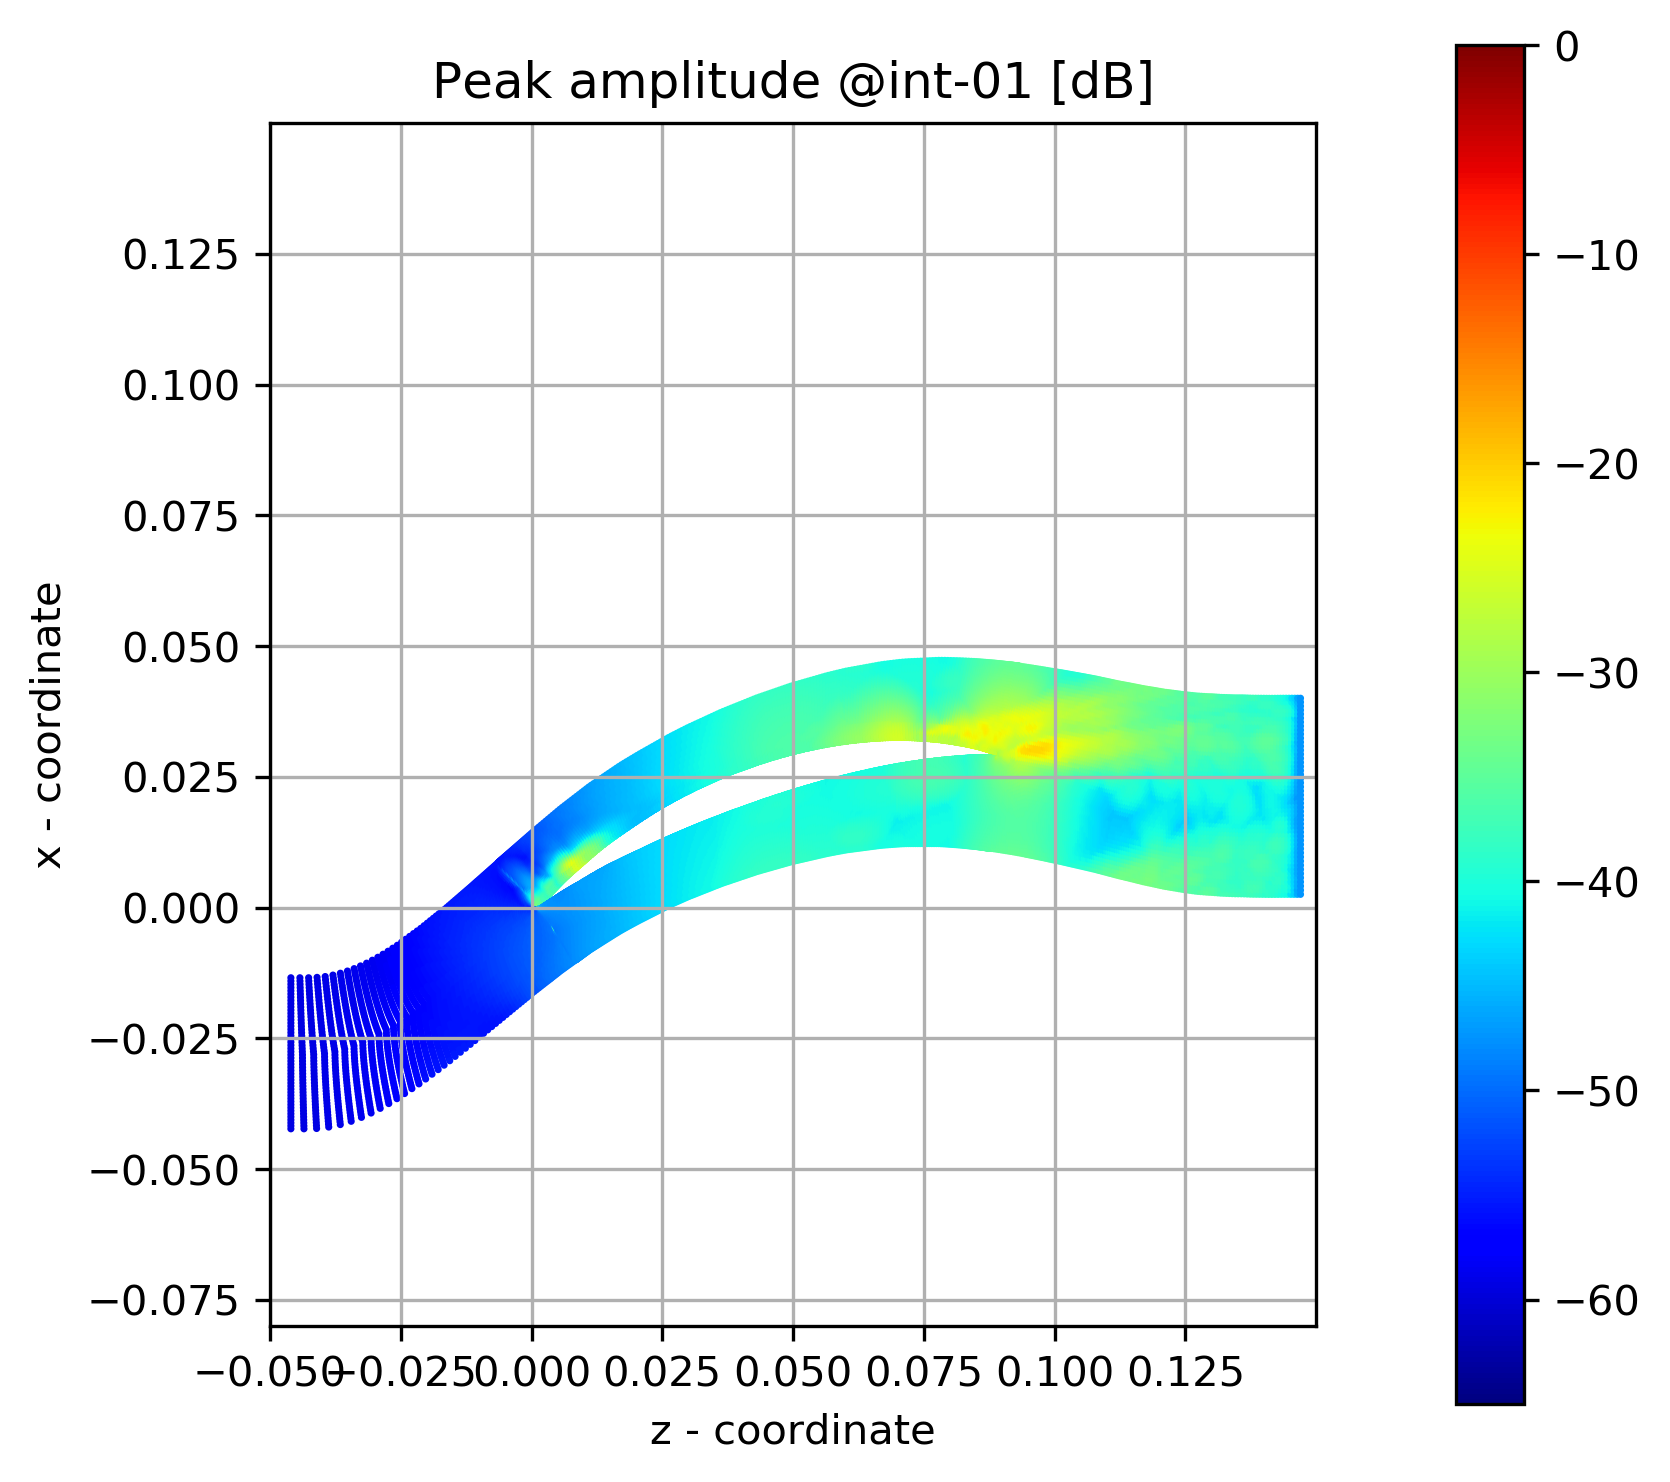
\includegraphics[width=0.75\textwidth]{Figures/int-01-peak-mag.png}
  \caption{Peak magnitude at int-01 mark} \label{int-01-peak-mag}
\end{figure}

%int-02
\begin{figure}[ht]
  \centering
  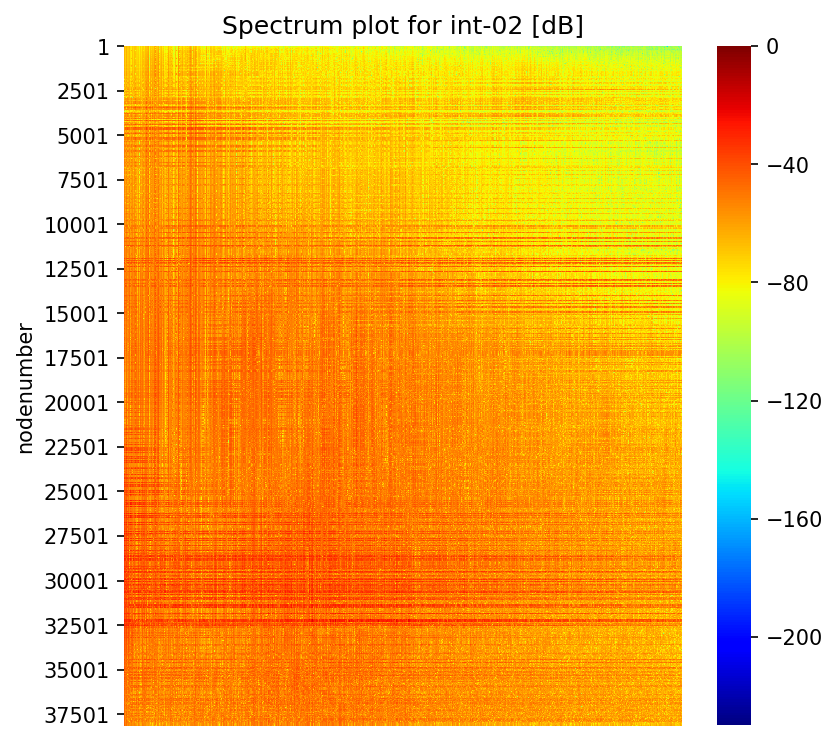
\includegraphics[width=0.75\textwidth]{Figures/int-02_spectrum.png}
  \caption{Spectrum plot at int-02 mark} \label{int-02-spectrum}
  
  \vspace*{\floatsep}% https://tex.stackexchange.com/q/26521/5764

  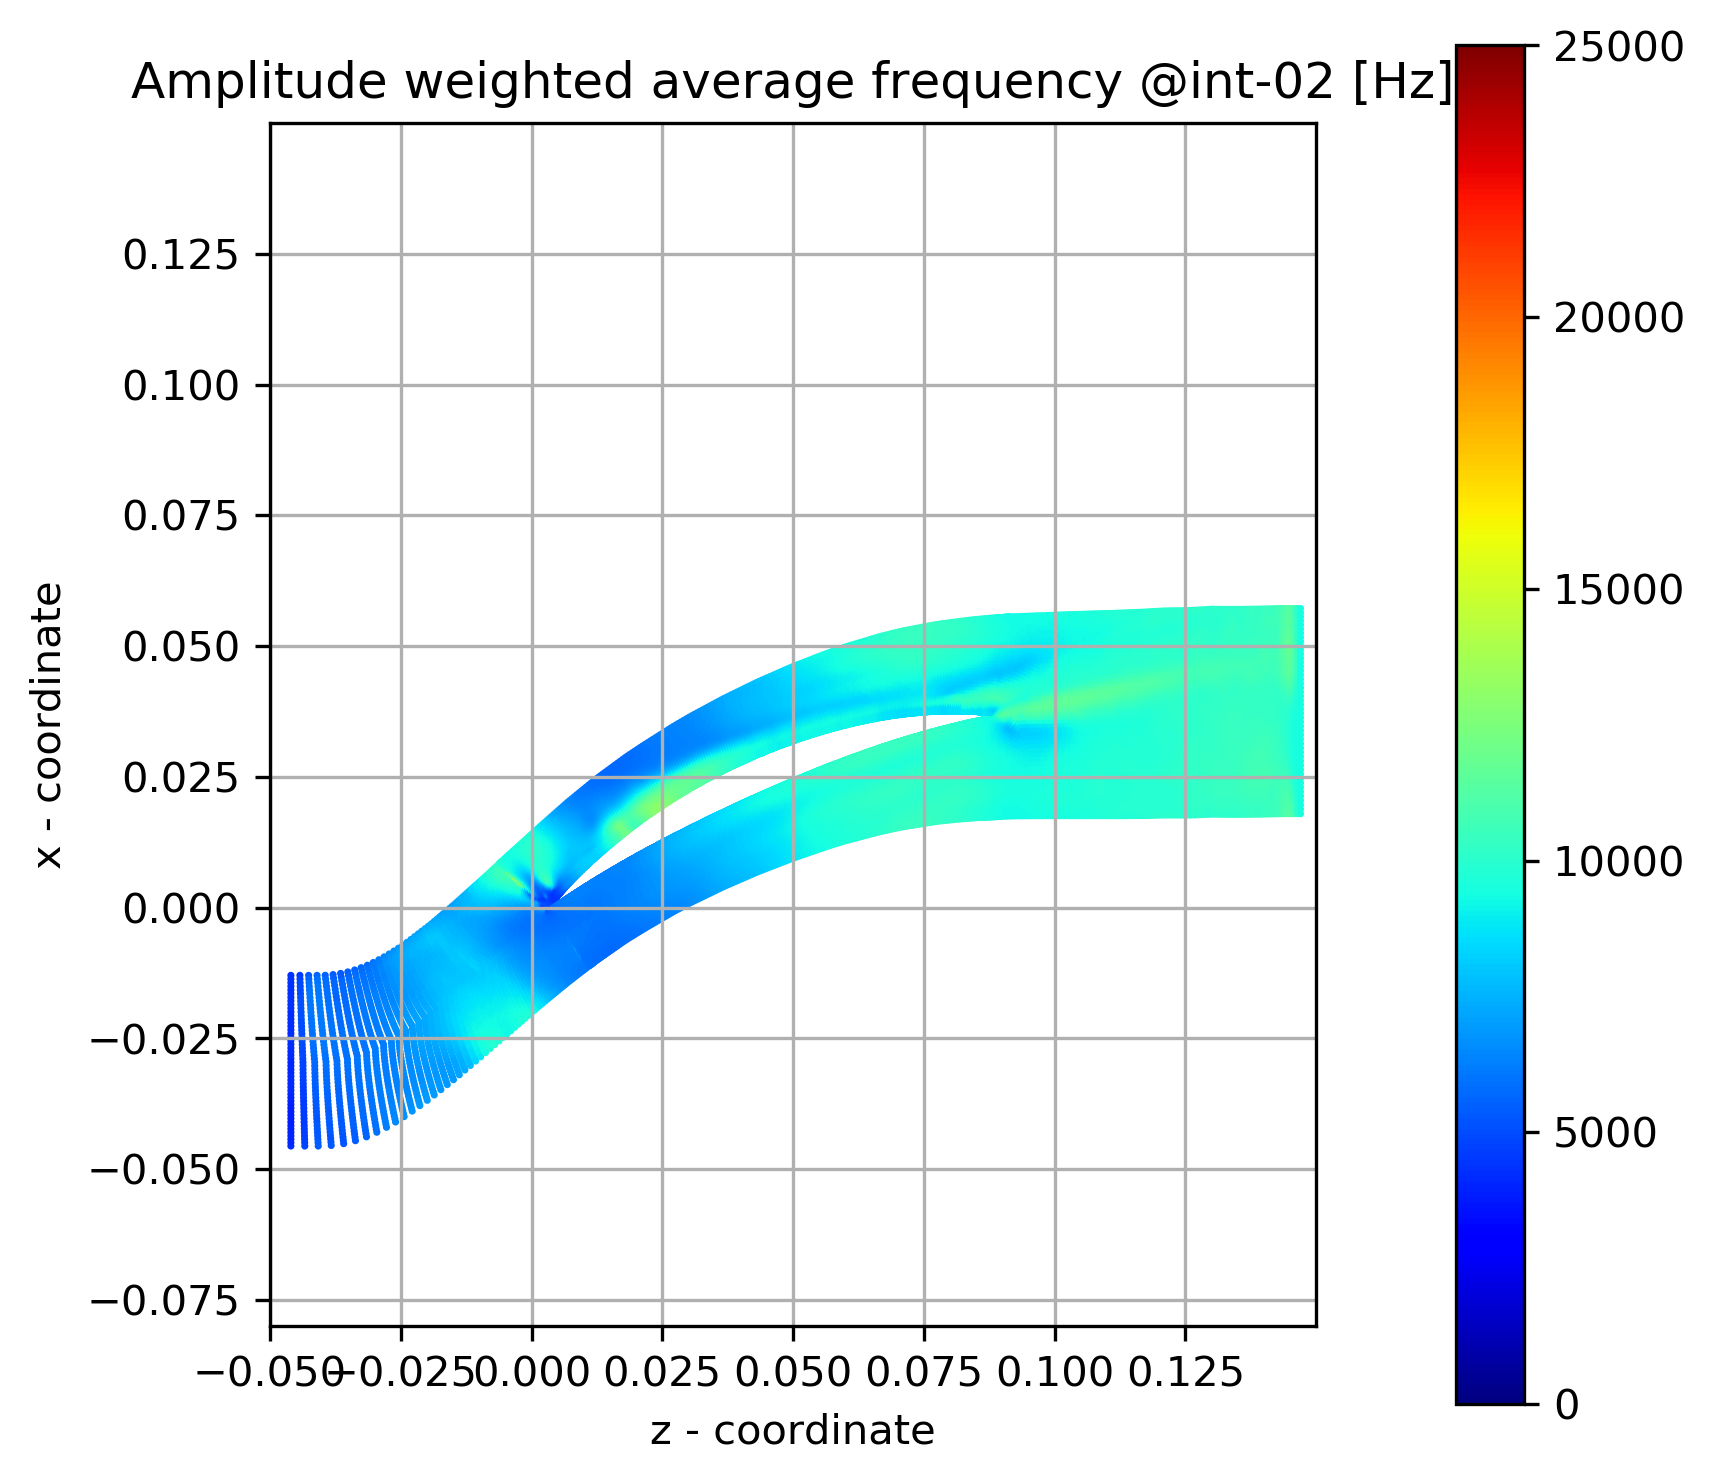
\includegraphics[width=0.75\textwidth]{Figures/int-02-awaf.png}
  \caption{Amplitude weighted average frequency at int-02 mark} \label{int-02-awaf}
\end{figure}
%int-02
\begin{figure}[ht]
  \centering
  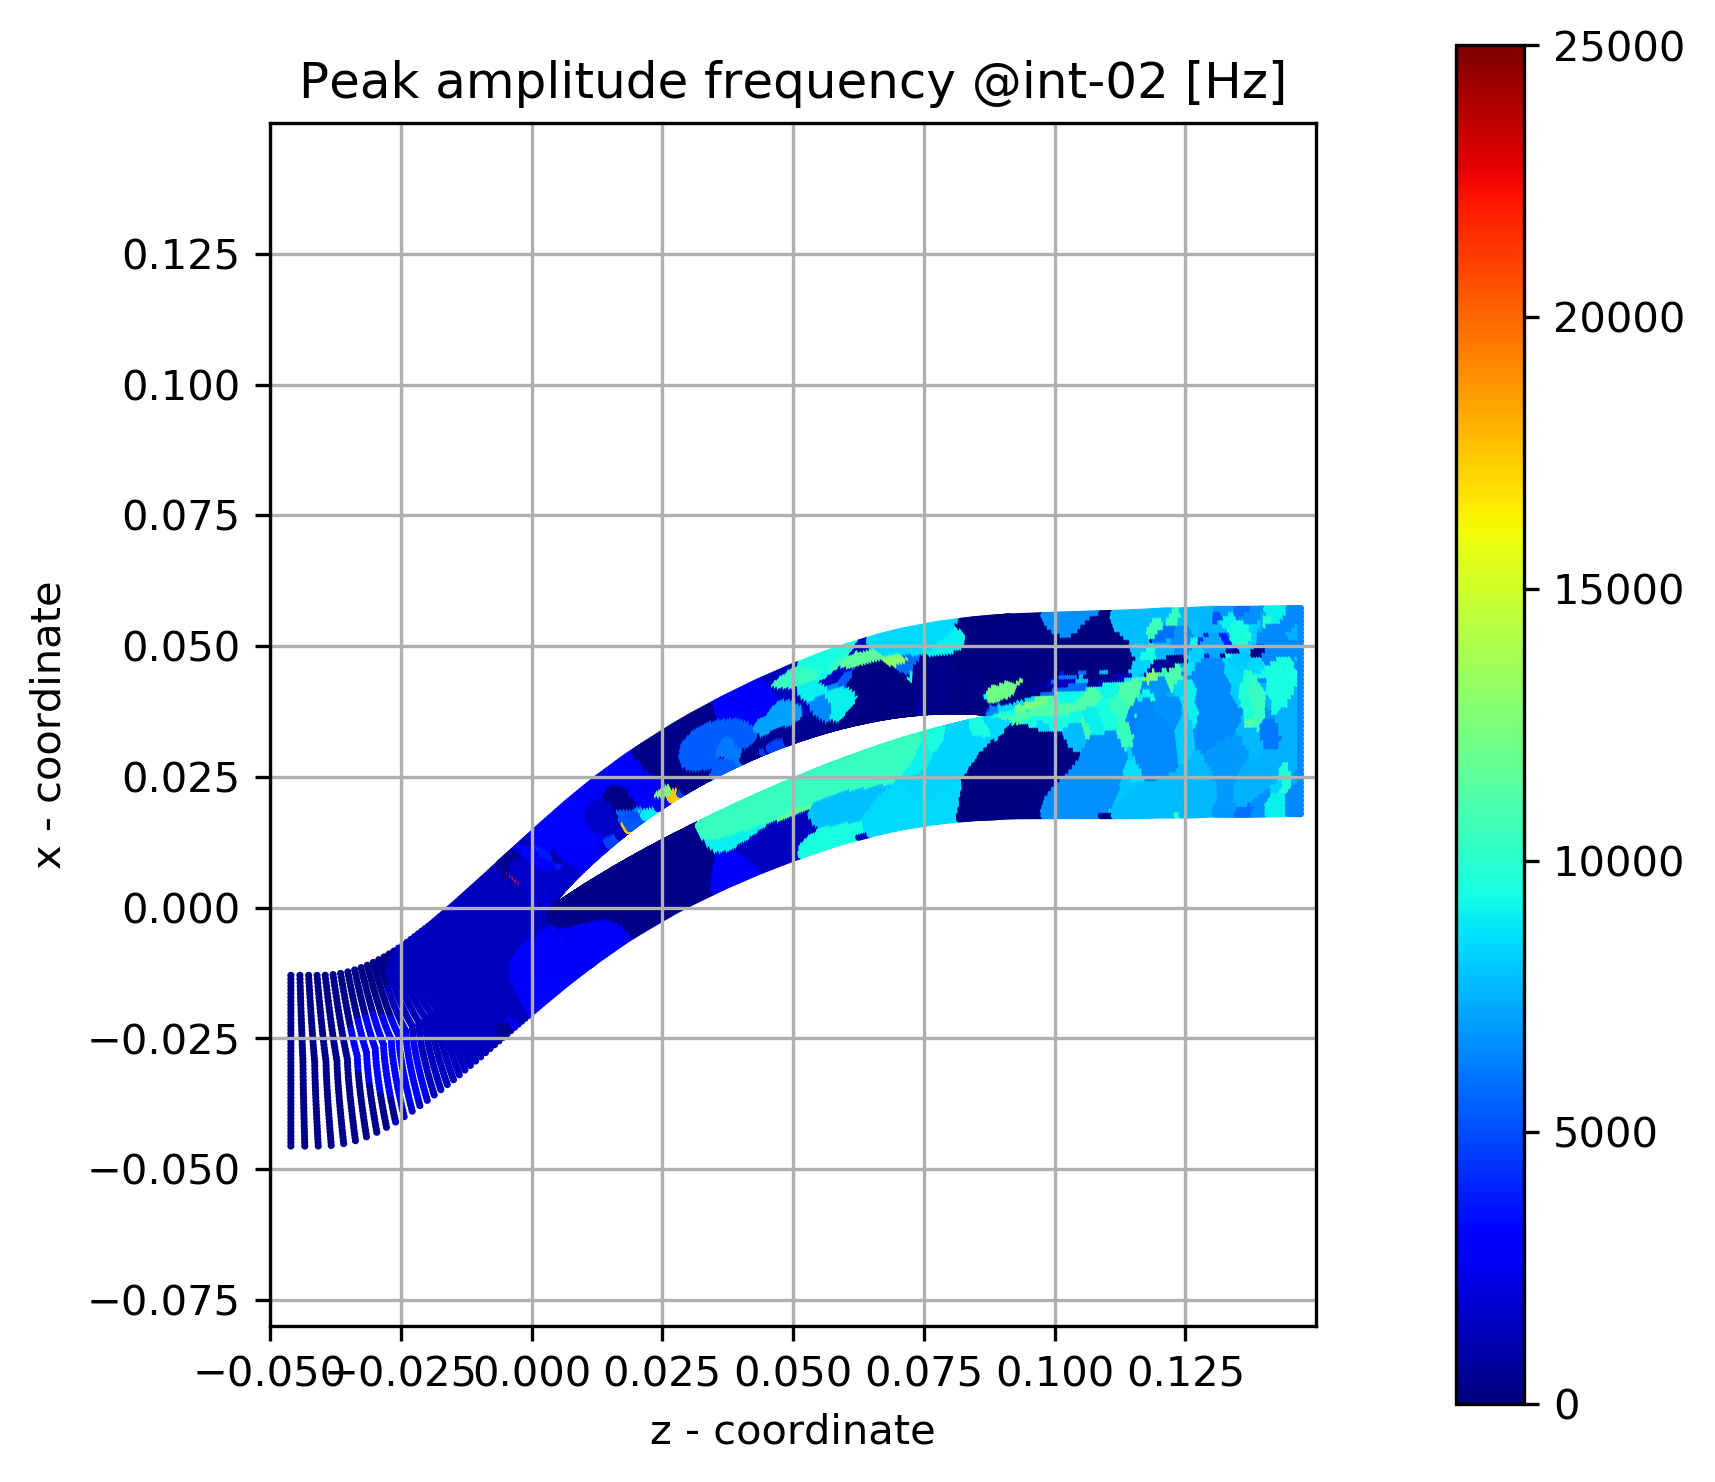
\includegraphics[width=0.75\textwidth]{Figures/int-02-peak-freq.png}
  \caption{Peak amplitude frequency int-02 mark} \label{int-02-peak-freq}
  
  \vspace*{\floatsep}% https://tex.stackexchange.com/q/26521/5764

  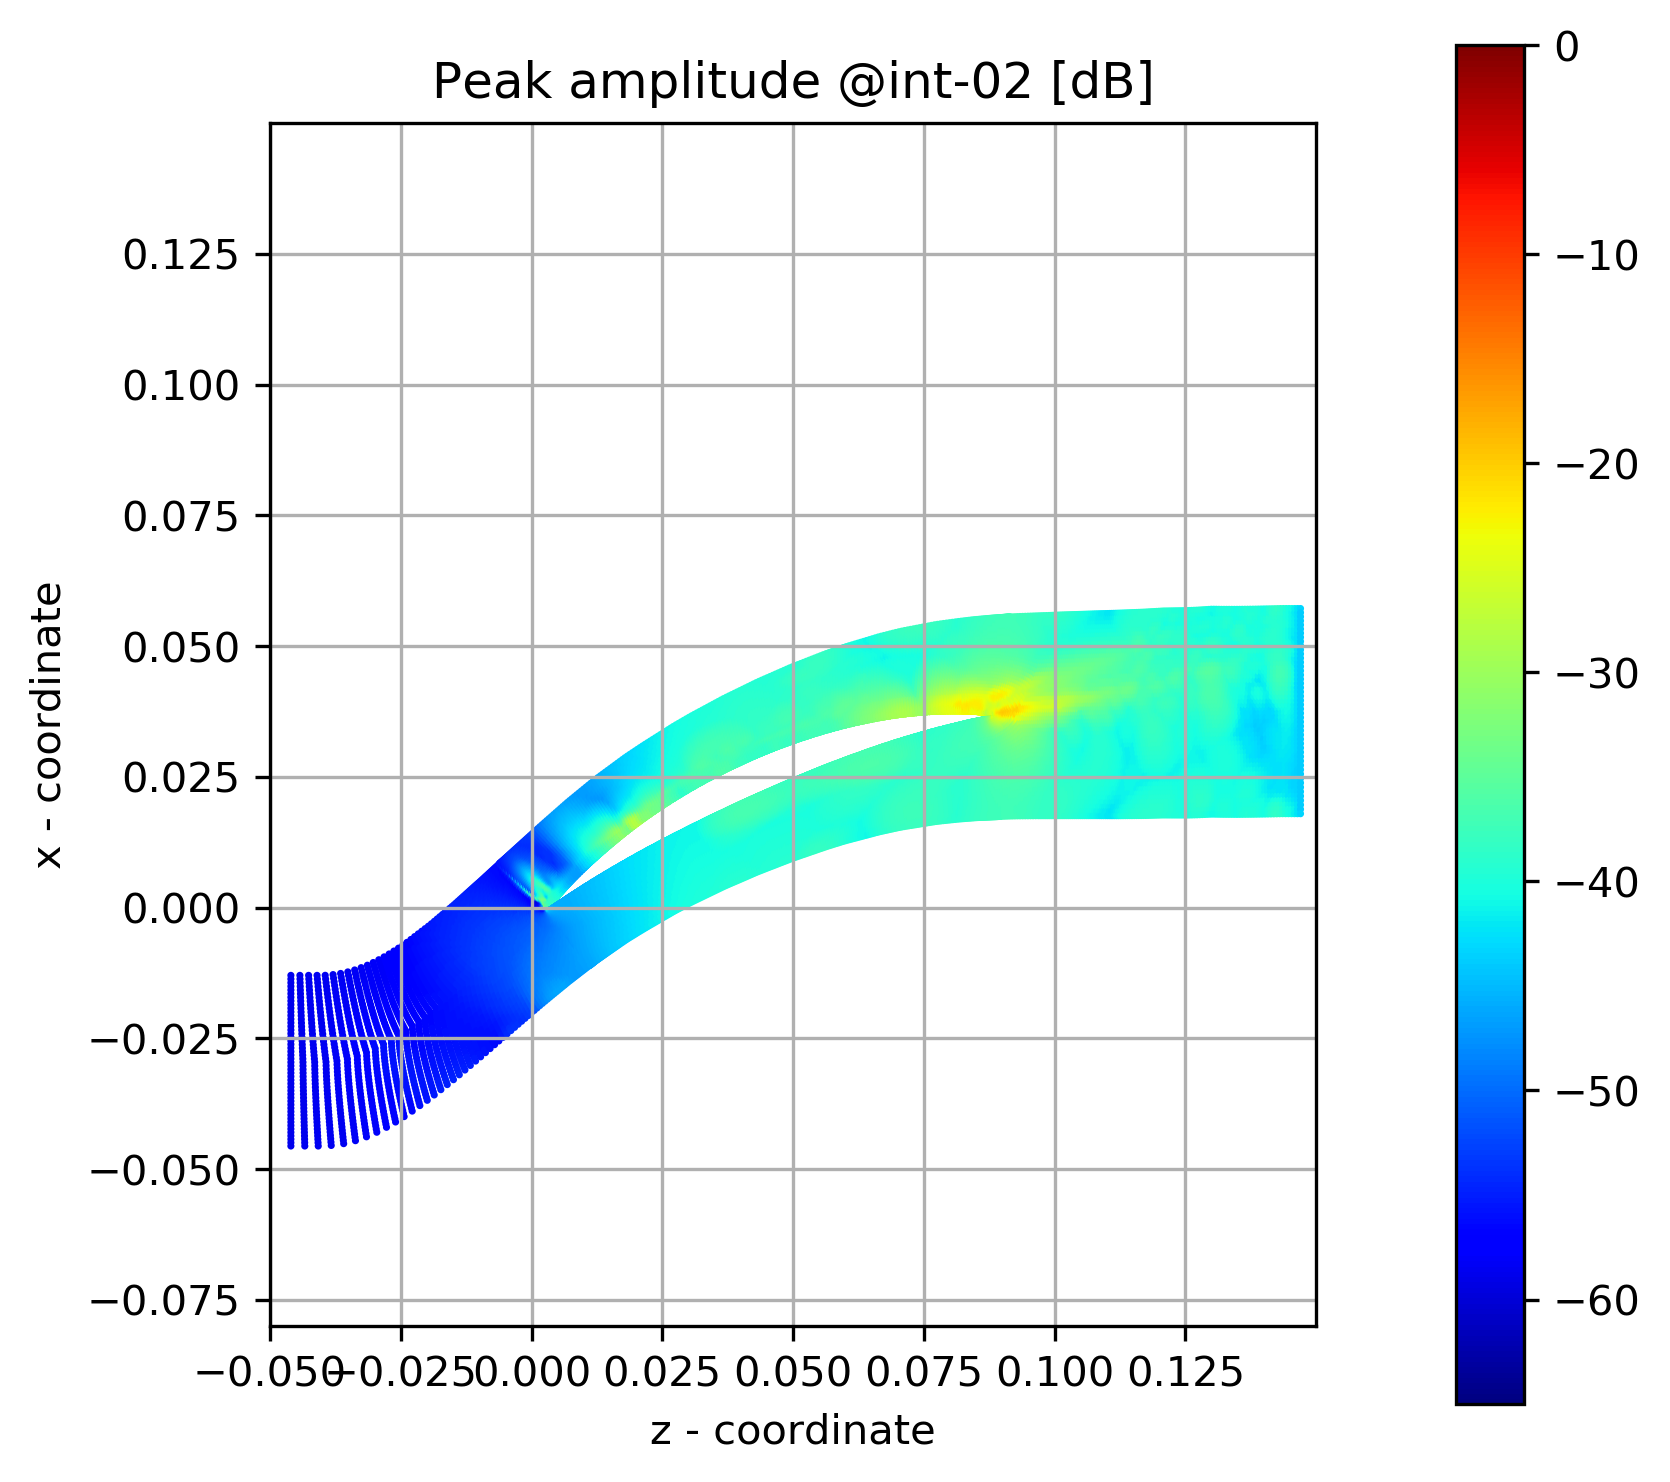
\includegraphics[width=0.75\textwidth]{Figures/int-02-peak-mag.png}
  \caption{Peak magnitude at int-02 mark} \label{int-02-peak-mag}
\end{figure}

%int-03
\begin{figure}[ht]
  \centering
  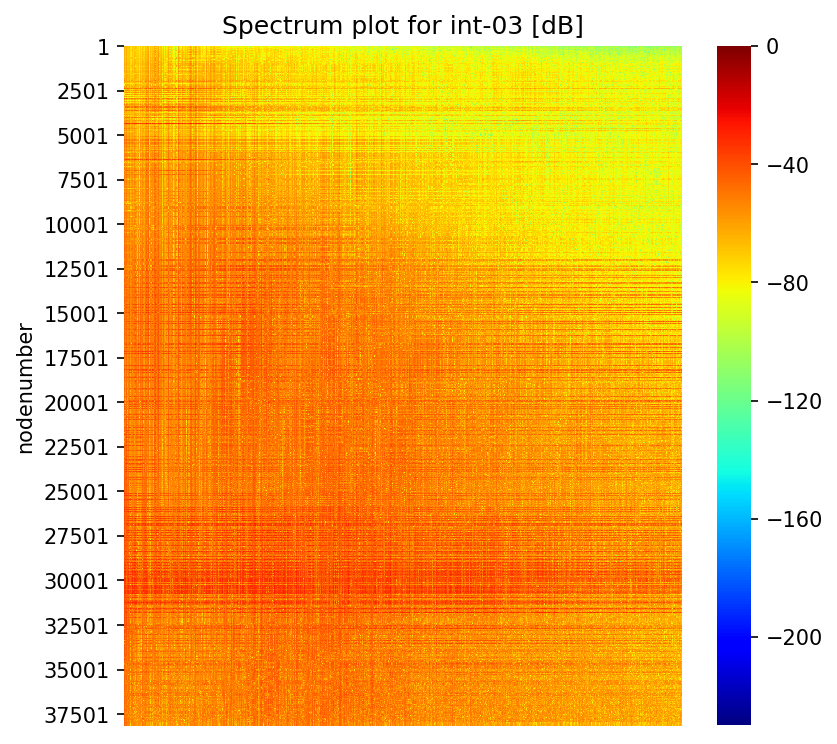
\includegraphics[width=0.75\textwidth]{Figures/int-03_spectrum.png}
  \caption{Spectrum plot at int-03 mark} \label{int-03-spectrum}
  
  \vspace*{\floatsep}% https://tex.stackexchange.com/q/26521/5764

  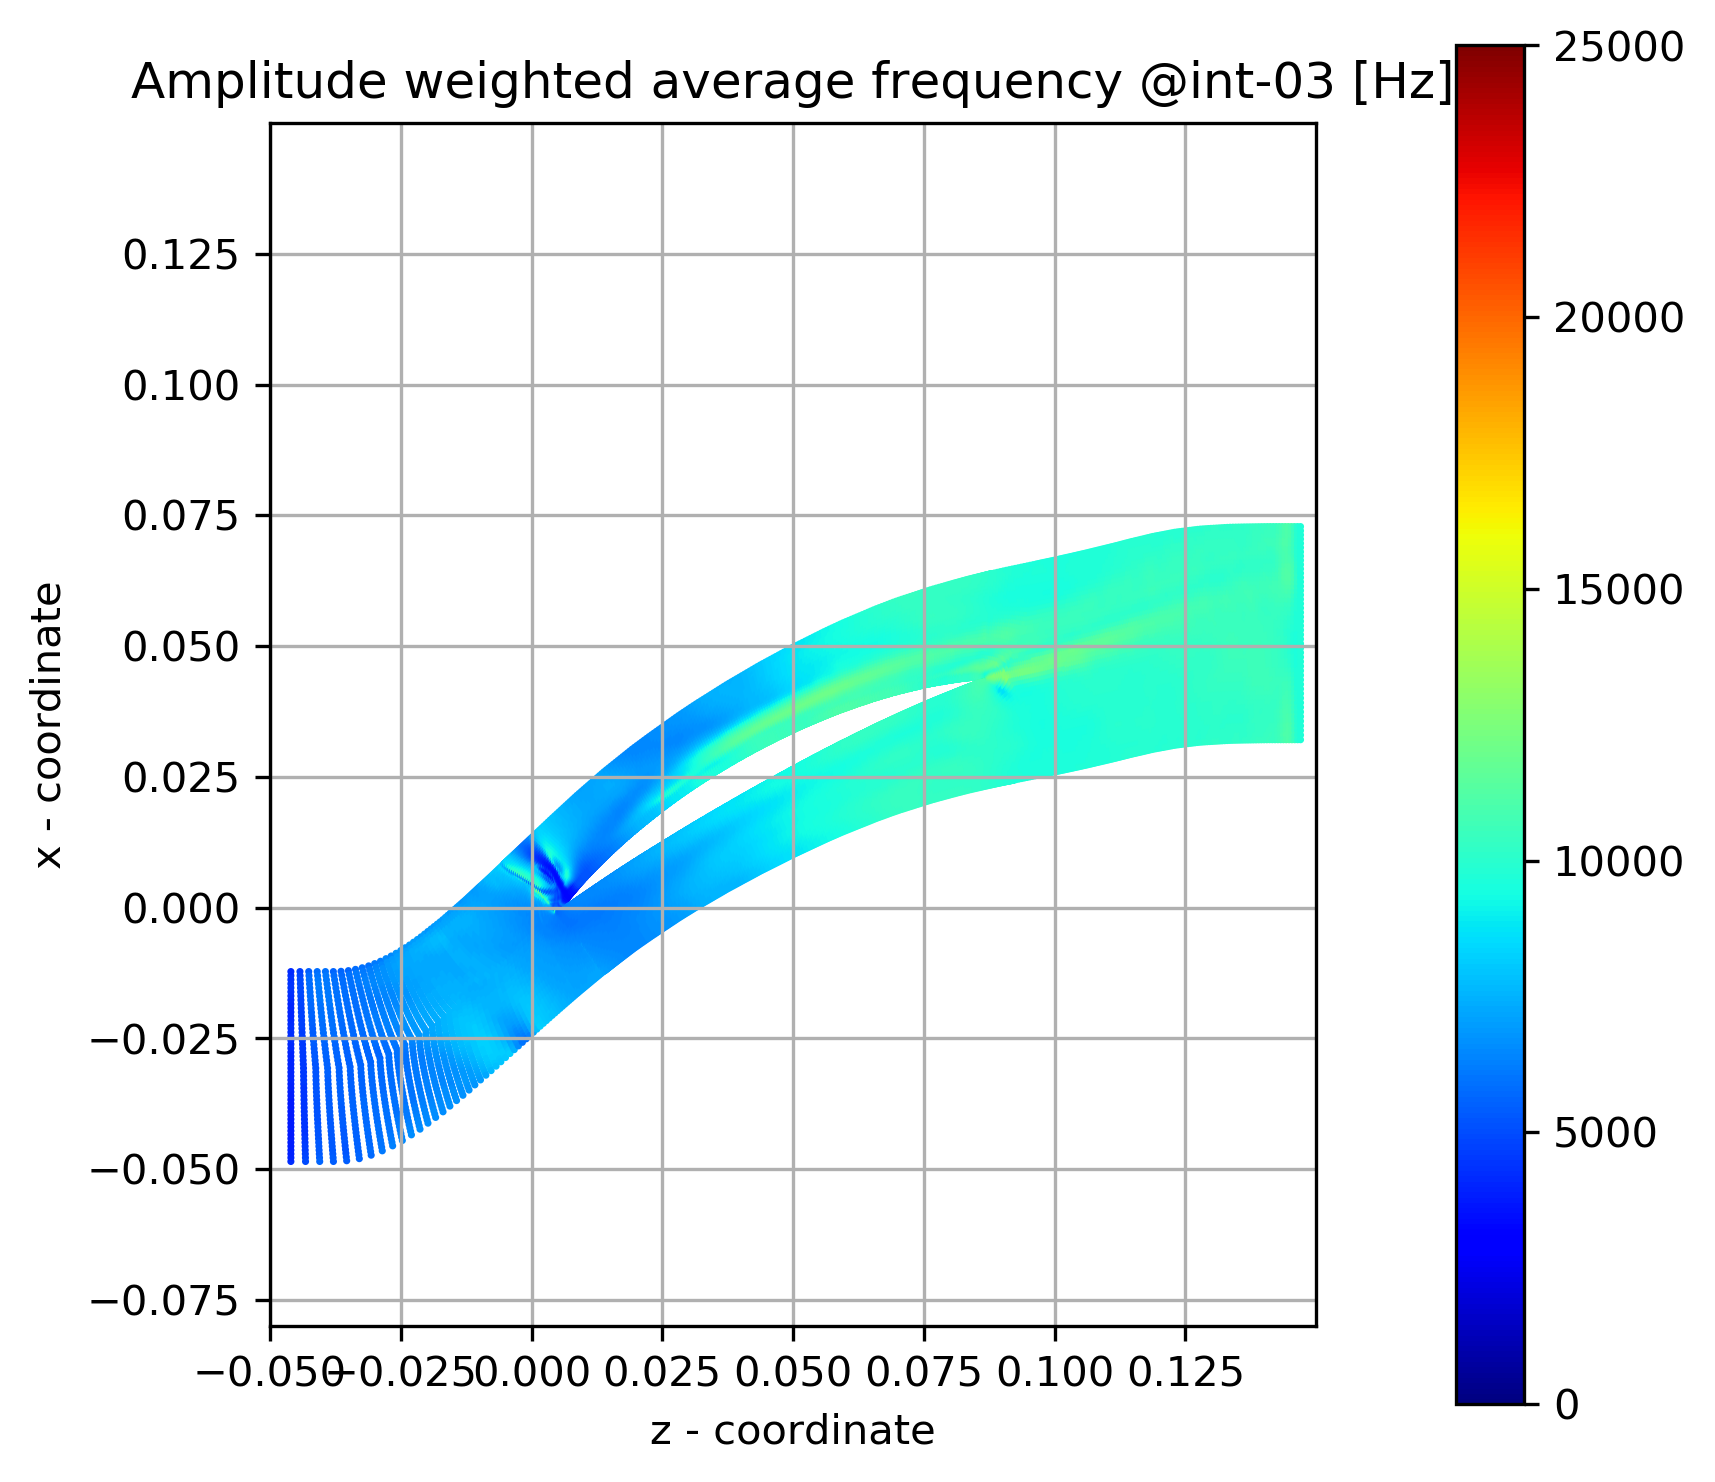
\includegraphics[width=0.75\textwidth]{Figures/int-03-awaf.png}
  \caption{Amplitude weighted average frequency at int-03 mark} \label{int-03-awaf}
\end{figure}
%int-03
\begin{figure}[ht]
  \centering
  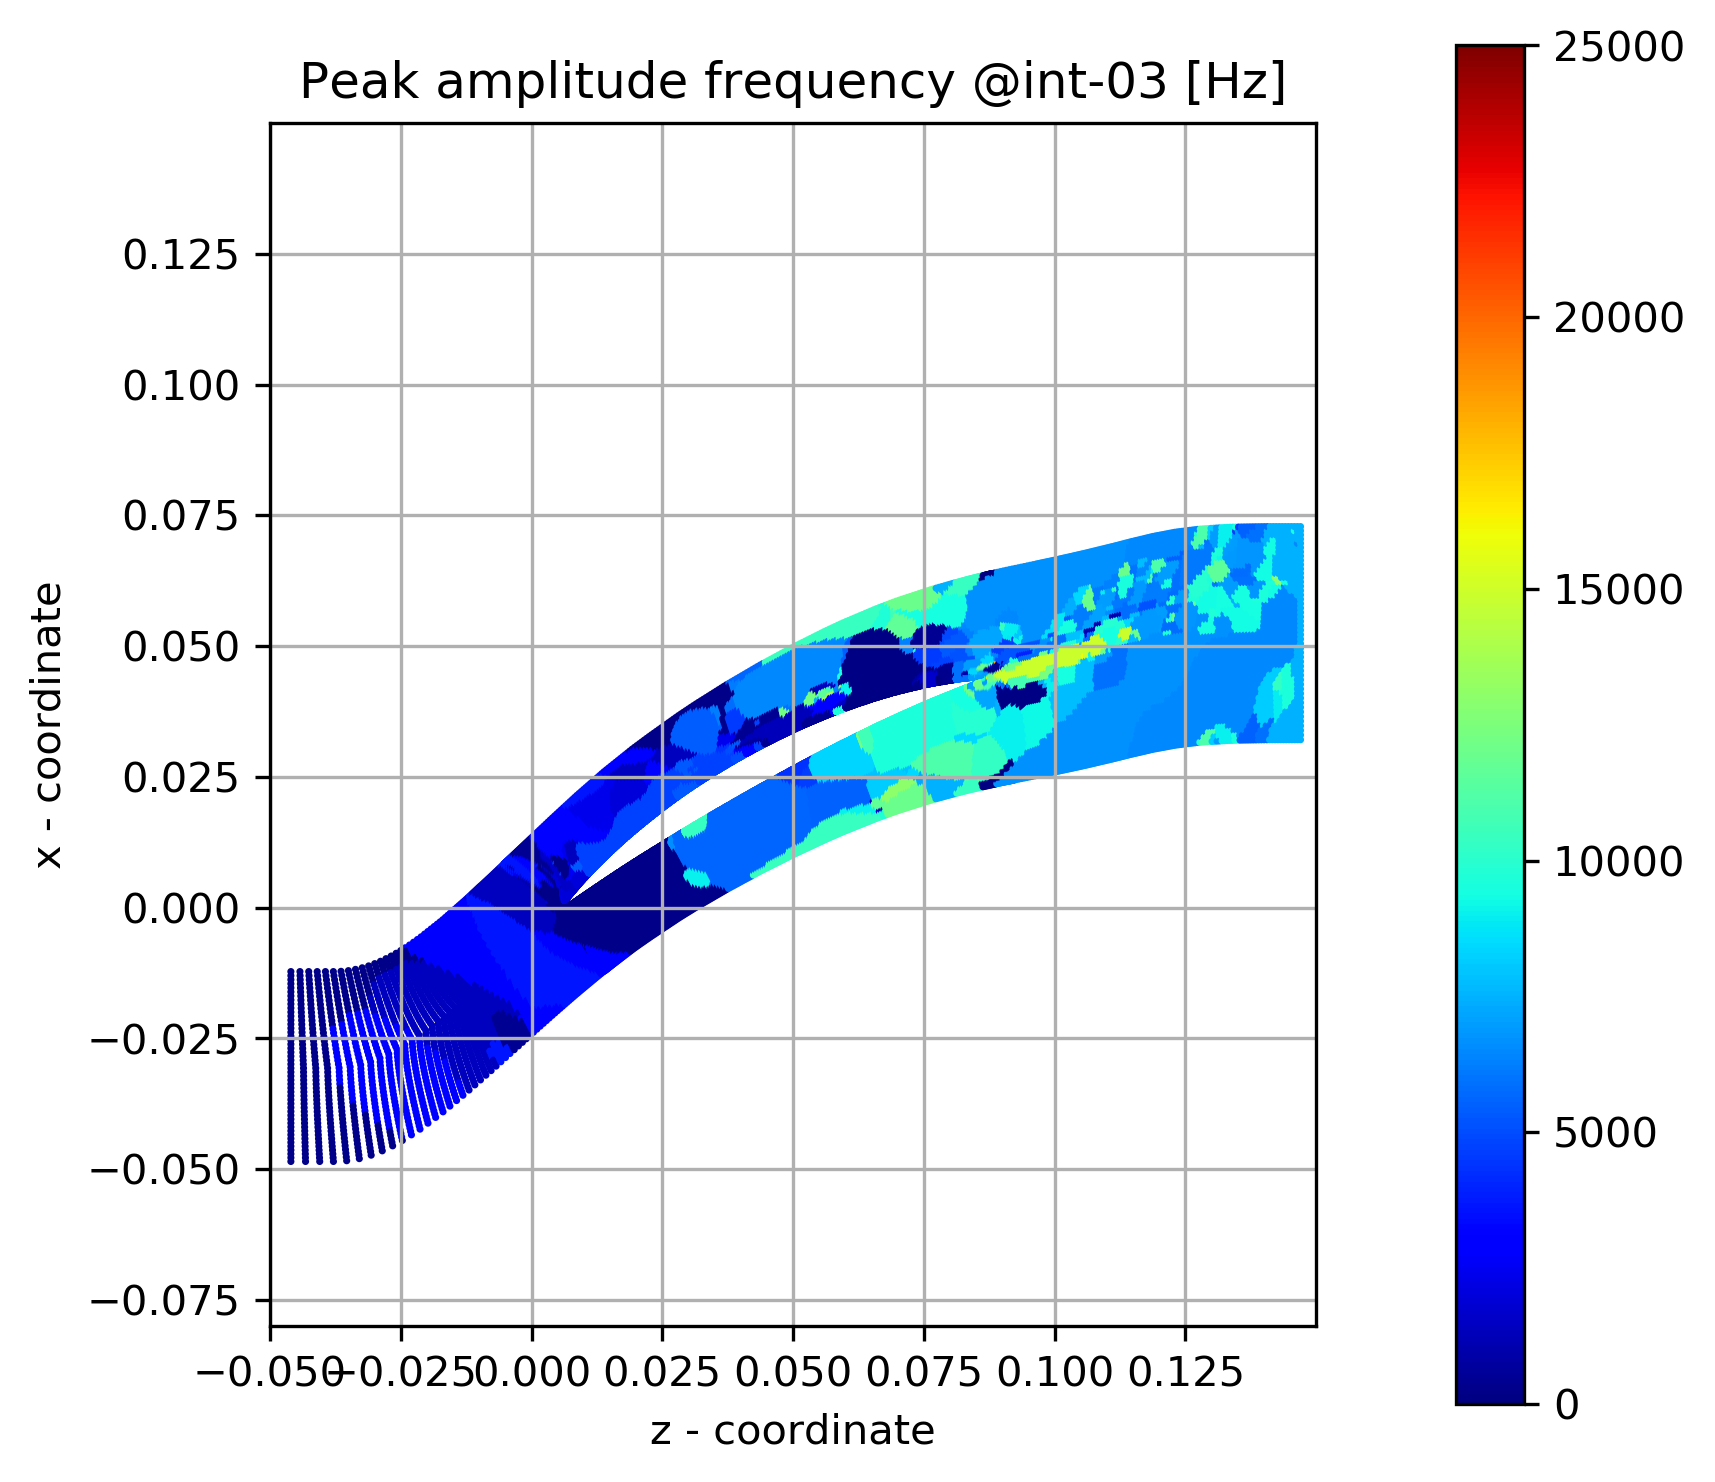
\includegraphics[width=0.75\textwidth]{Figures/int-03-peak-freq.png}
  \caption{Peak amplitude frequency int-03 mark} \label{int-03-peak-freq}
  
  \vspace*{\floatsep}% https://tex.stackexchange.com/q/26521/5764

  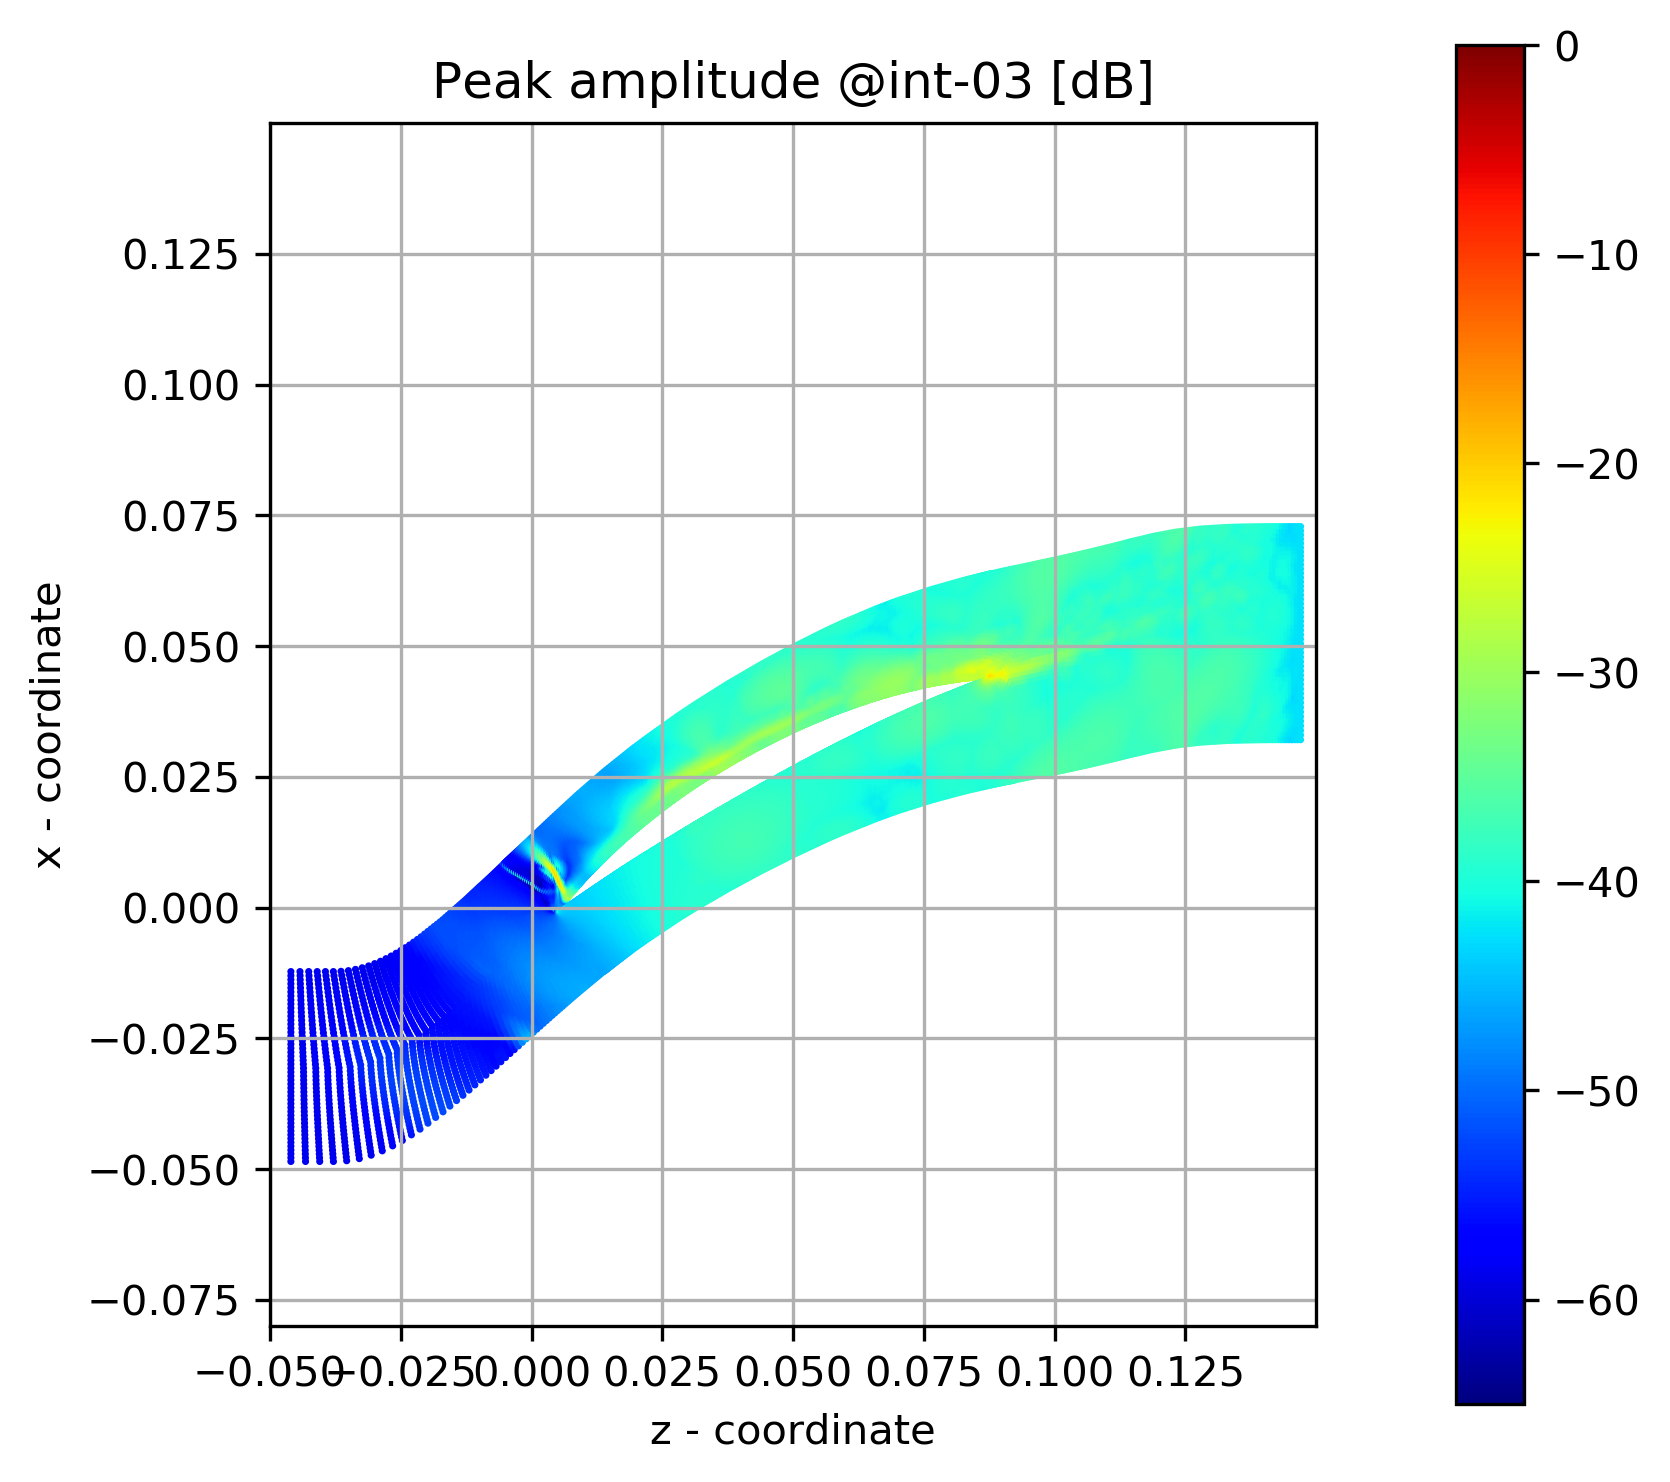
\includegraphics[width=0.75\textwidth]{Figures/int-03-peak-mag.png}
  \caption{Peak magnitude at int-03 mark} \label{int-03-peak-mag}
\end{figure}

%int-04
\begin{figure}[ht]
  \centering
  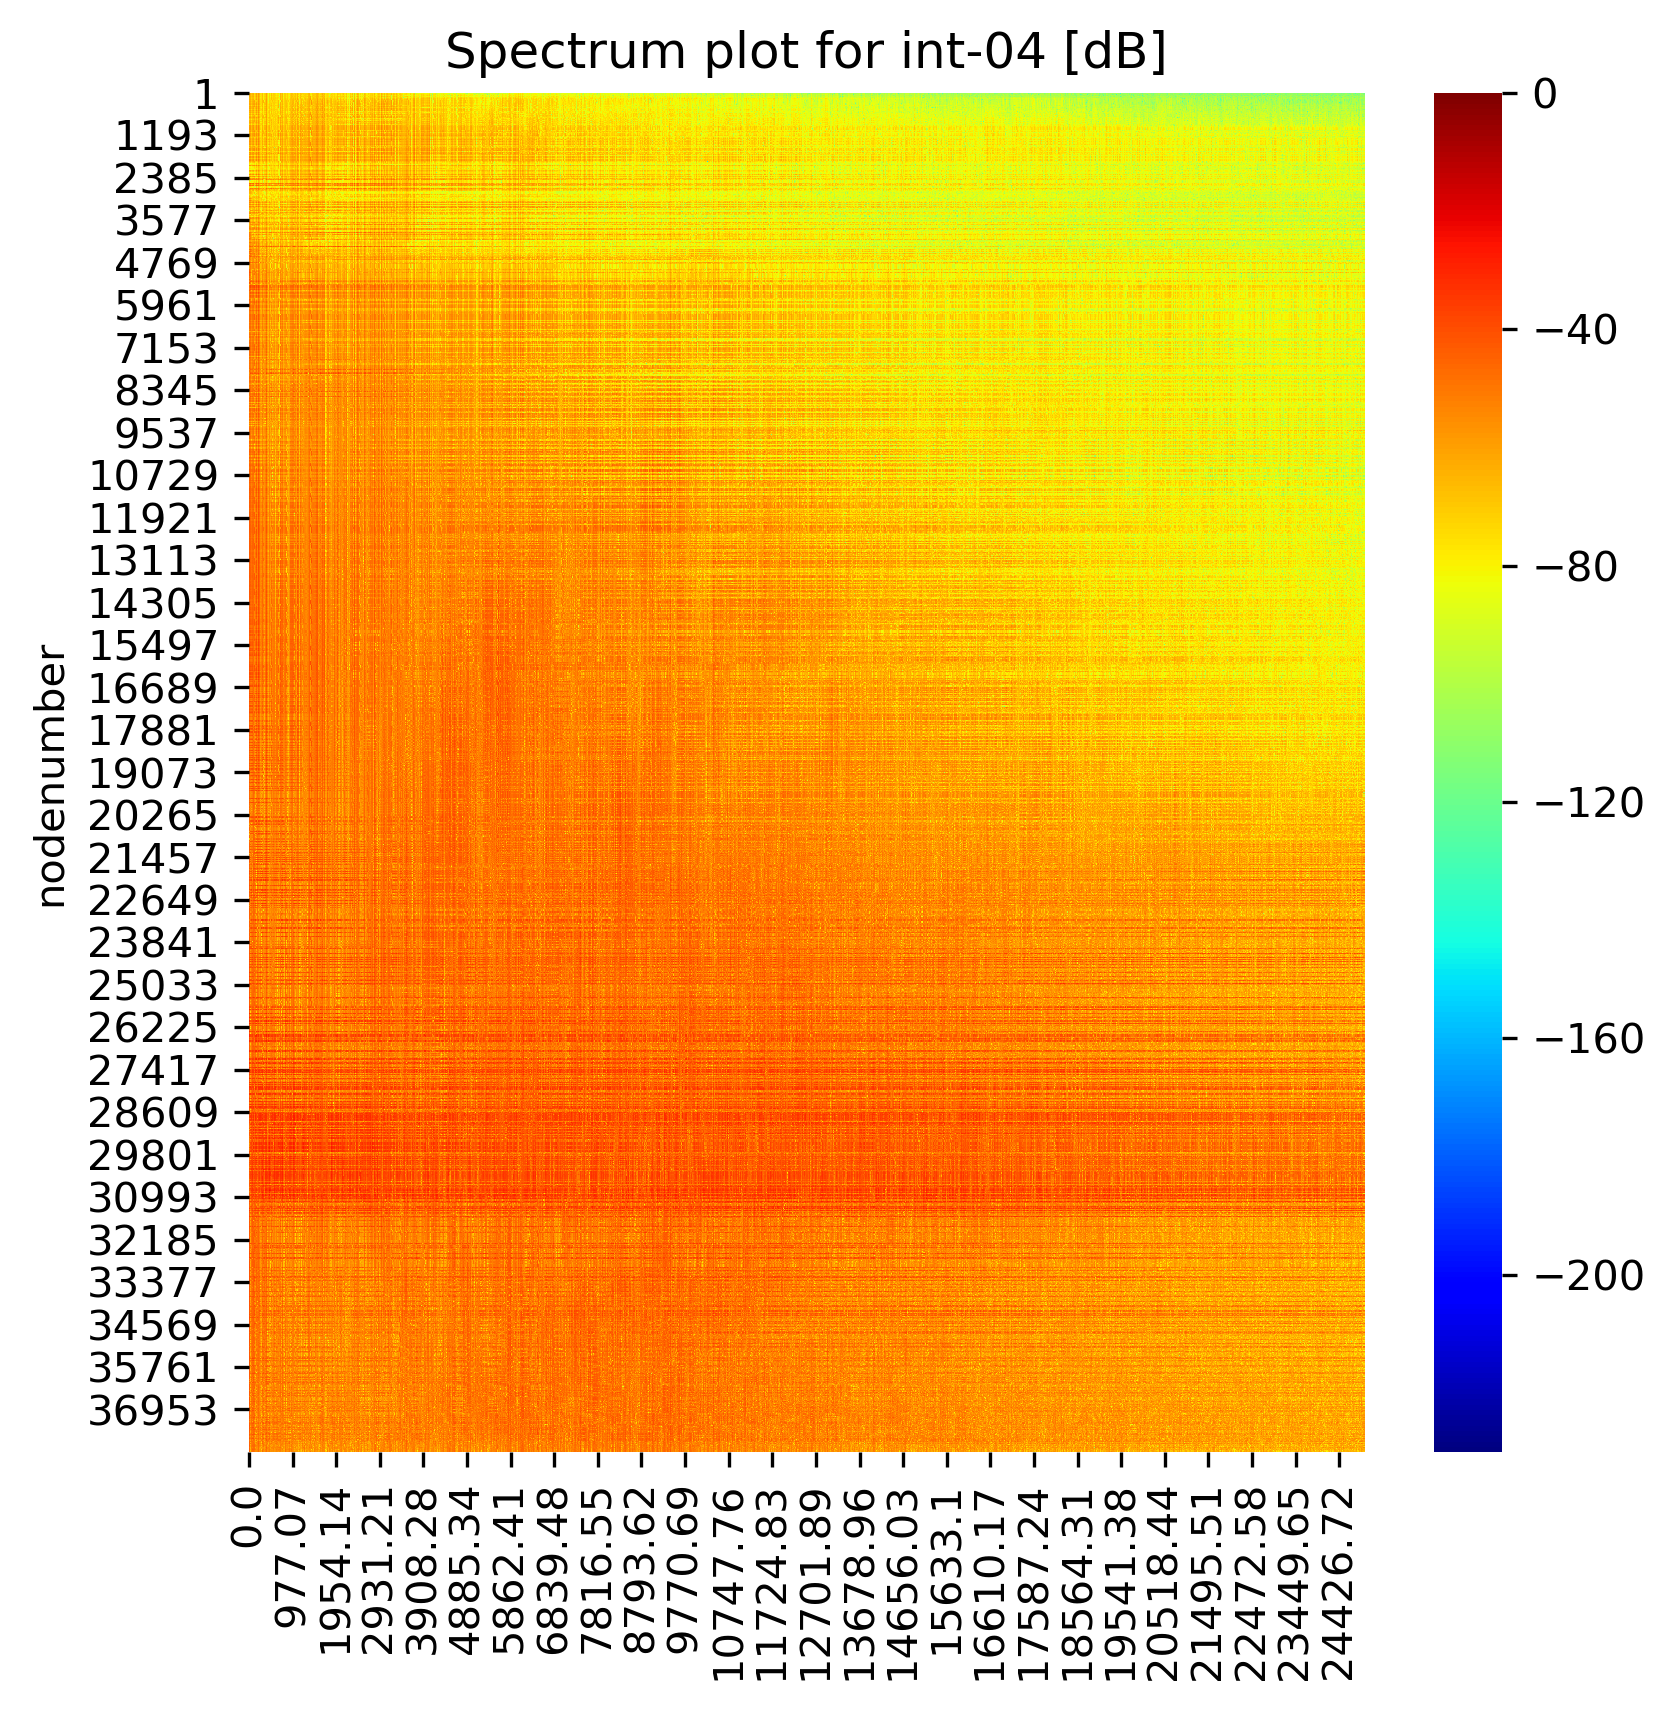
\includegraphics[width=0.75\textwidth]{Figures/int-04_spectrum.png}
  \caption{Spectrum plot at int-04 mark} \label{int-04-spectrum}
  
  \vspace*{\floatsep}% https://tex.stackexchange.com/q/26521/5764

  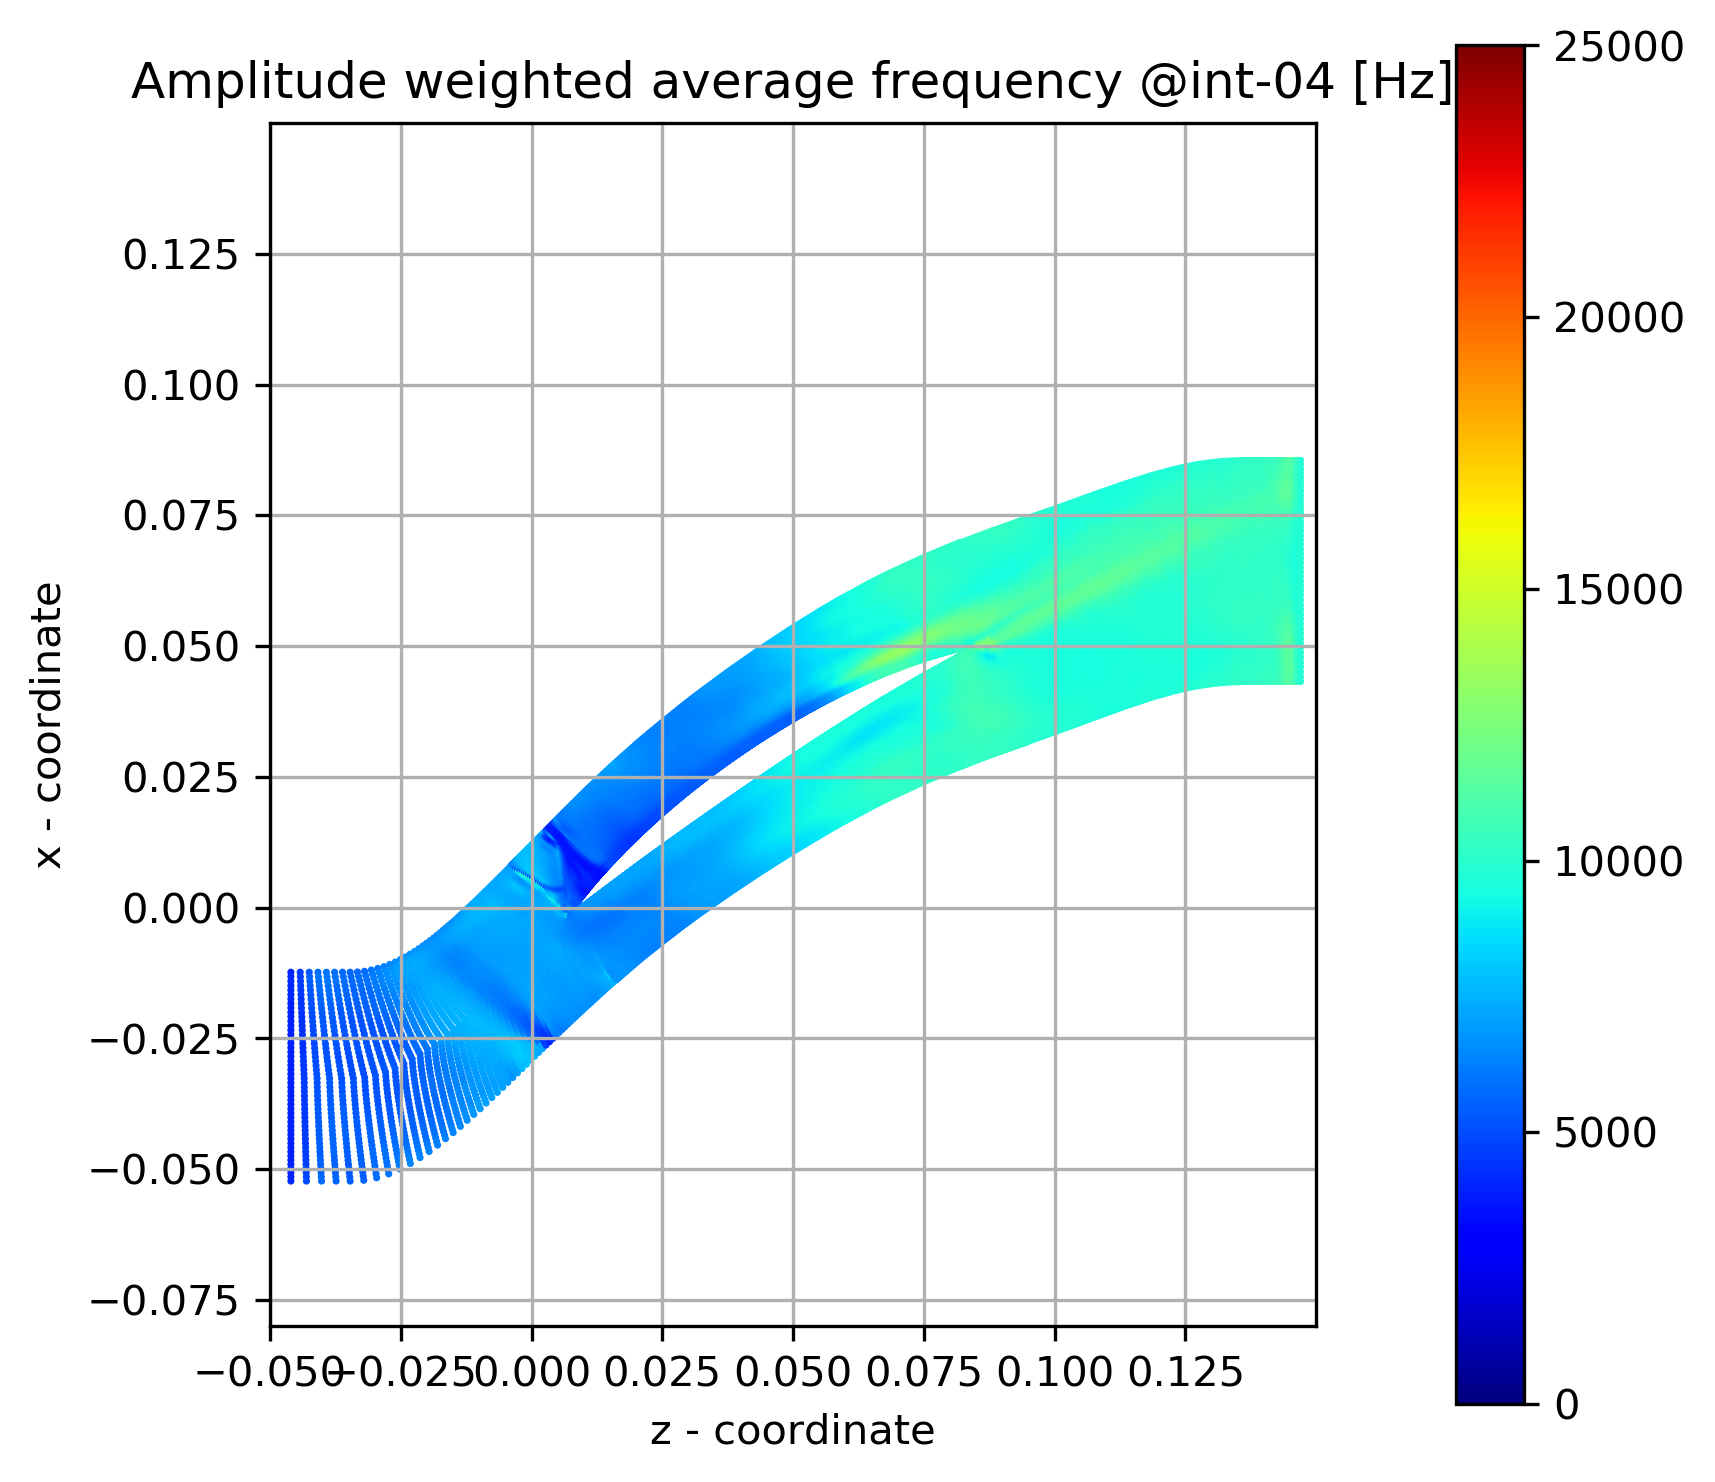
\includegraphics[width=0.75\textwidth]{Figures/int-04-awaf.png}
  \caption{Amplitude weighted average frequency at int-04 mark} \label{int-04-awaf}
\end{figure}
%int-04
\begin{figure}[ht]
  \centering
  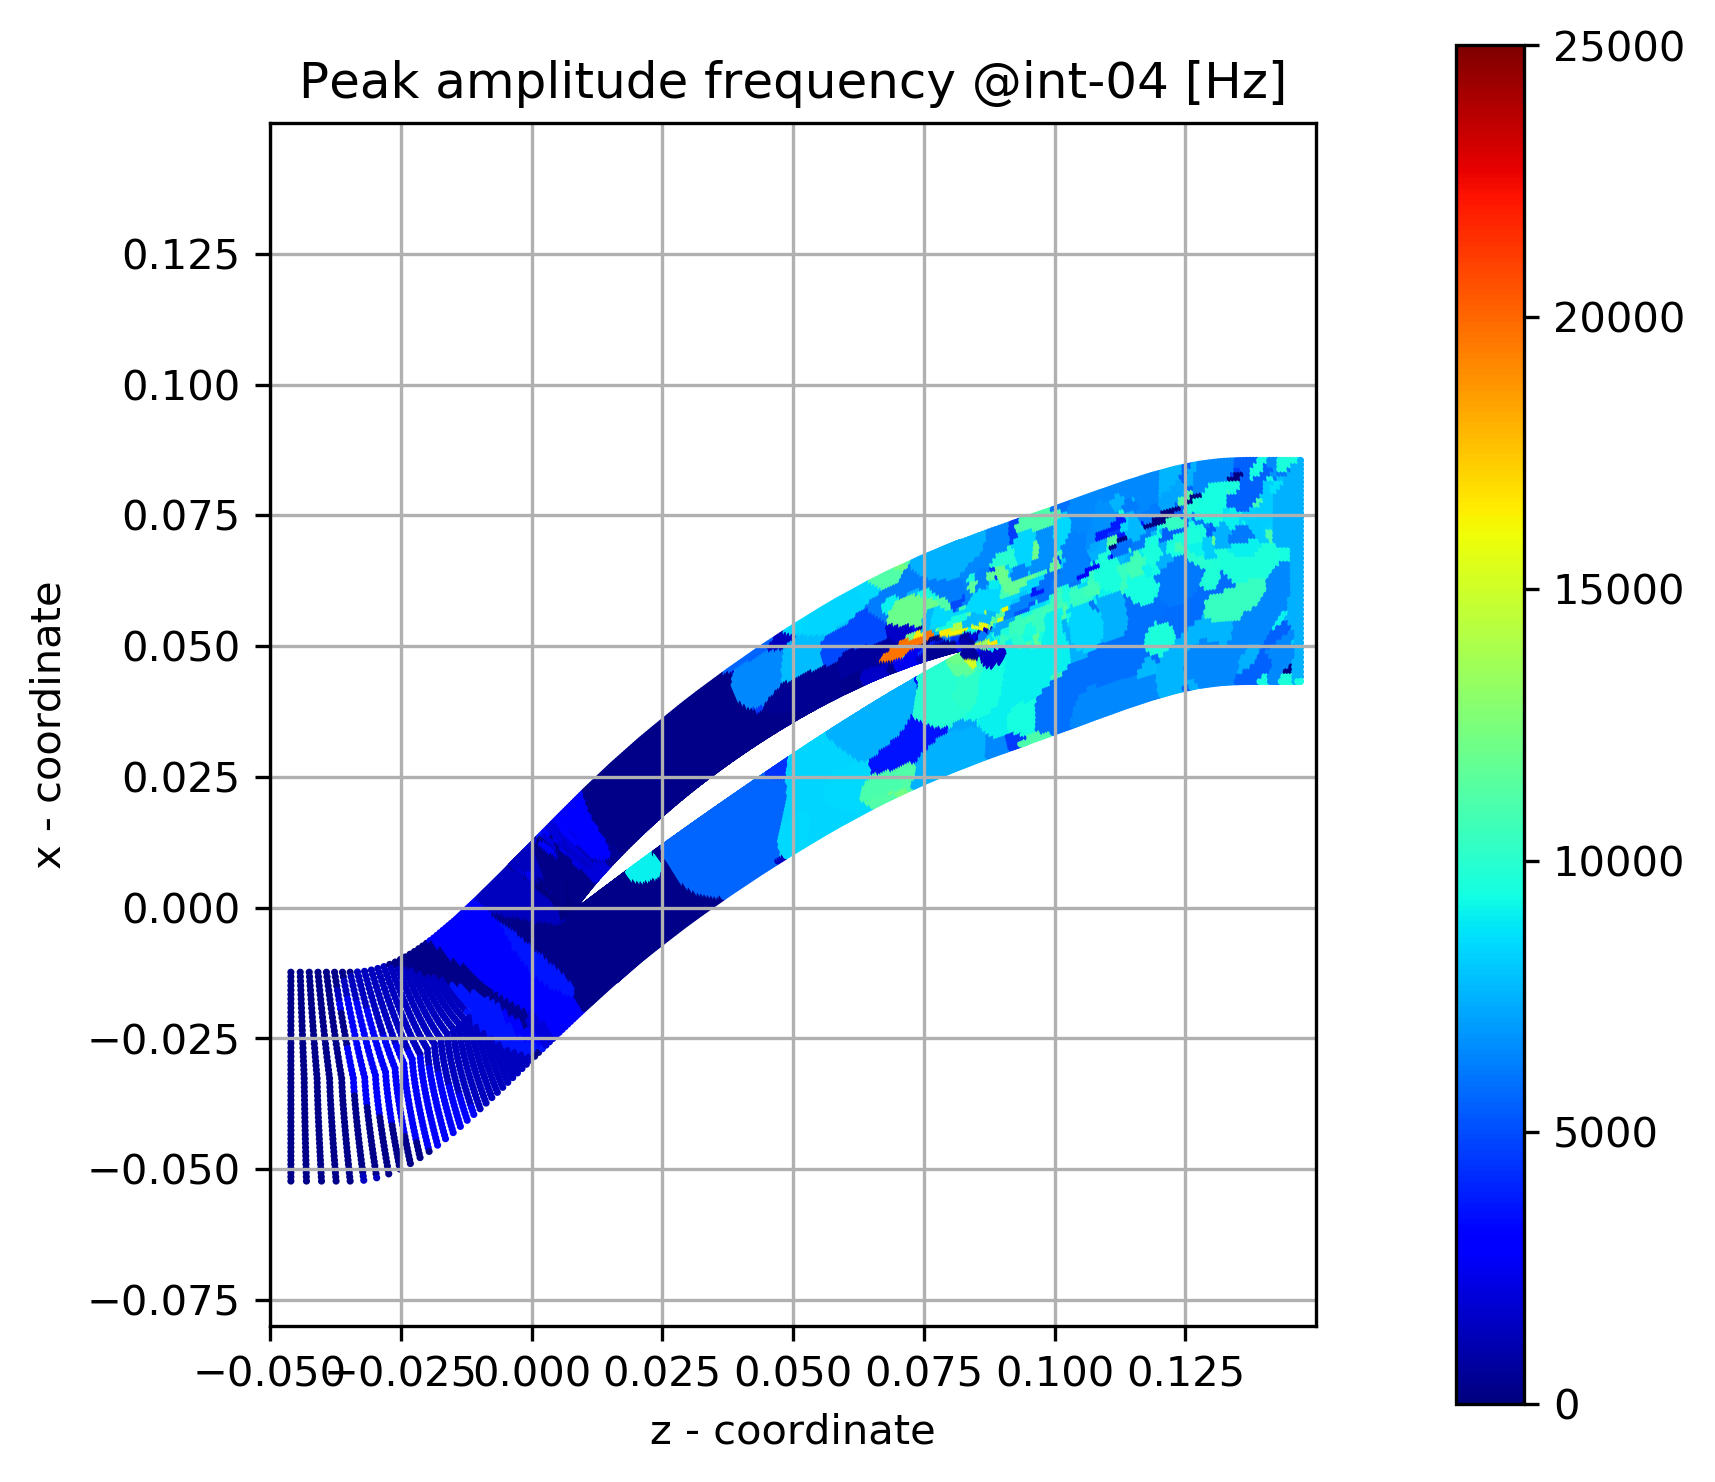
\includegraphics[width=0.75\textwidth]{Figures/int-04-peak-freq.png}
  \caption{Peak amplitude frequency int-04 mark} \label{int-04-peak-freq}
  
  \vspace*{\floatsep}% https://tex.stackexchange.com/q/26521/5764

  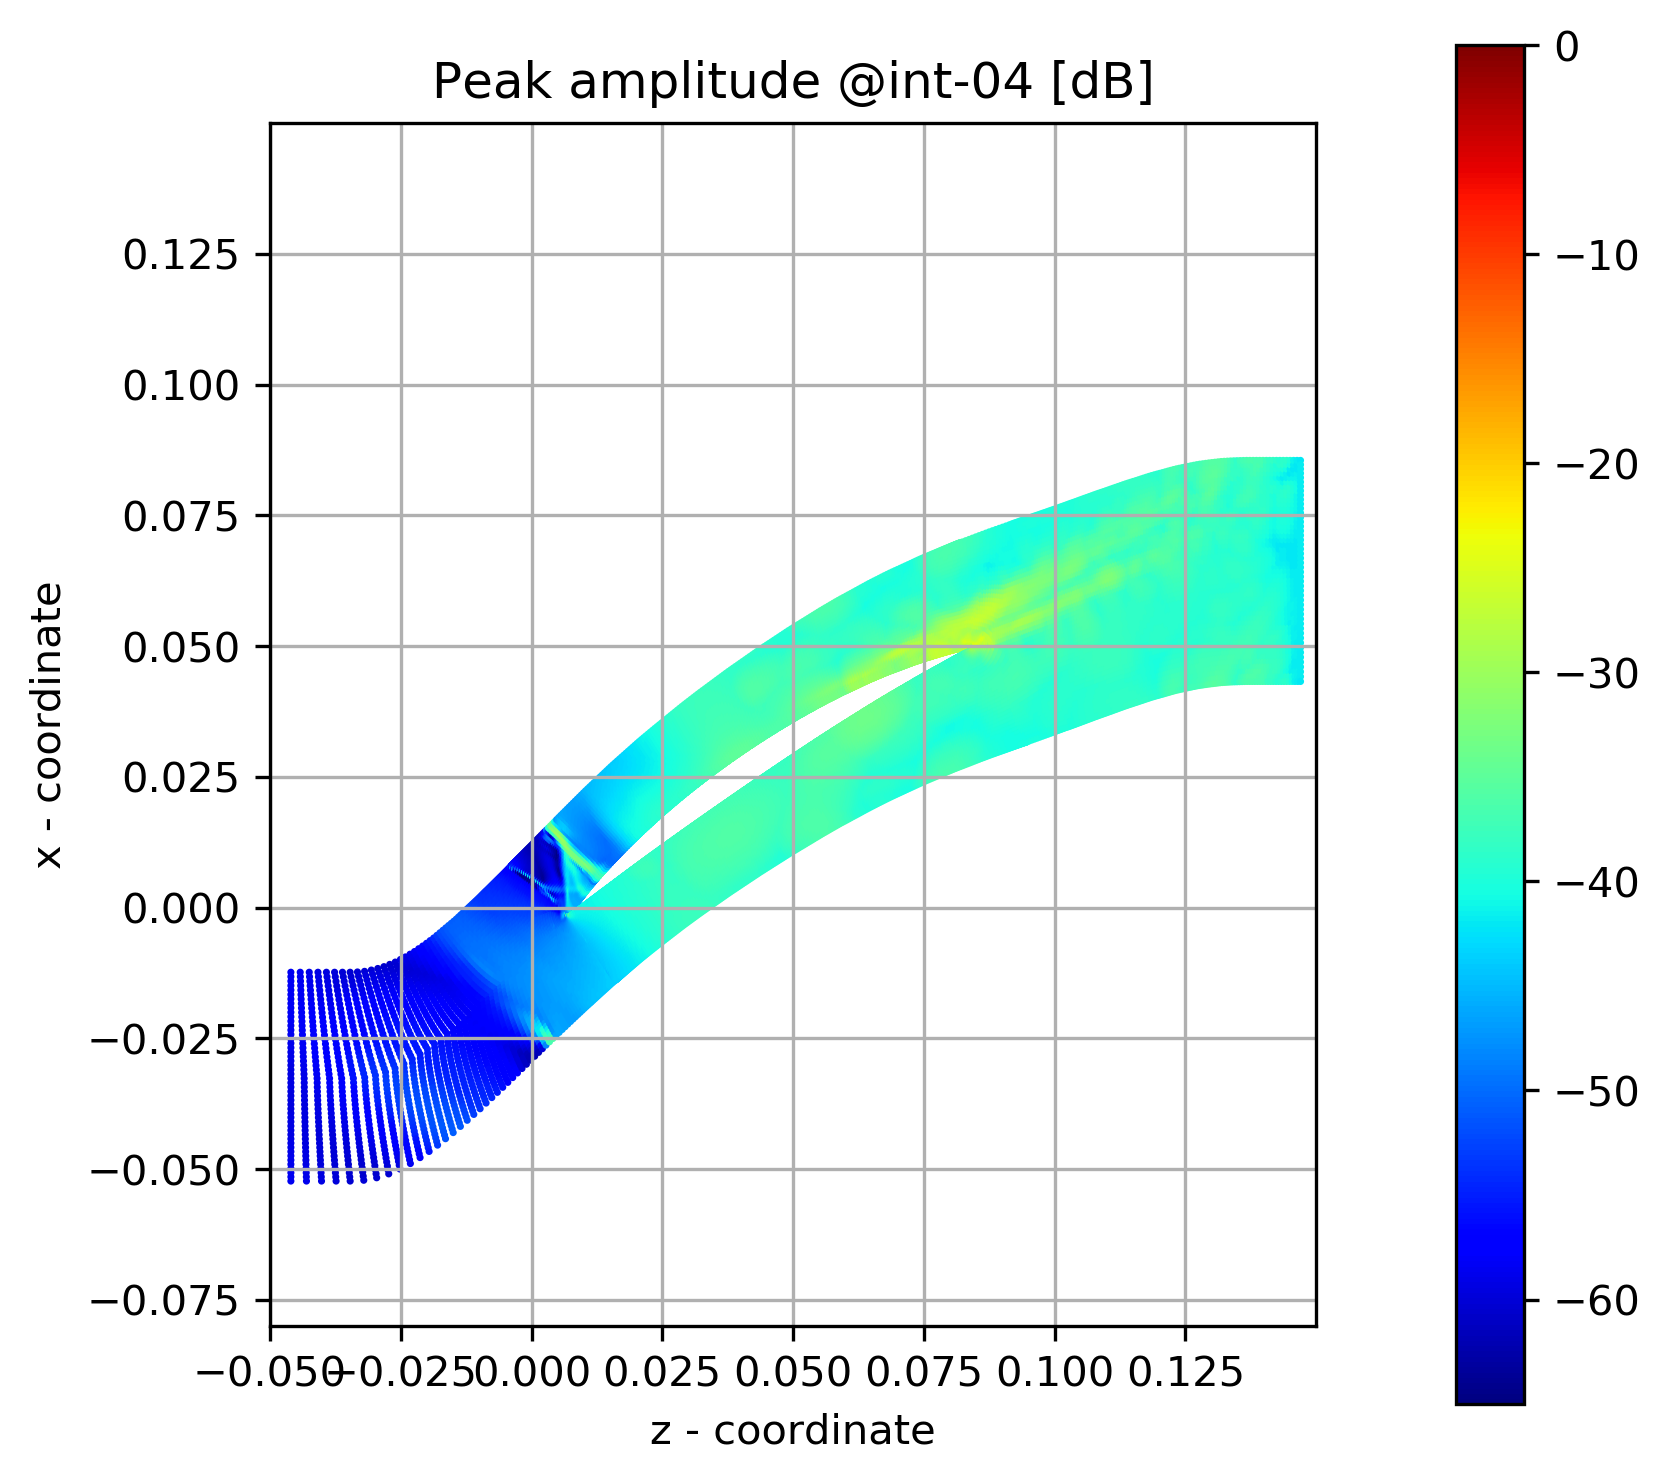
\includegraphics[width=0.75\textwidth]{Figures/int-04-peak-mag.png}
  \caption{Peak magnitude at int-04 mark} \label{int-04-peak-mag}
\end{figure}

%int-05
\begin{figure}[ht]
  \centering
  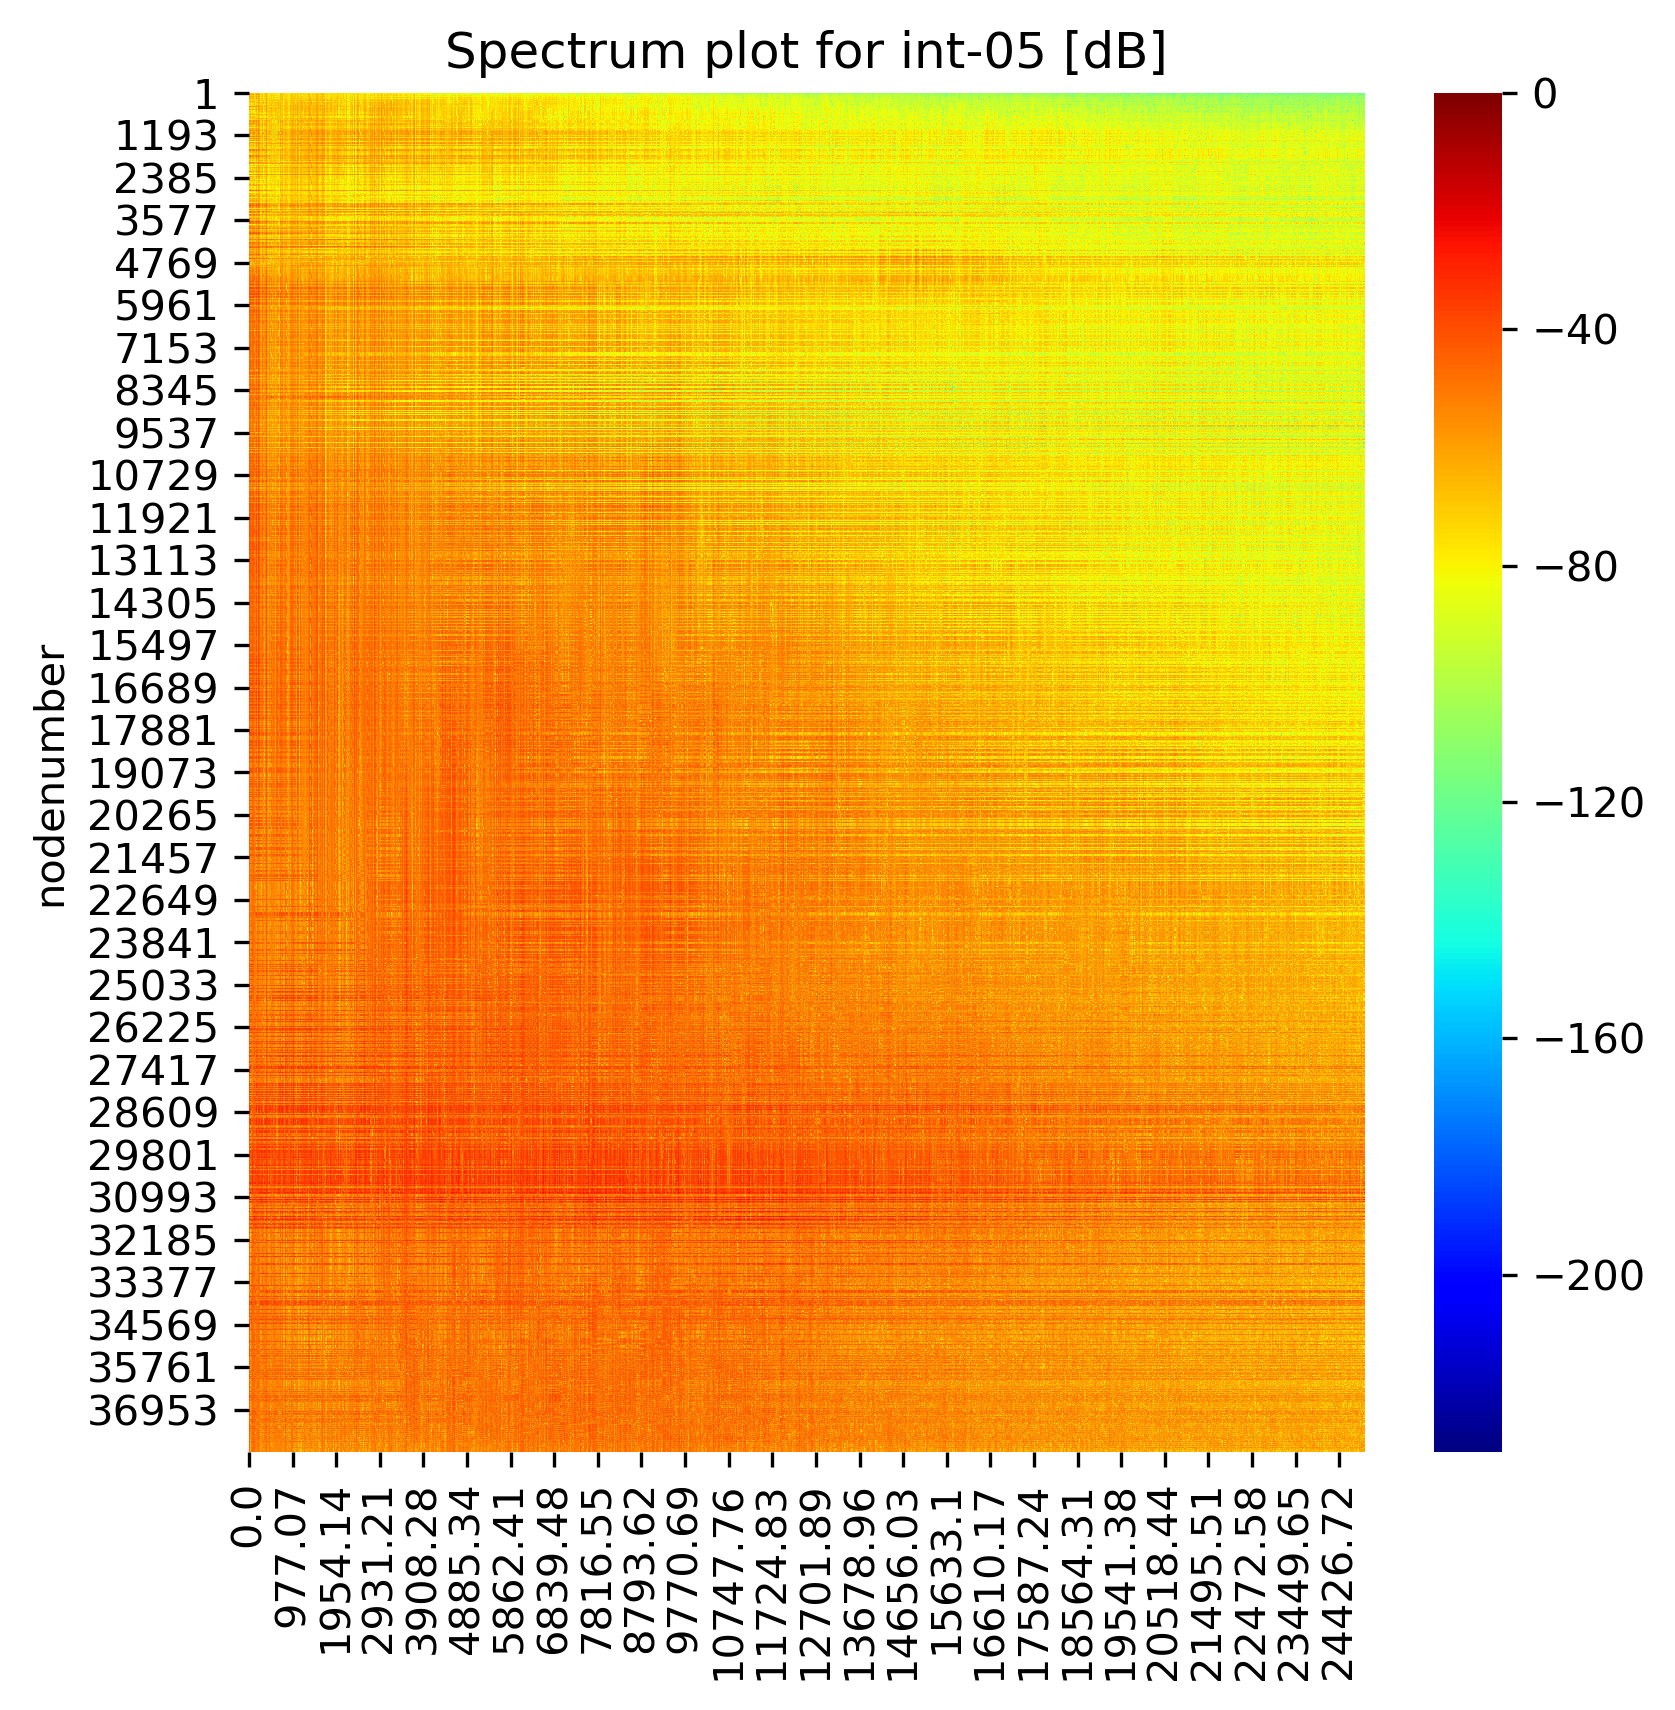
\includegraphics[width=0.75\textwidth]{Figures/int-05_spectrum.png}
  \caption{Spectrum plot at int-05 mark} \label{int-05-spectrum}
  
  \vspace*{\floatsep}% https://tex.stackexchange.com/q/26521/5764

  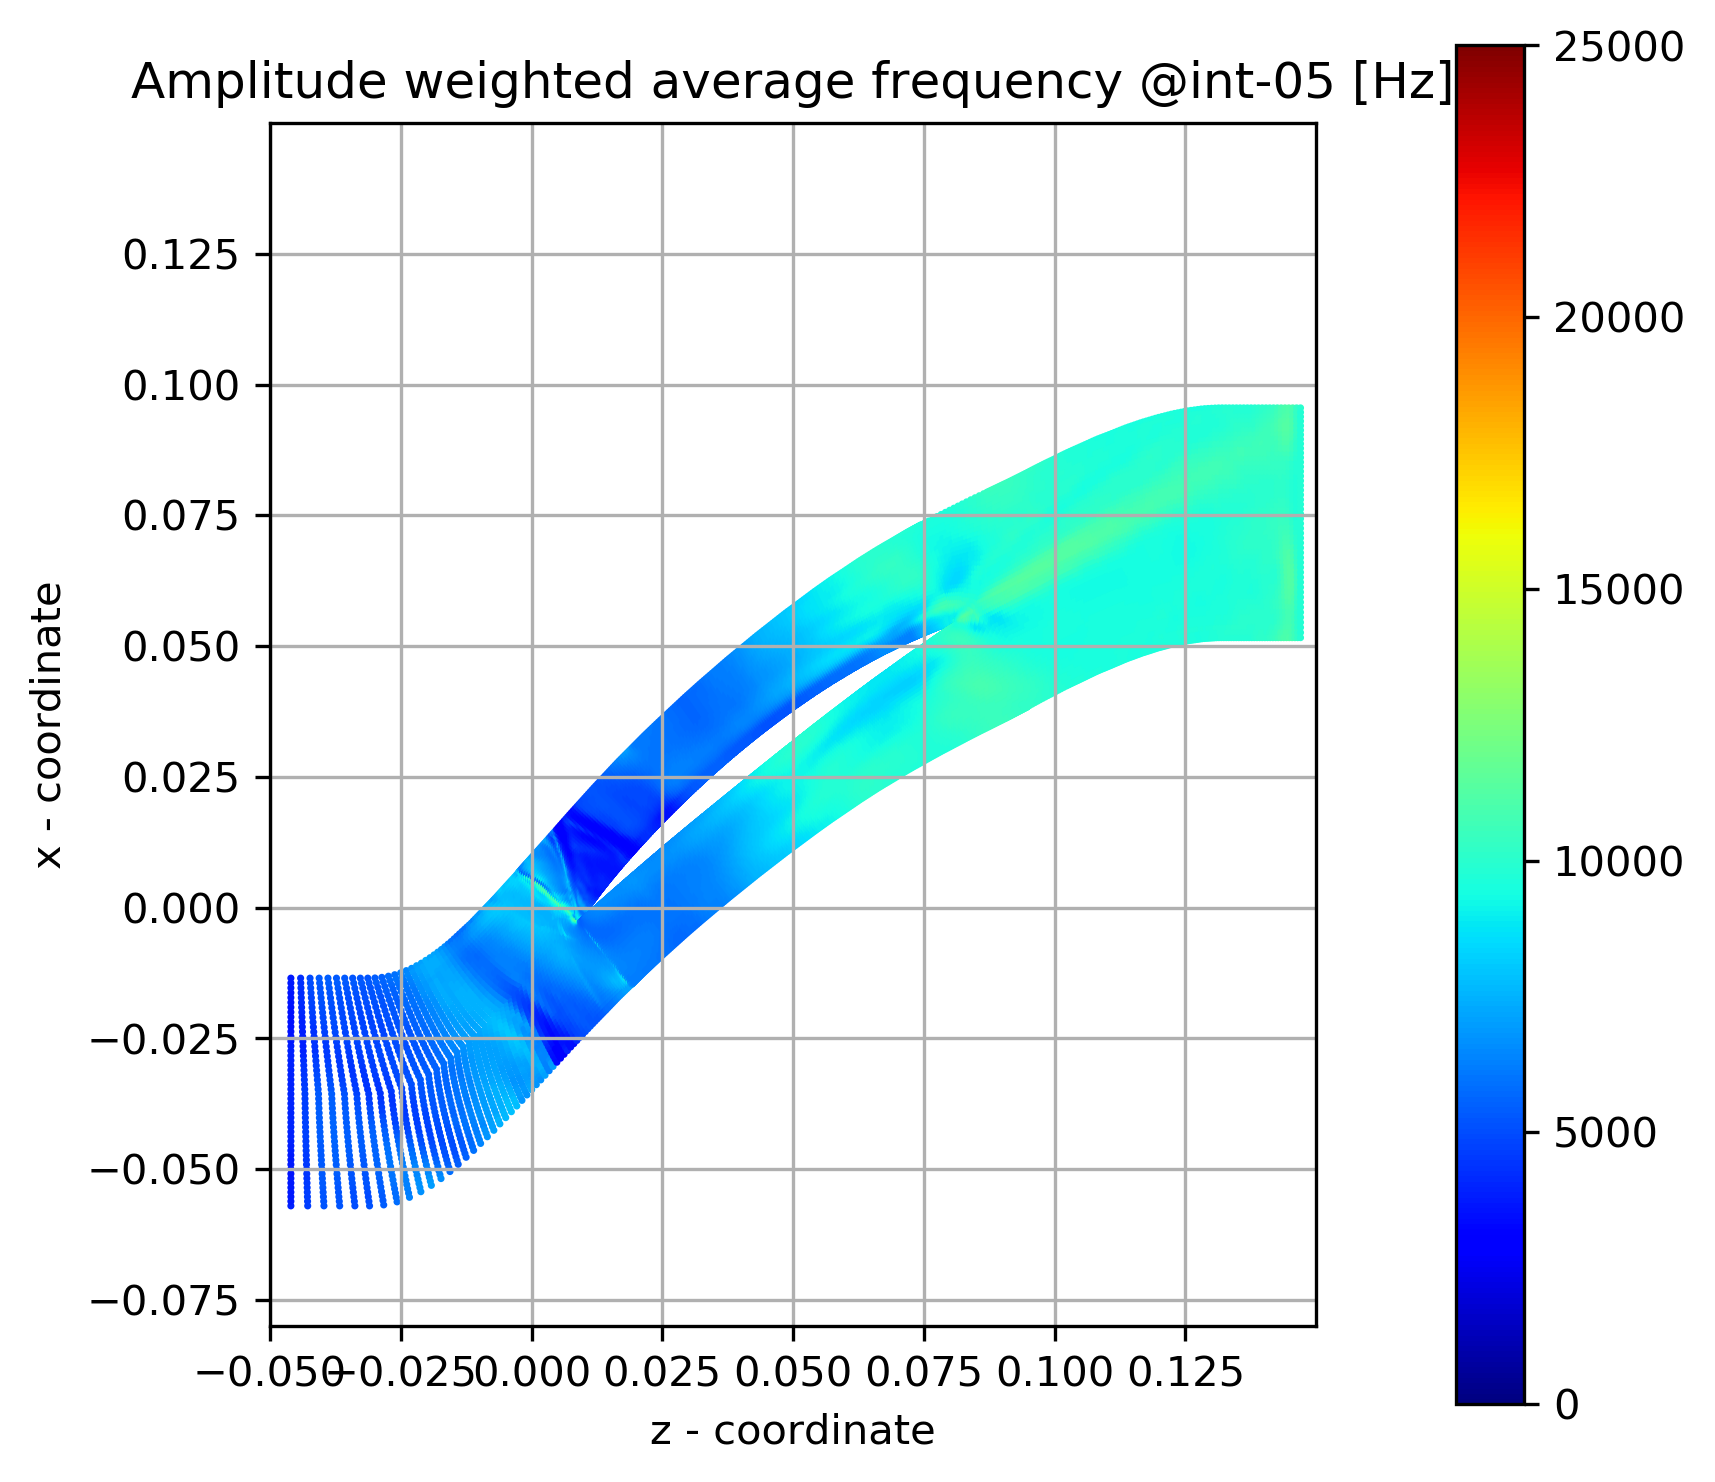
\includegraphics[width=0.75\textwidth]{Figures/int-05-awaf.png}
  \caption{Amplitude weighted average frequency at int-05 mark} \label{int-05-awaf}
\end{figure}
%int-05
\begin{figure}[ht]
  \centering
  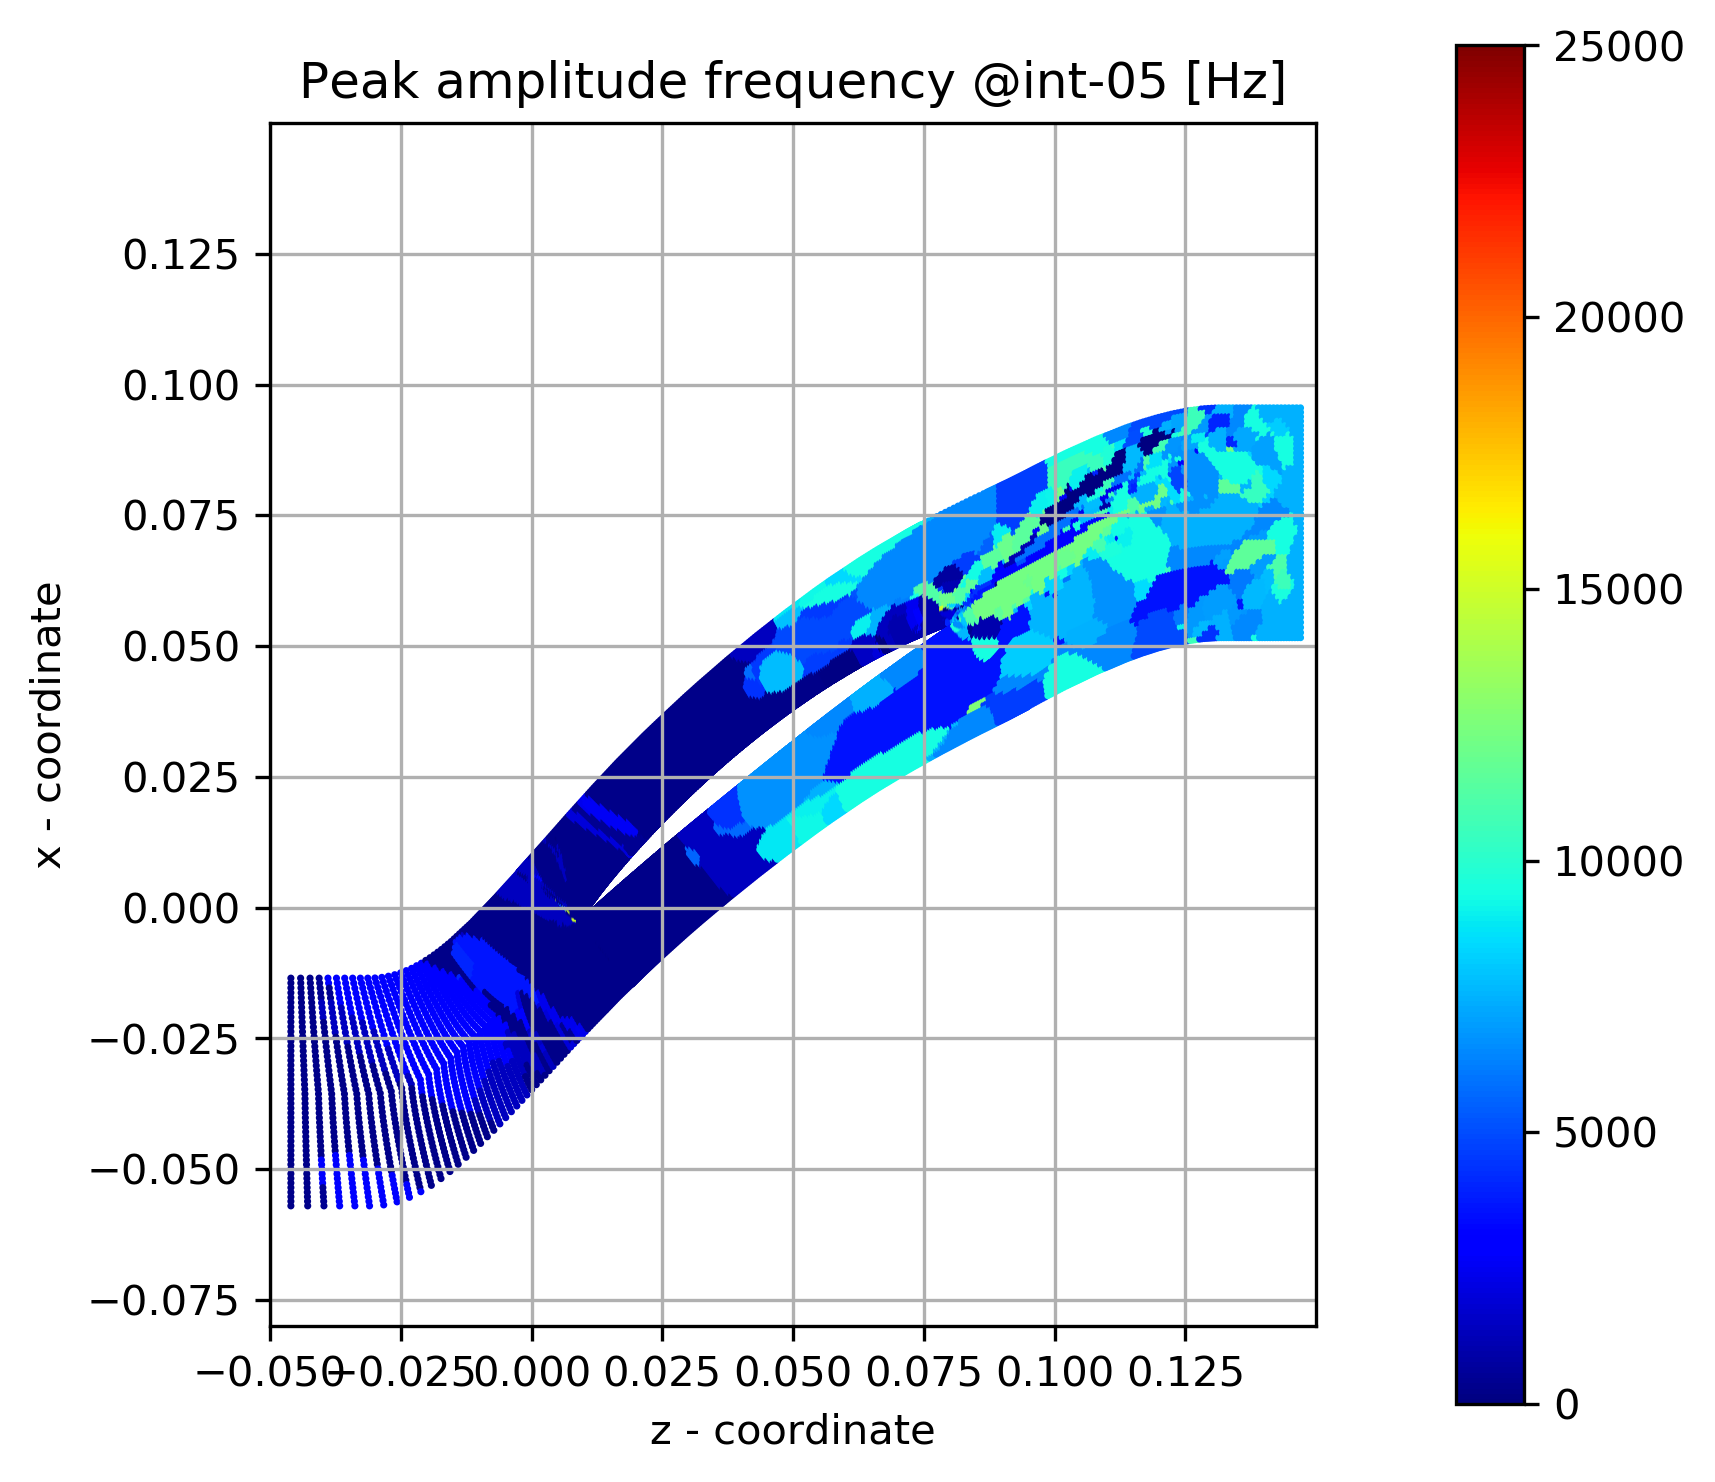
\includegraphics[width=0.75\textwidth]{Figures/int-05-peak-freq.png}
  \caption{Peak amplitude frequency int-05 mark} \label{int-05-peak-freq}
  
  \vspace*{\floatsep}% https://tex.stackexchange.com/q/26521/5764

  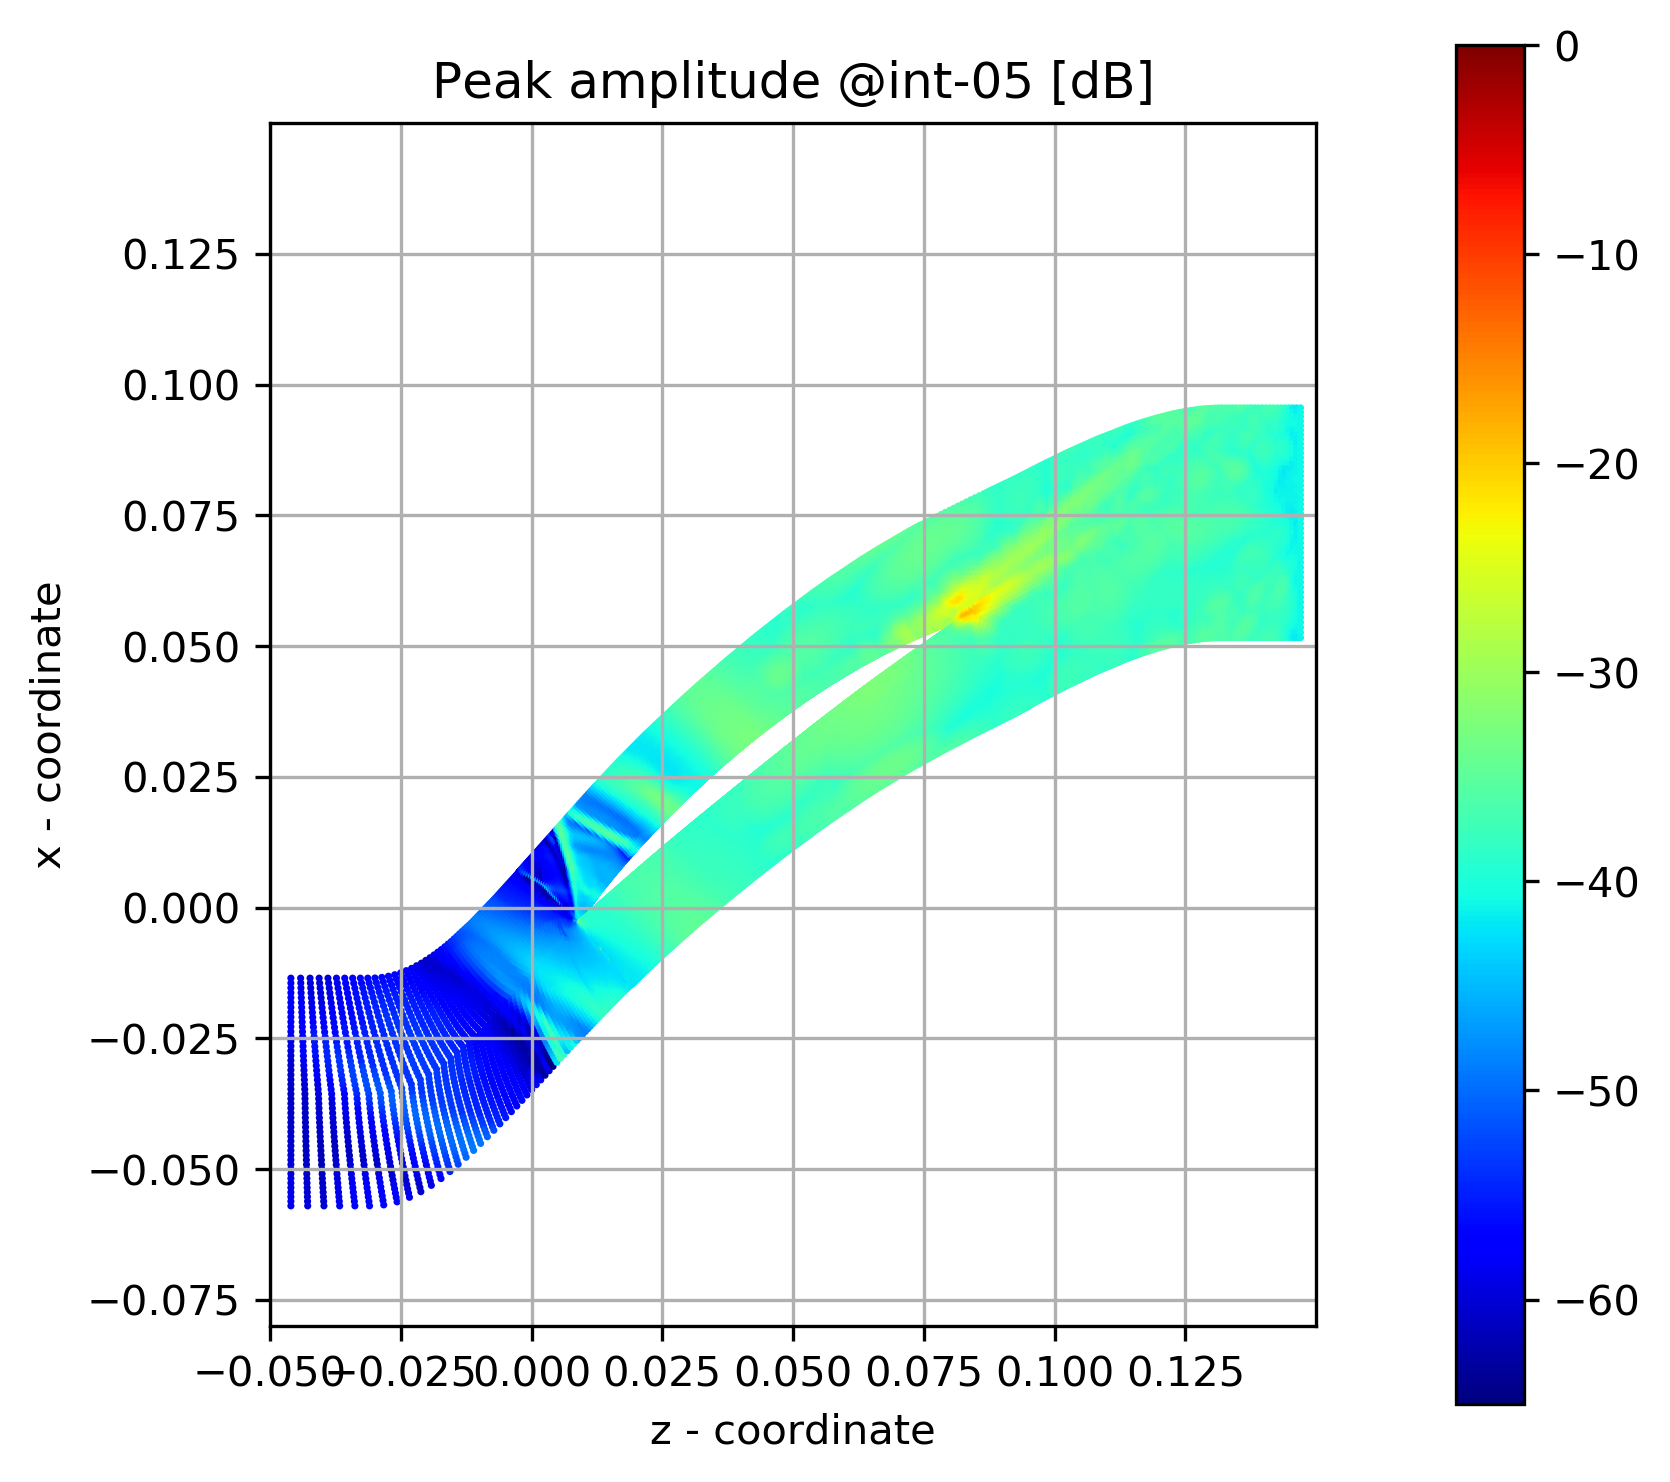
\includegraphics[width=0.75\textwidth]{Figures/int-05-peak-mag.png}
  \caption{Peak magnitude at int-05 mark} \label{int-05-peak-mag}
\end{figure}

%int-06
\begin{figure}[ht]
  \centering
  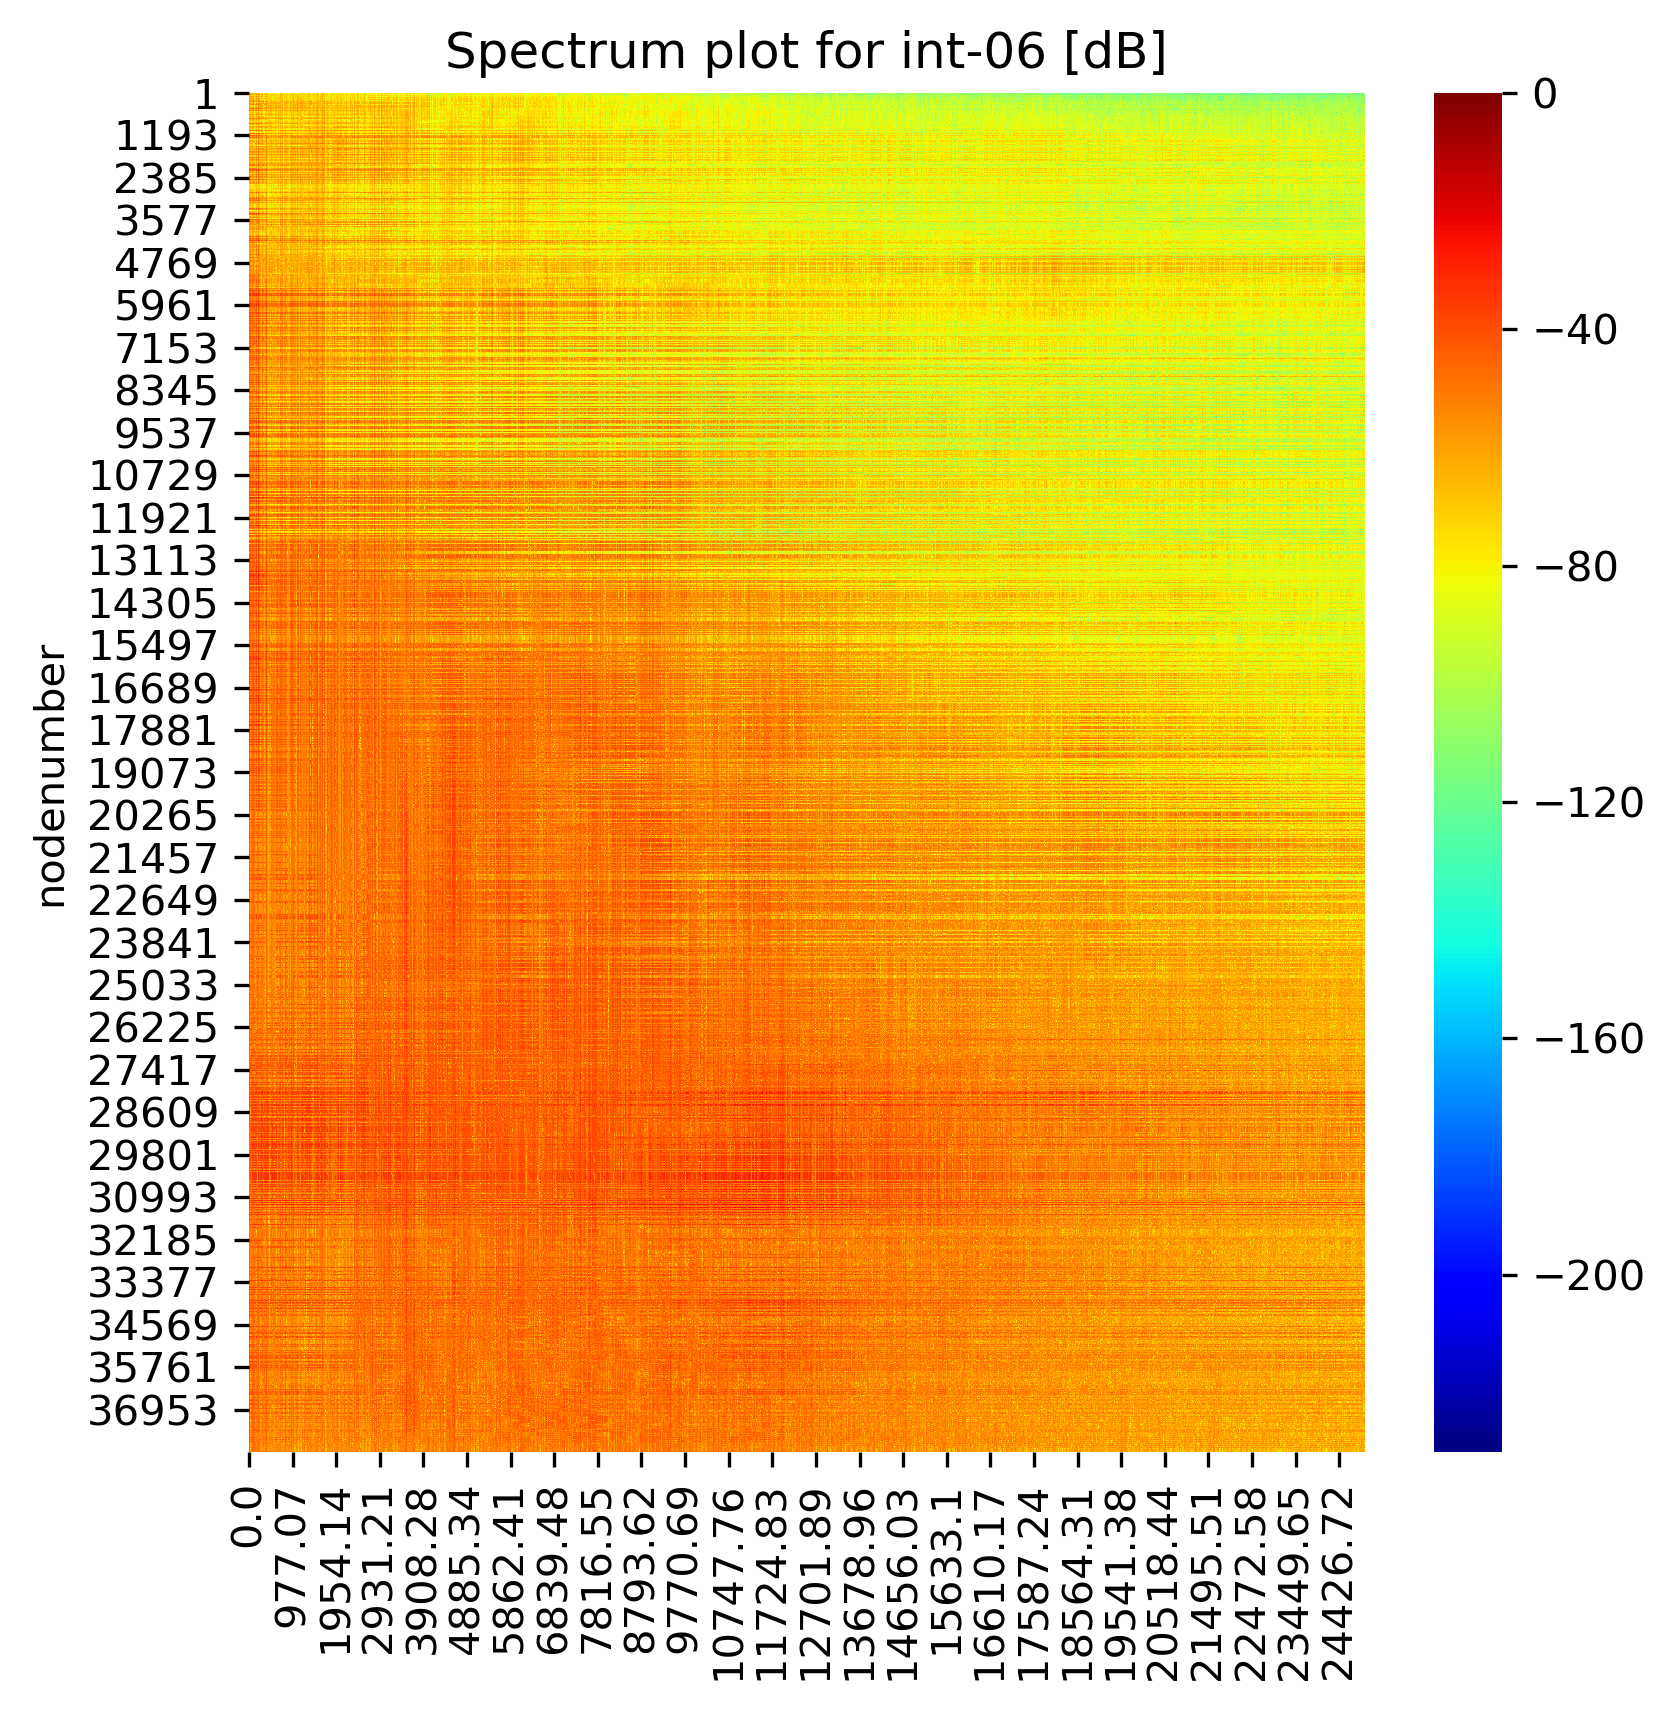
\includegraphics[width=0.75\textwidth]{Figures/int-06_spectrum.png}
  \caption{Spectrum plot at int-06 mark} \label{int-06-spectrum}
  
  \vspace*{\floatsep}% https://tex.stackexchange.com/q/26521/5764

  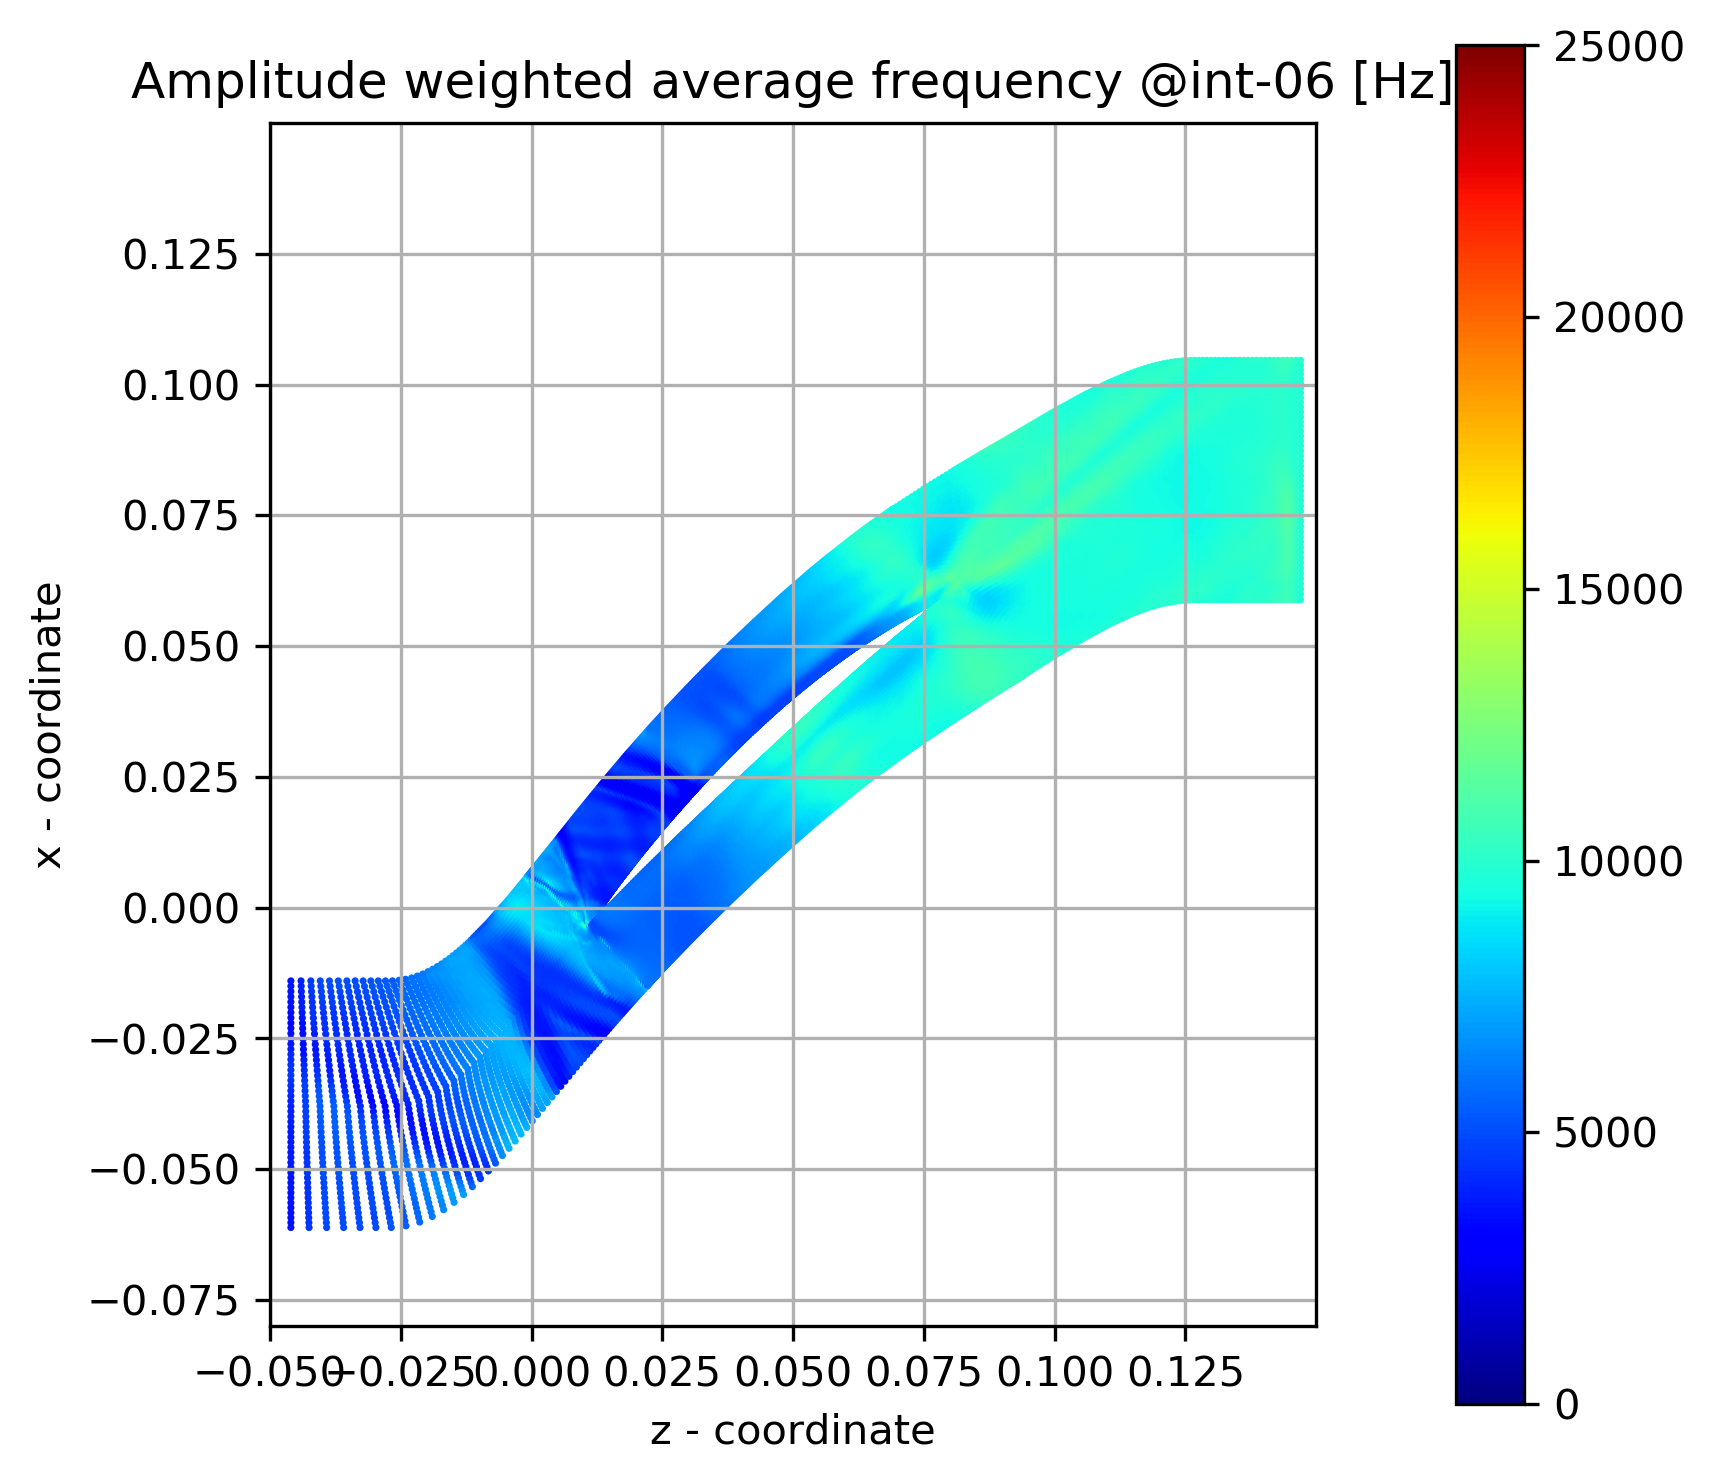
\includegraphics[width=0.75\textwidth]{Figures/int-06-awaf.png}
  \caption{Amplitude weighted average frequency at int-06 mark} \label{int-06-awaf}
\end{figure}
%int-06
\begin{figure}[ht]
  \centering
  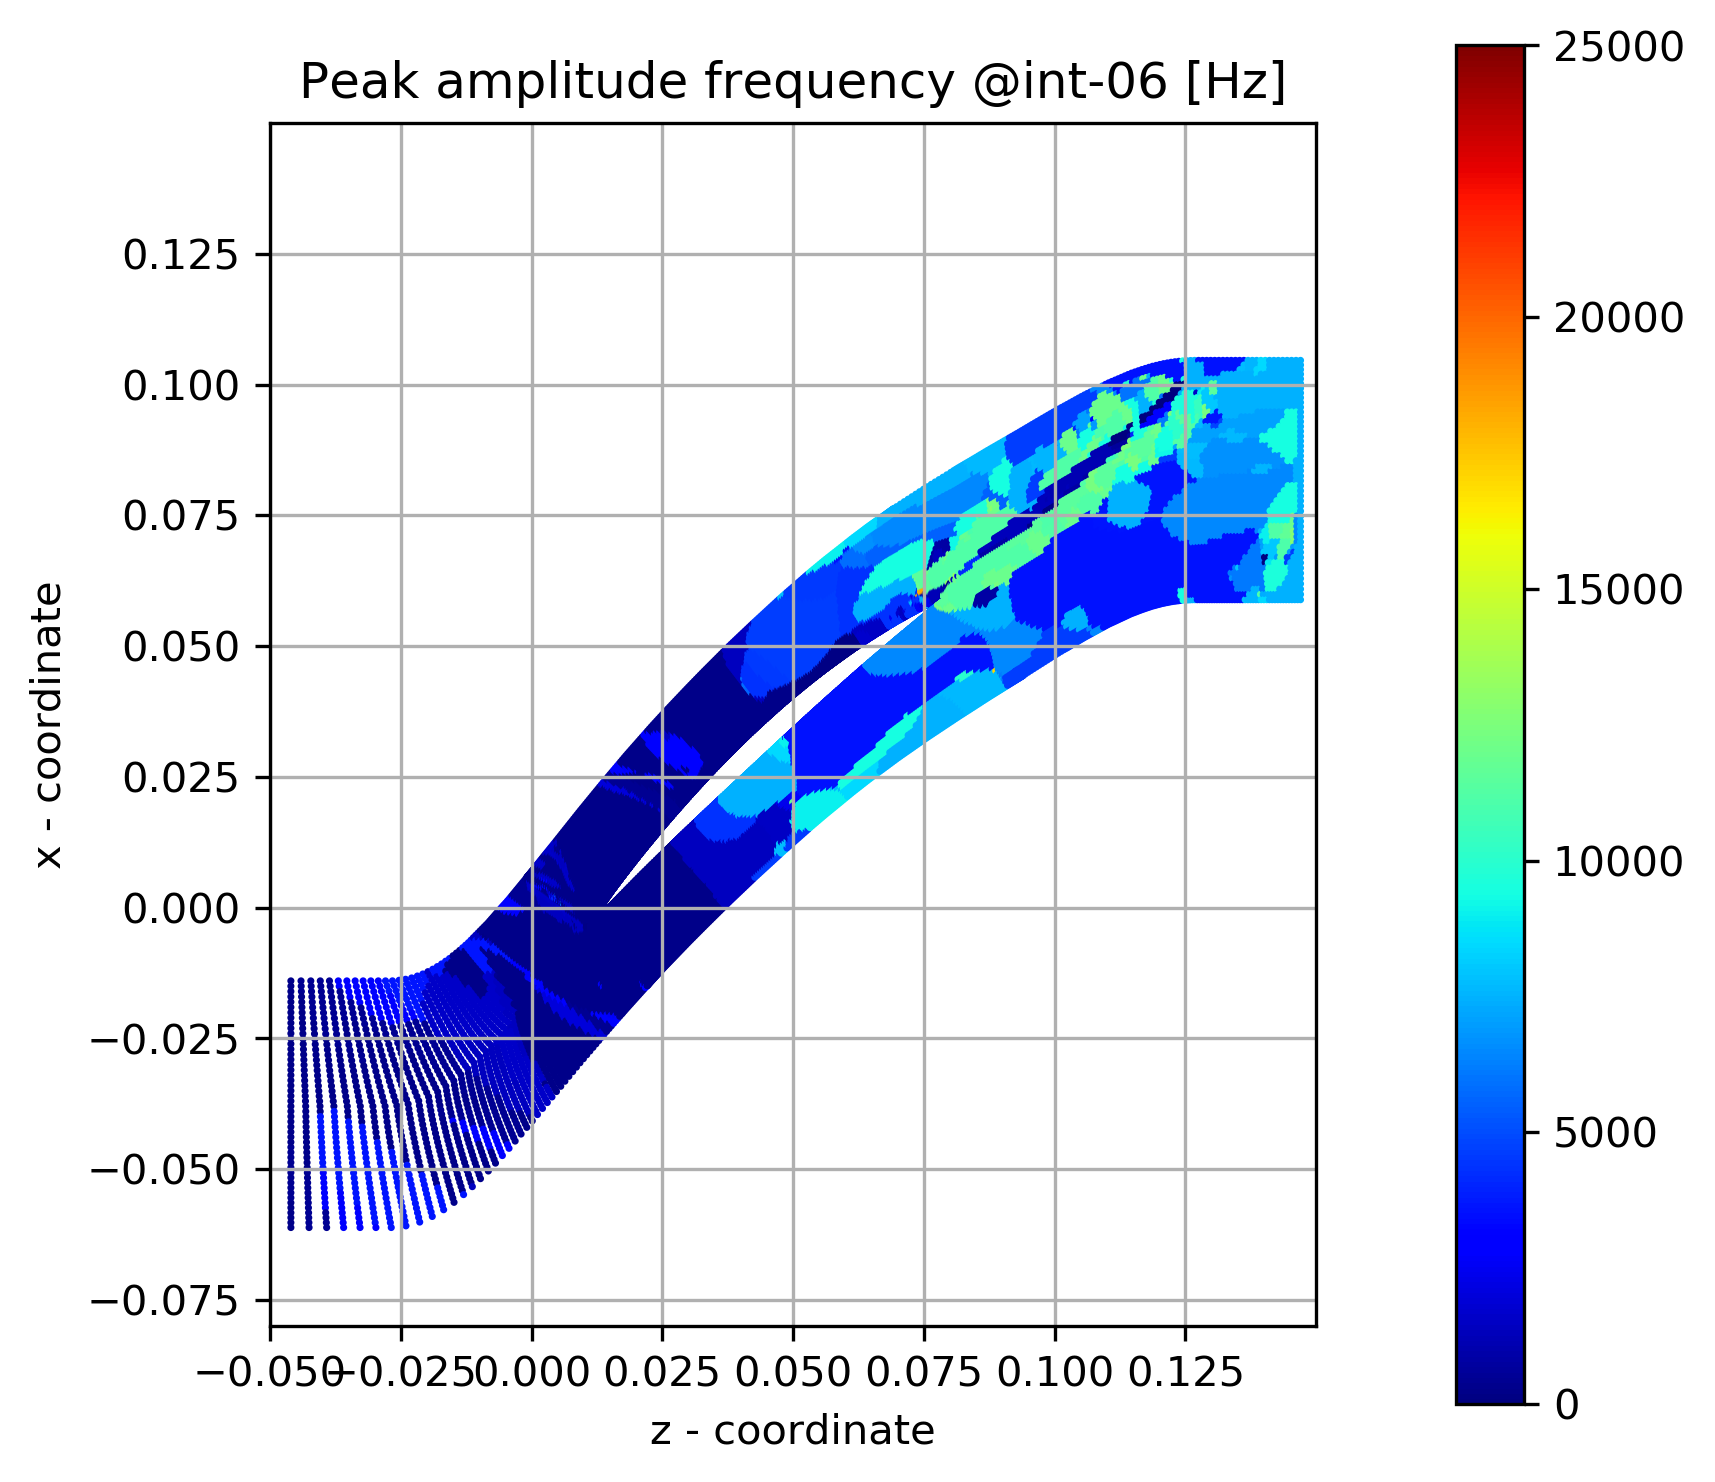
\includegraphics[width=0.75\textwidth]{Figures/int-06-peak-freq.png}
  \caption{Peak amplitude frequency int-06 mark} \label{int-06-peak-freq}
  
  \vspace*{\floatsep}% https://tex.stackexchange.com/q/26521/5764

  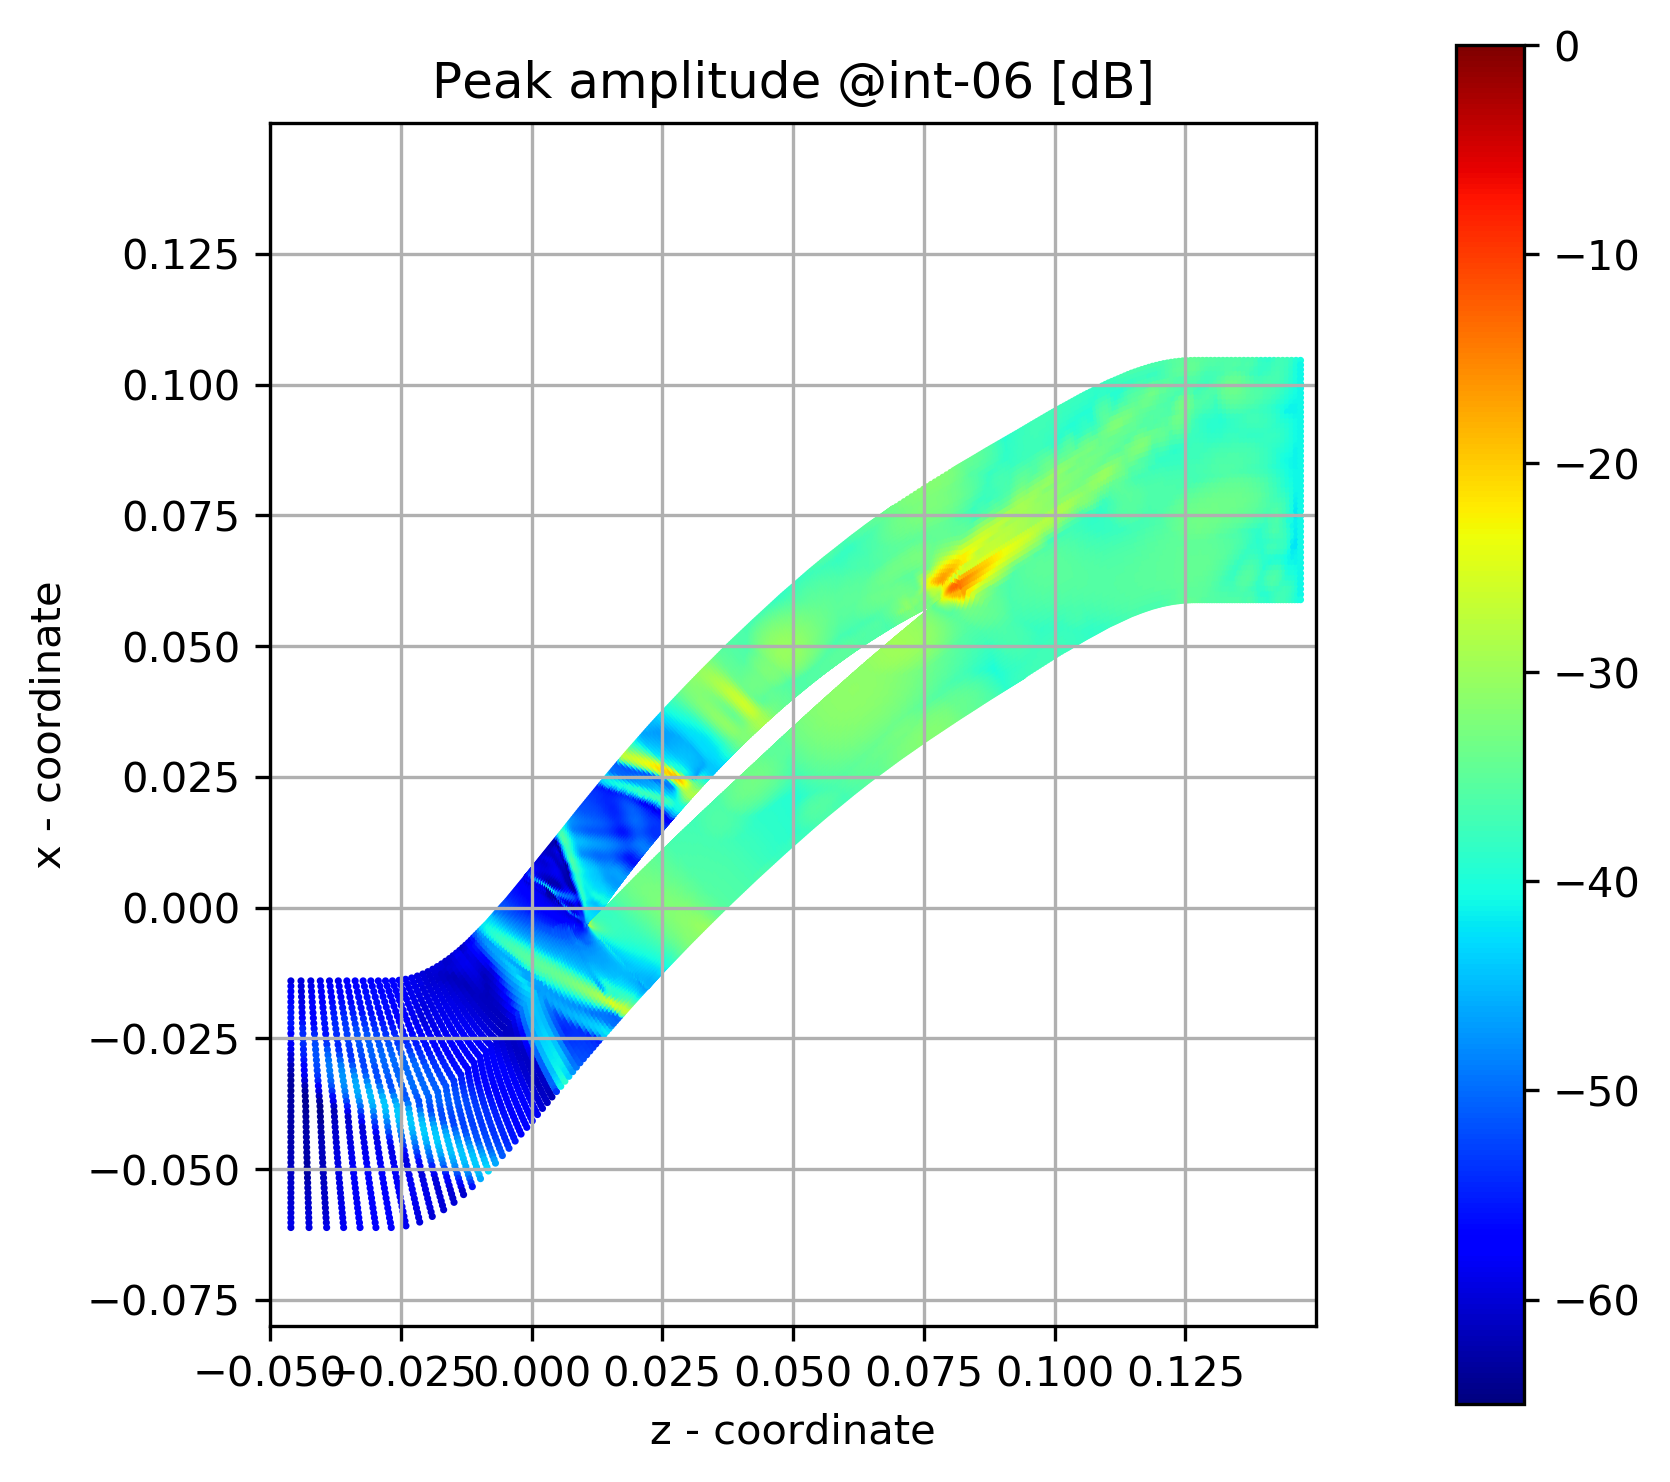
\includegraphics[width=0.75\textwidth]{Figures/int-06-peak-mag.png}
  \caption{Peak magnitude at int-06 mark} \label{int-06-peak-mag}
\end{figure}

%int-07
\begin{figure}[ht]
  \centering
  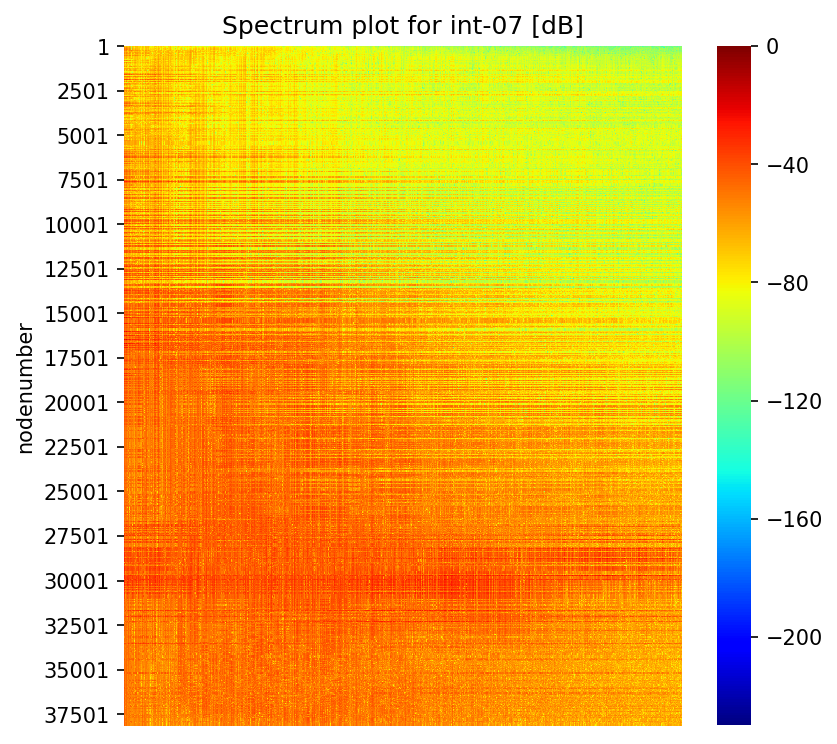
\includegraphics[width=0.75\textwidth]{Figures/int-07_spectrum.png}
  \caption{Spectrum plot at int-07 mark} \label{int-07-spectrum}
  
  \vspace*{\floatsep}% https://tex.stackexchange.com/q/26521/5764

  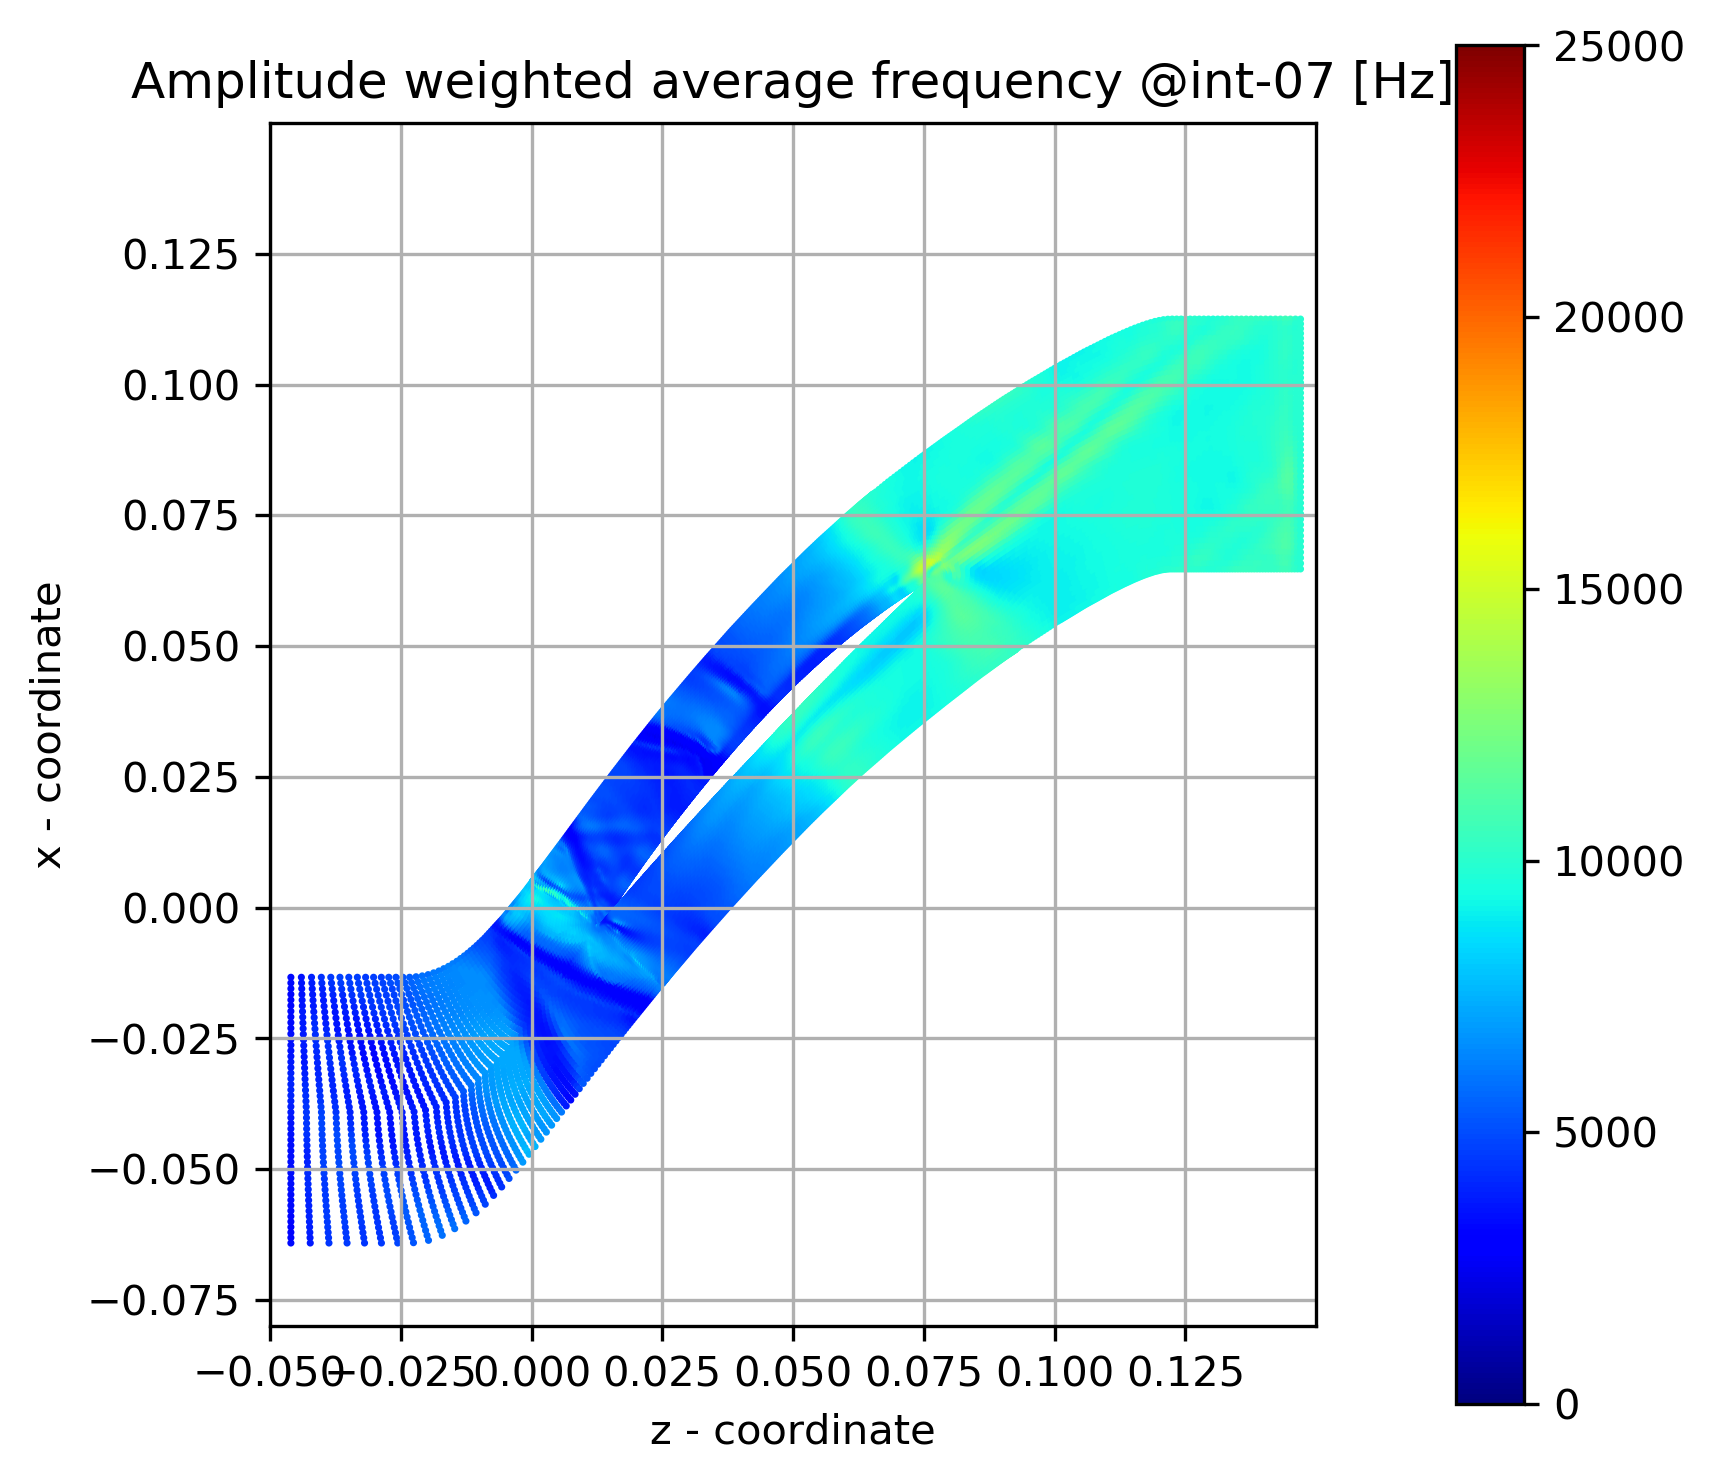
\includegraphics[width=0.75\textwidth]{Figures/int-07-awaf.png}
  \caption{Amplitude weighted average frequency at int-07 mark} \label{int-07-awaf}
\end{figure}
%int-07
\begin{figure}[ht]
  \centering
  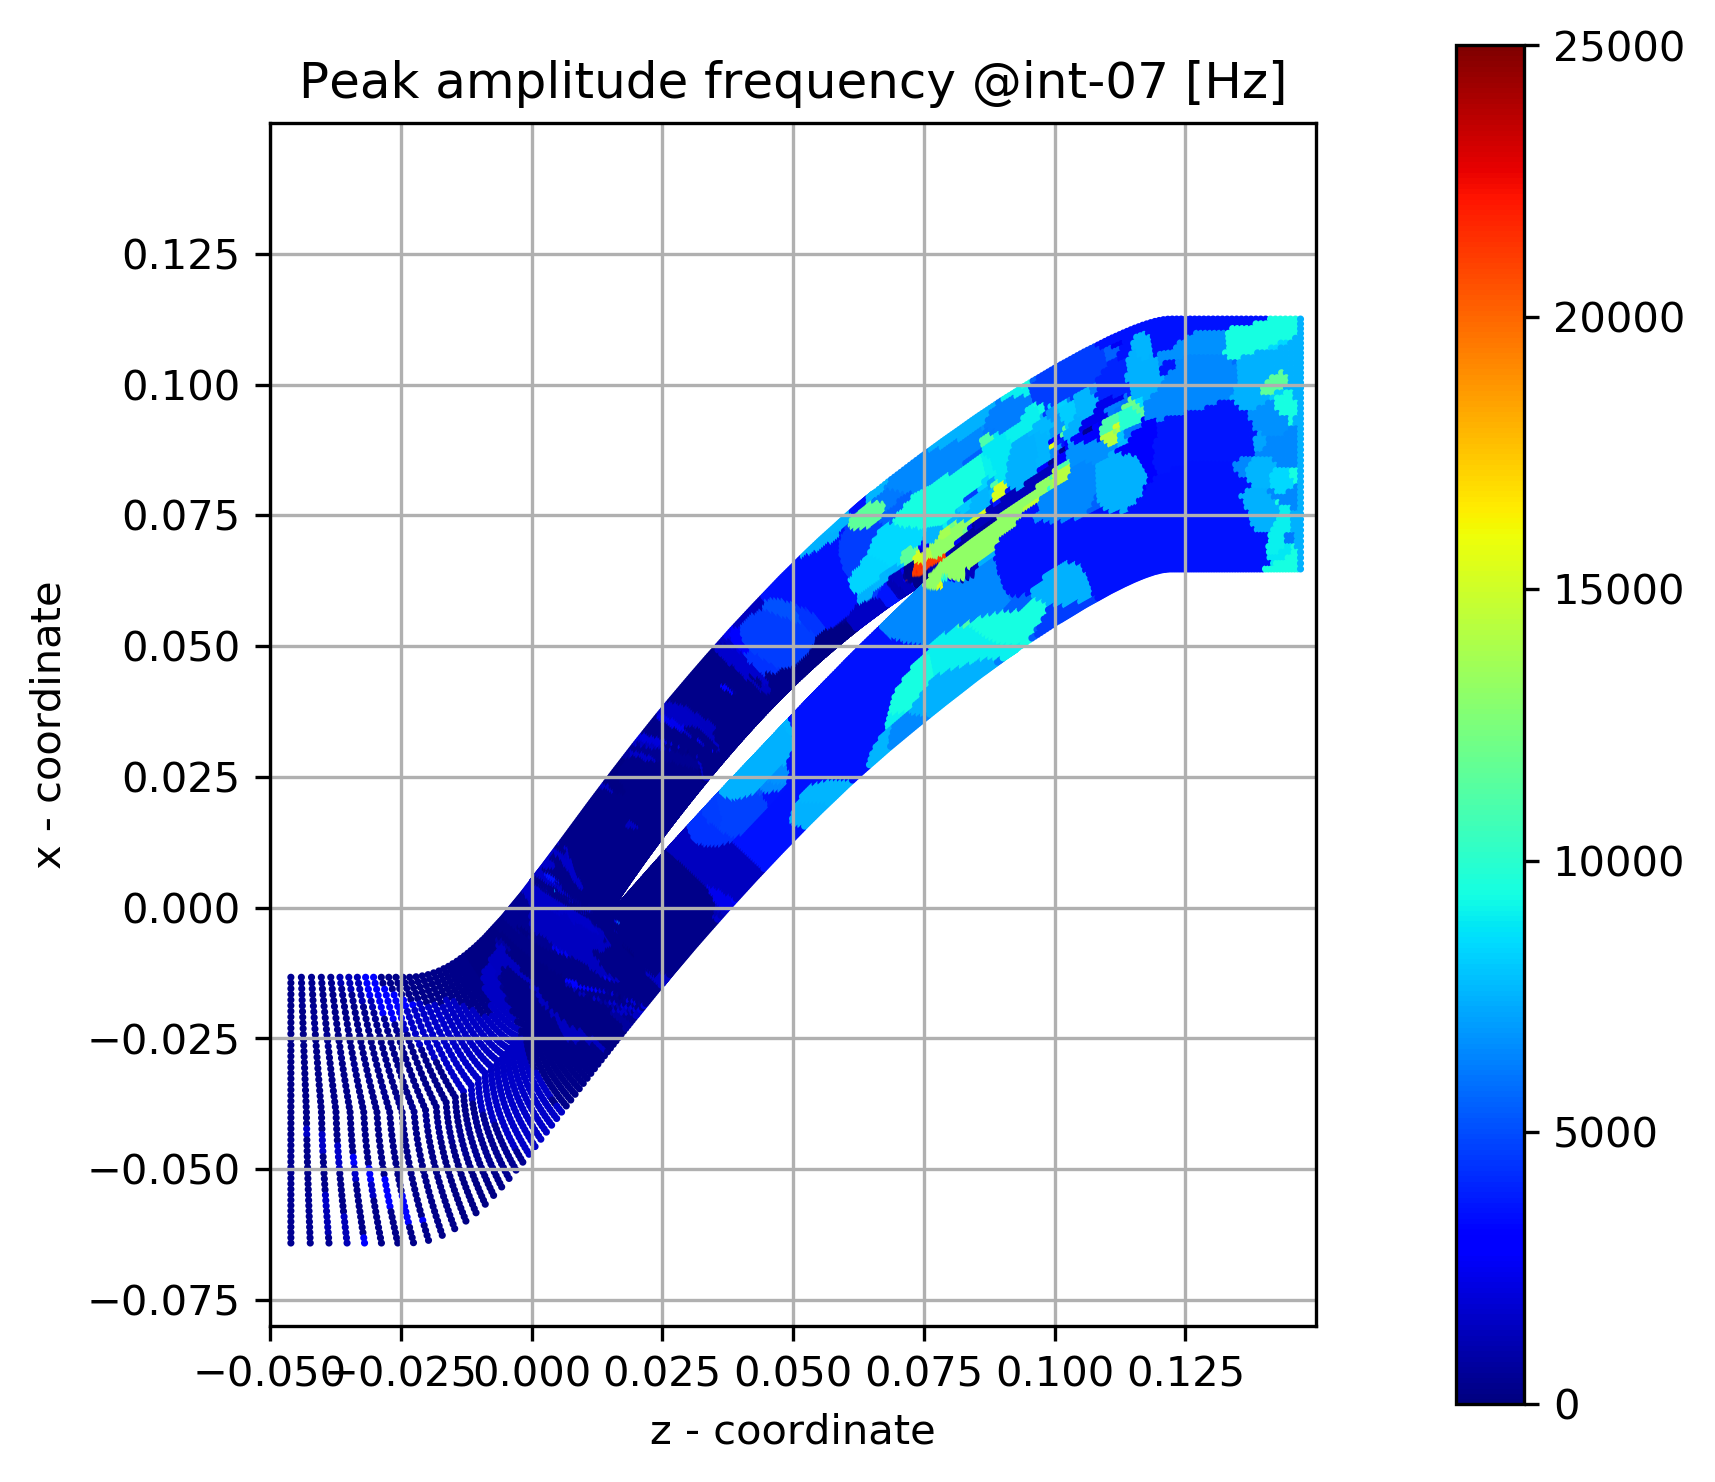
\includegraphics[width=0.75\textwidth]{Figures/int-07-peak-freq.png}
  \caption{Peak amplitude frequency int-07 mark} \label{int-07-peak-freq}
  
  \vspace*{\floatsep}% https://tex.stackexchange.com/q/26521/5764

  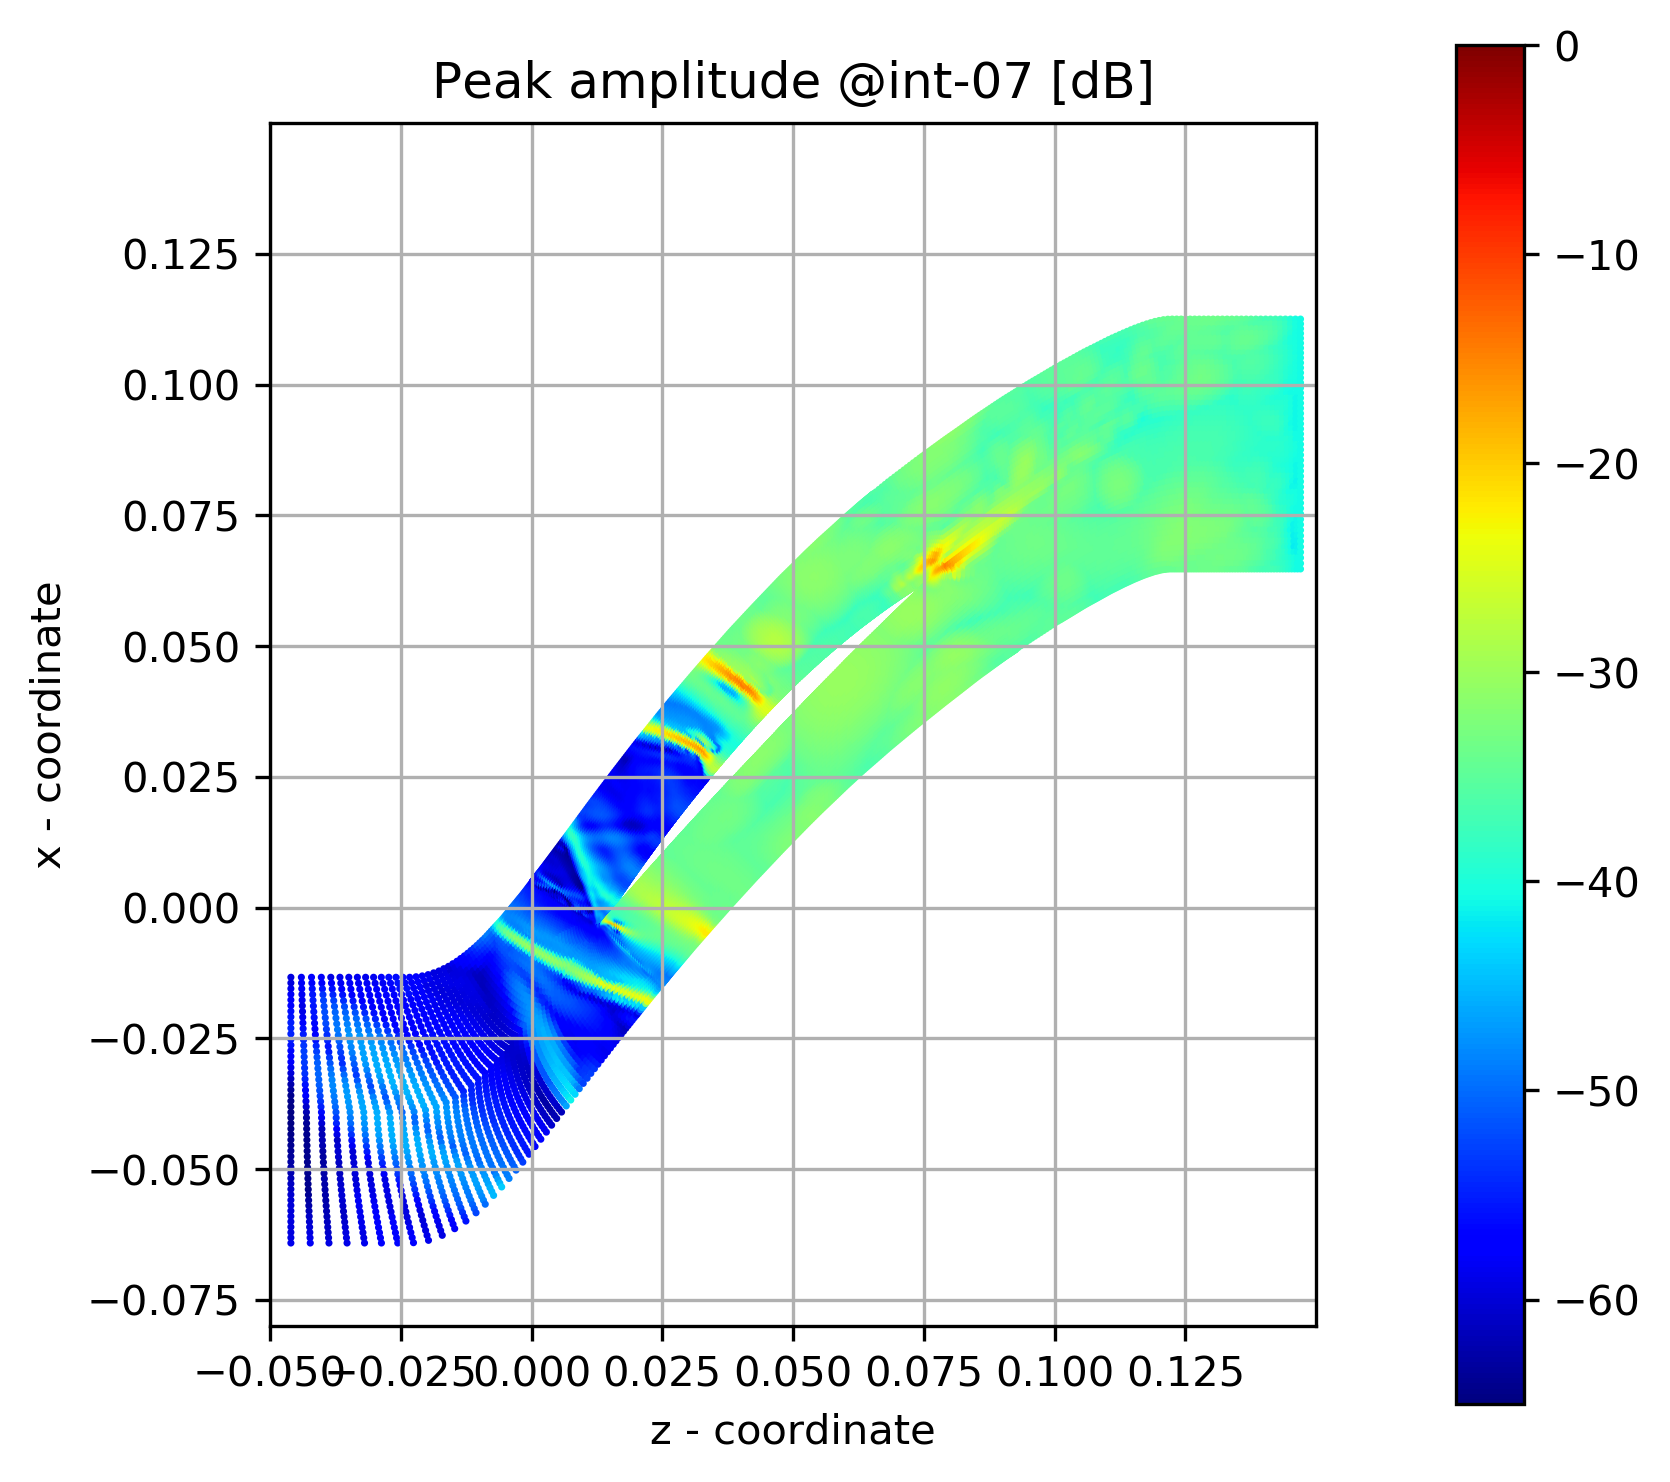
\includegraphics[width=0.75\textwidth]{Figures/int-07-peak-mag.png}
  \caption{Peak magnitude at int-07 mark} \label{int-07-peak-mag}
\end{figure}

%int-08
\begin{figure}[ht]
  \centering
  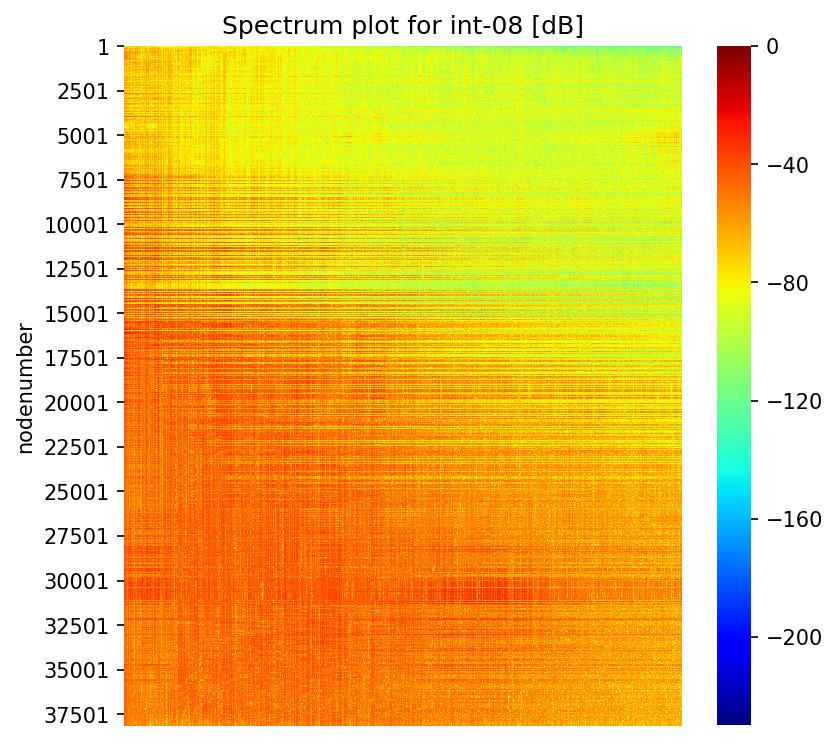
\includegraphics[width=0.75\textwidth]{Figures/int-08_spectrum.png}
  \caption{Spectrum plot at int-08 mark} \label{int-08-spectrum}
  
  \vspace*{\floatsep}% https://tex.stackexchange.com/q/26521/5764

  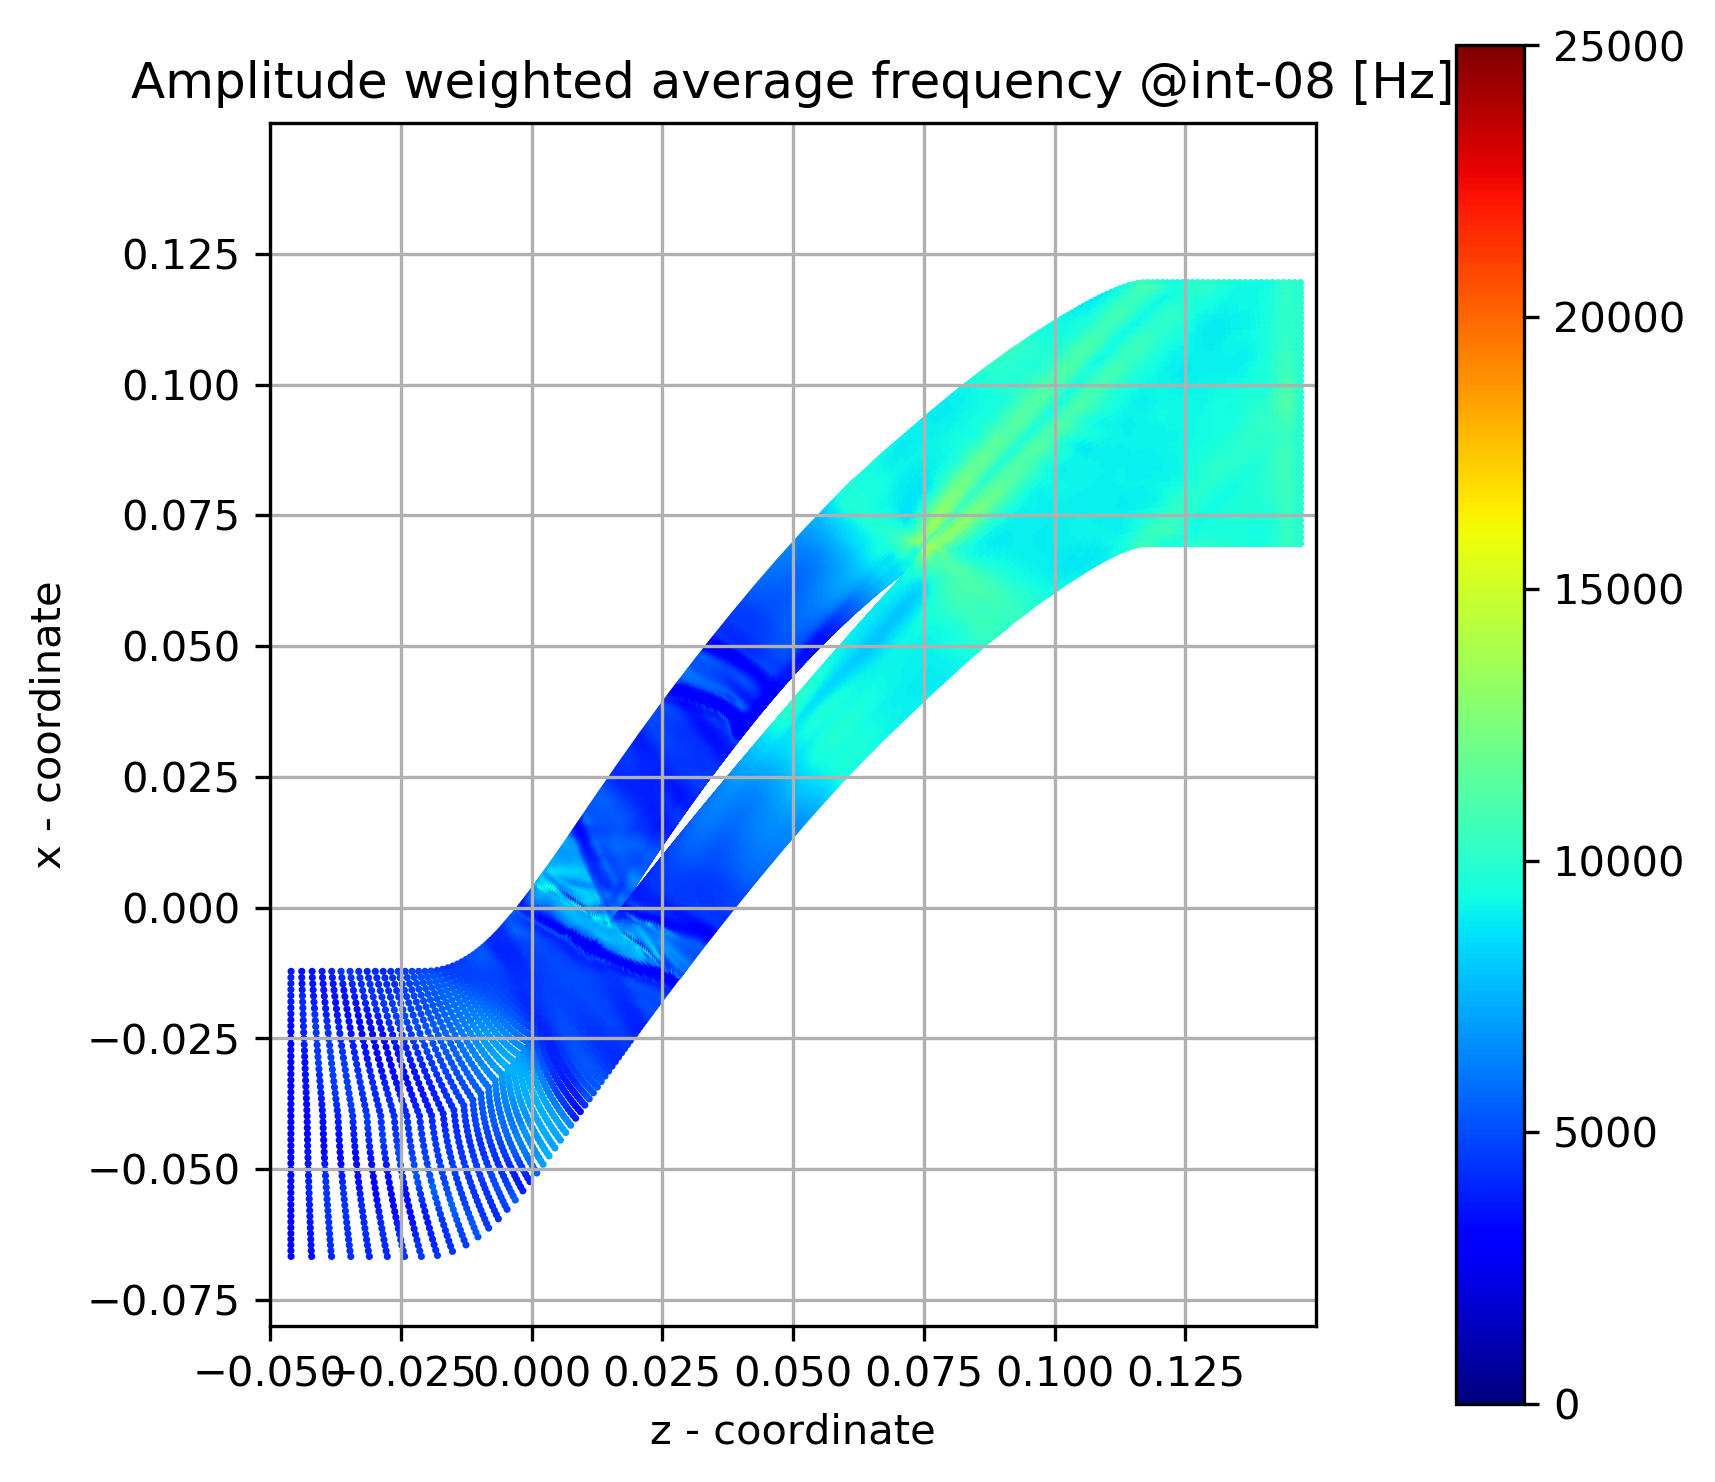
\includegraphics[width=0.75\textwidth]{Figures/int-08-awaf.png}
  \caption{Amplitude weighted average frequency at int-08 mark} \label{int-08-awaf}
\end{figure}
%int-08
\begin{figure}[ht]
  \centering
  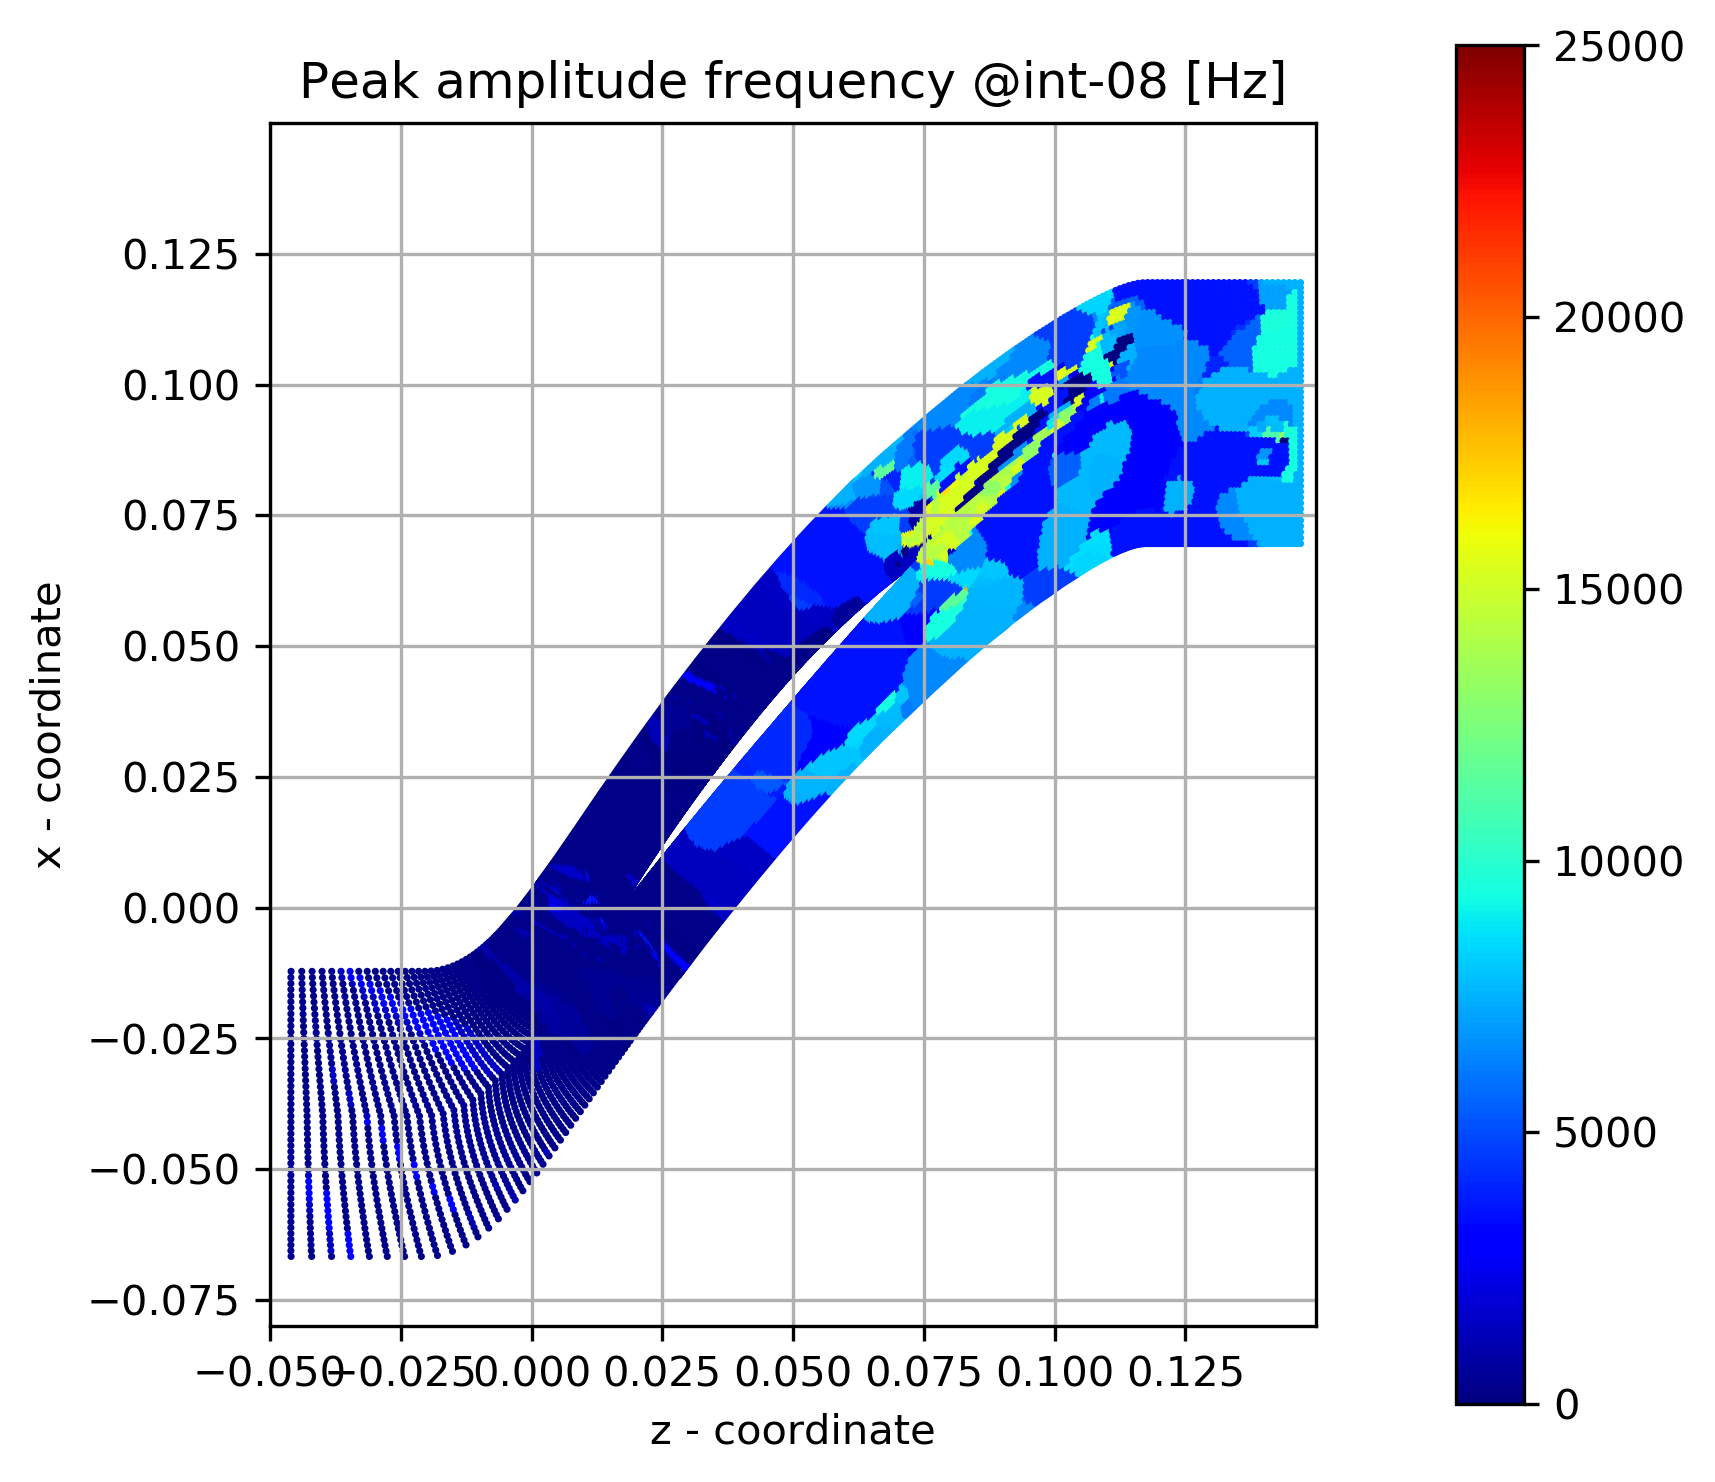
\includegraphics[width=0.75\textwidth]{Figures/int-08-peak-freq.png}
  \caption{Peak amplitude frequency int-08 mark} \label{int-08-peak-freq}
  
  \vspace*{\floatsep}% https://tex.stackexchange.com/q/26521/5764

  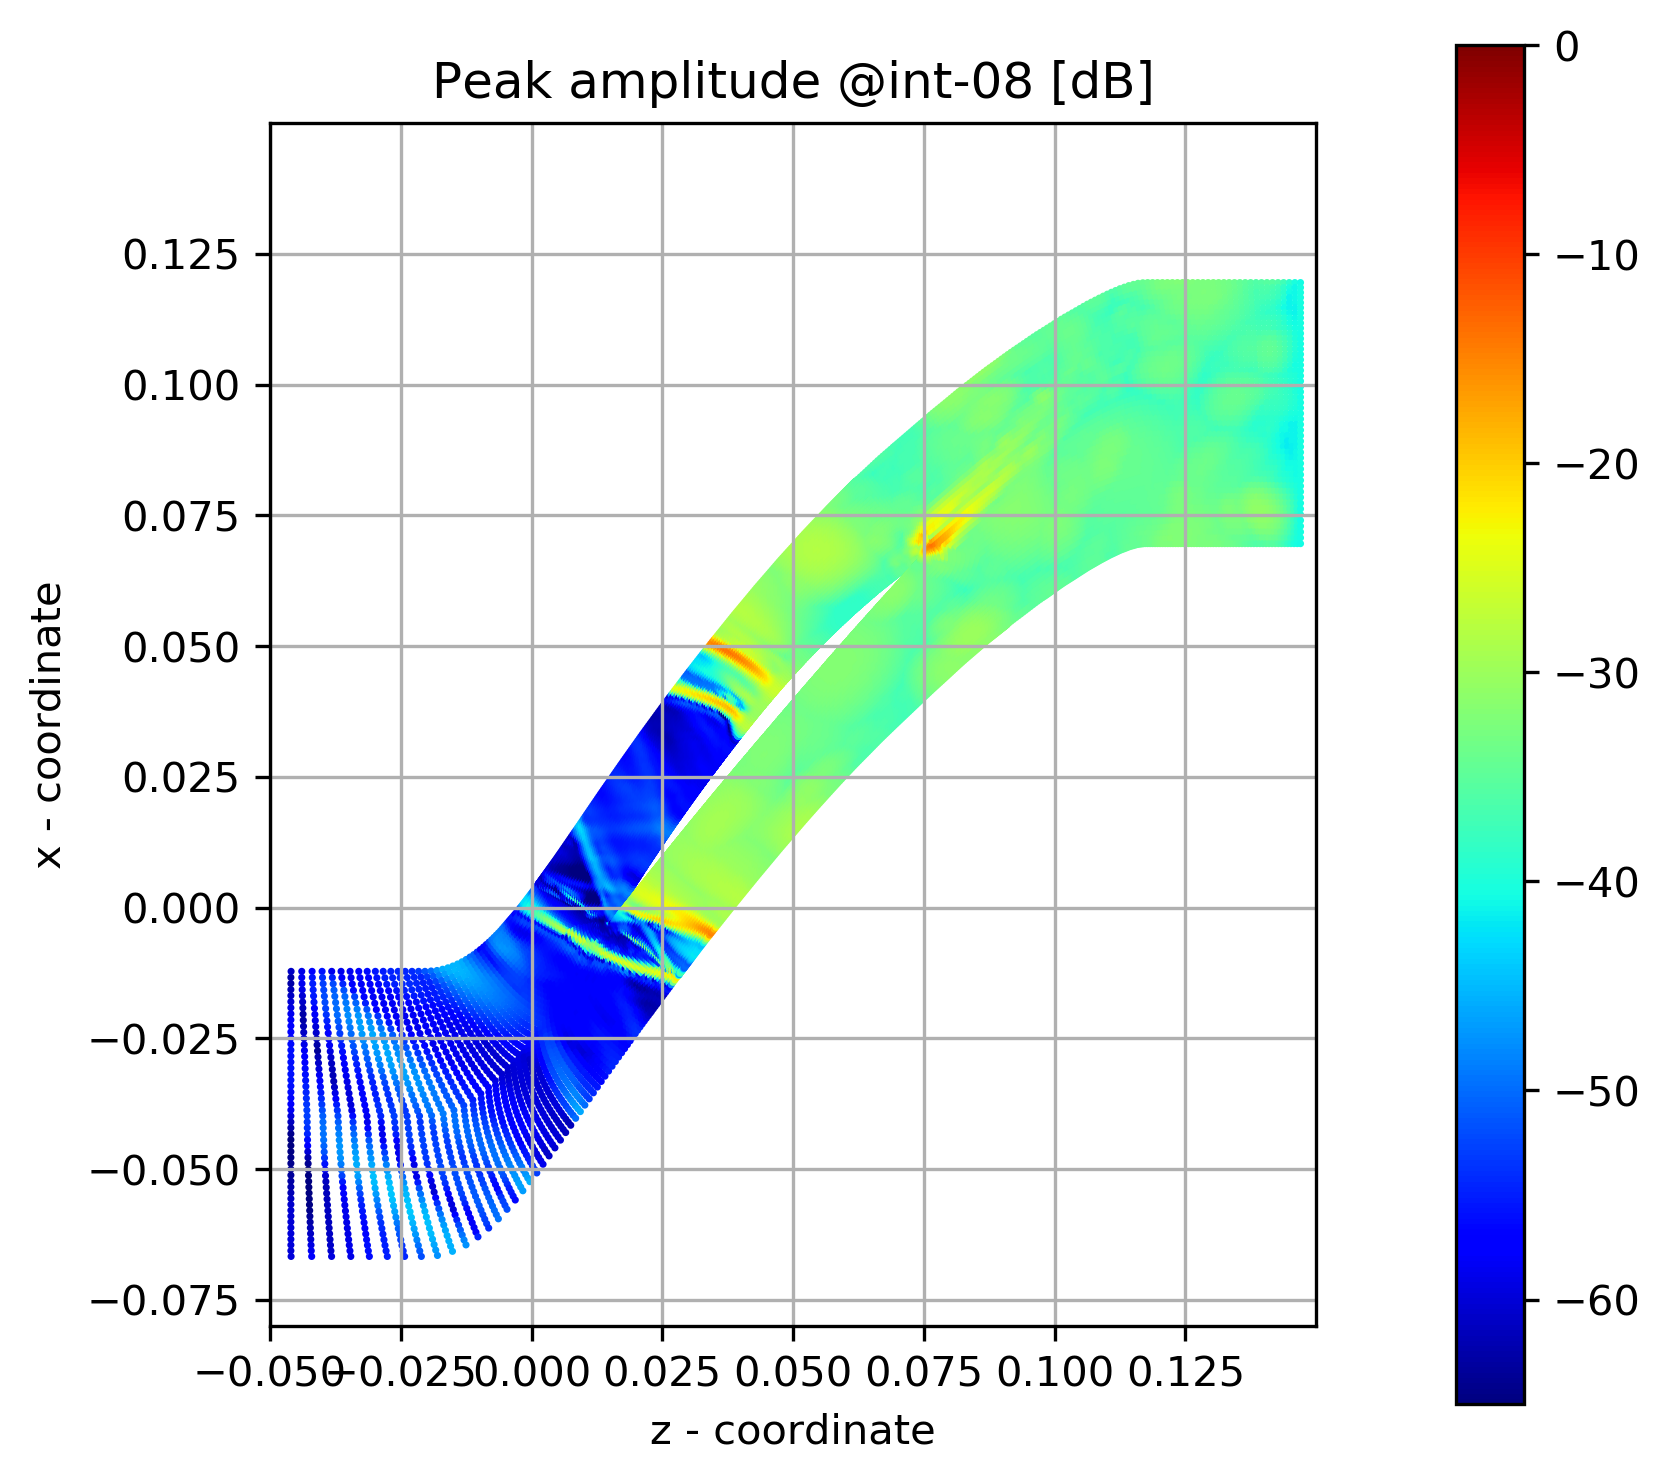
\includegraphics[width=0.75\textwidth]{Figures/int-08-peak-mag.png}
  \caption{Peak magnitude at int-08 mark} \label{int-08-peak-mag}
\end{figure}

%int-09
\begin{figure}[ht]
  \centering
  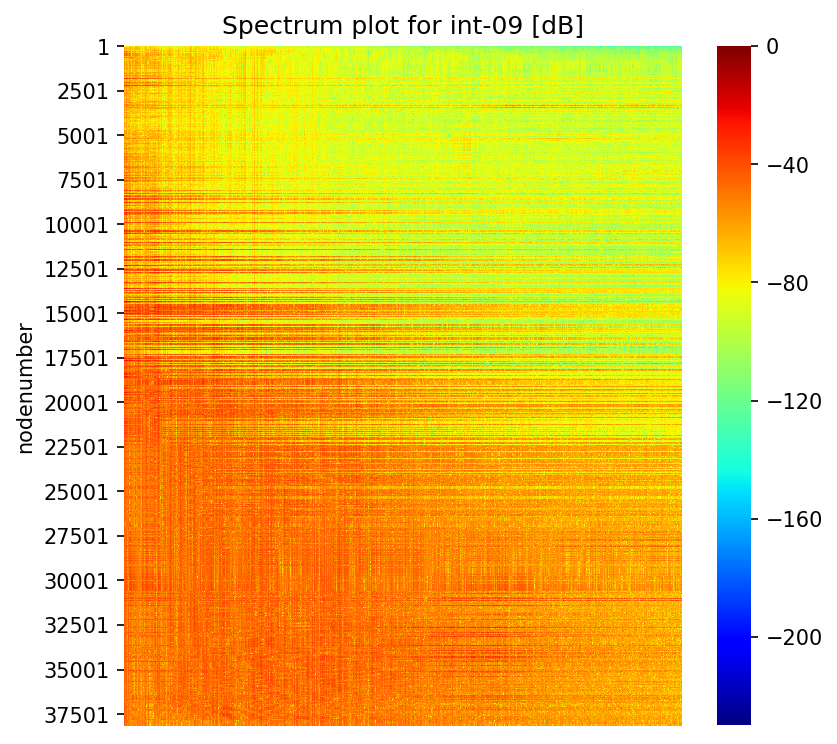
\includegraphics[width=0.75\textwidth]{Figures/int-09_spectrum.png}
  \caption{Spectrum plot at int-09 mark} \label{int-09-spectrum}
  
  \vspace*{\floatsep}% https://tex.stackexchange.com/q/26521/5764

  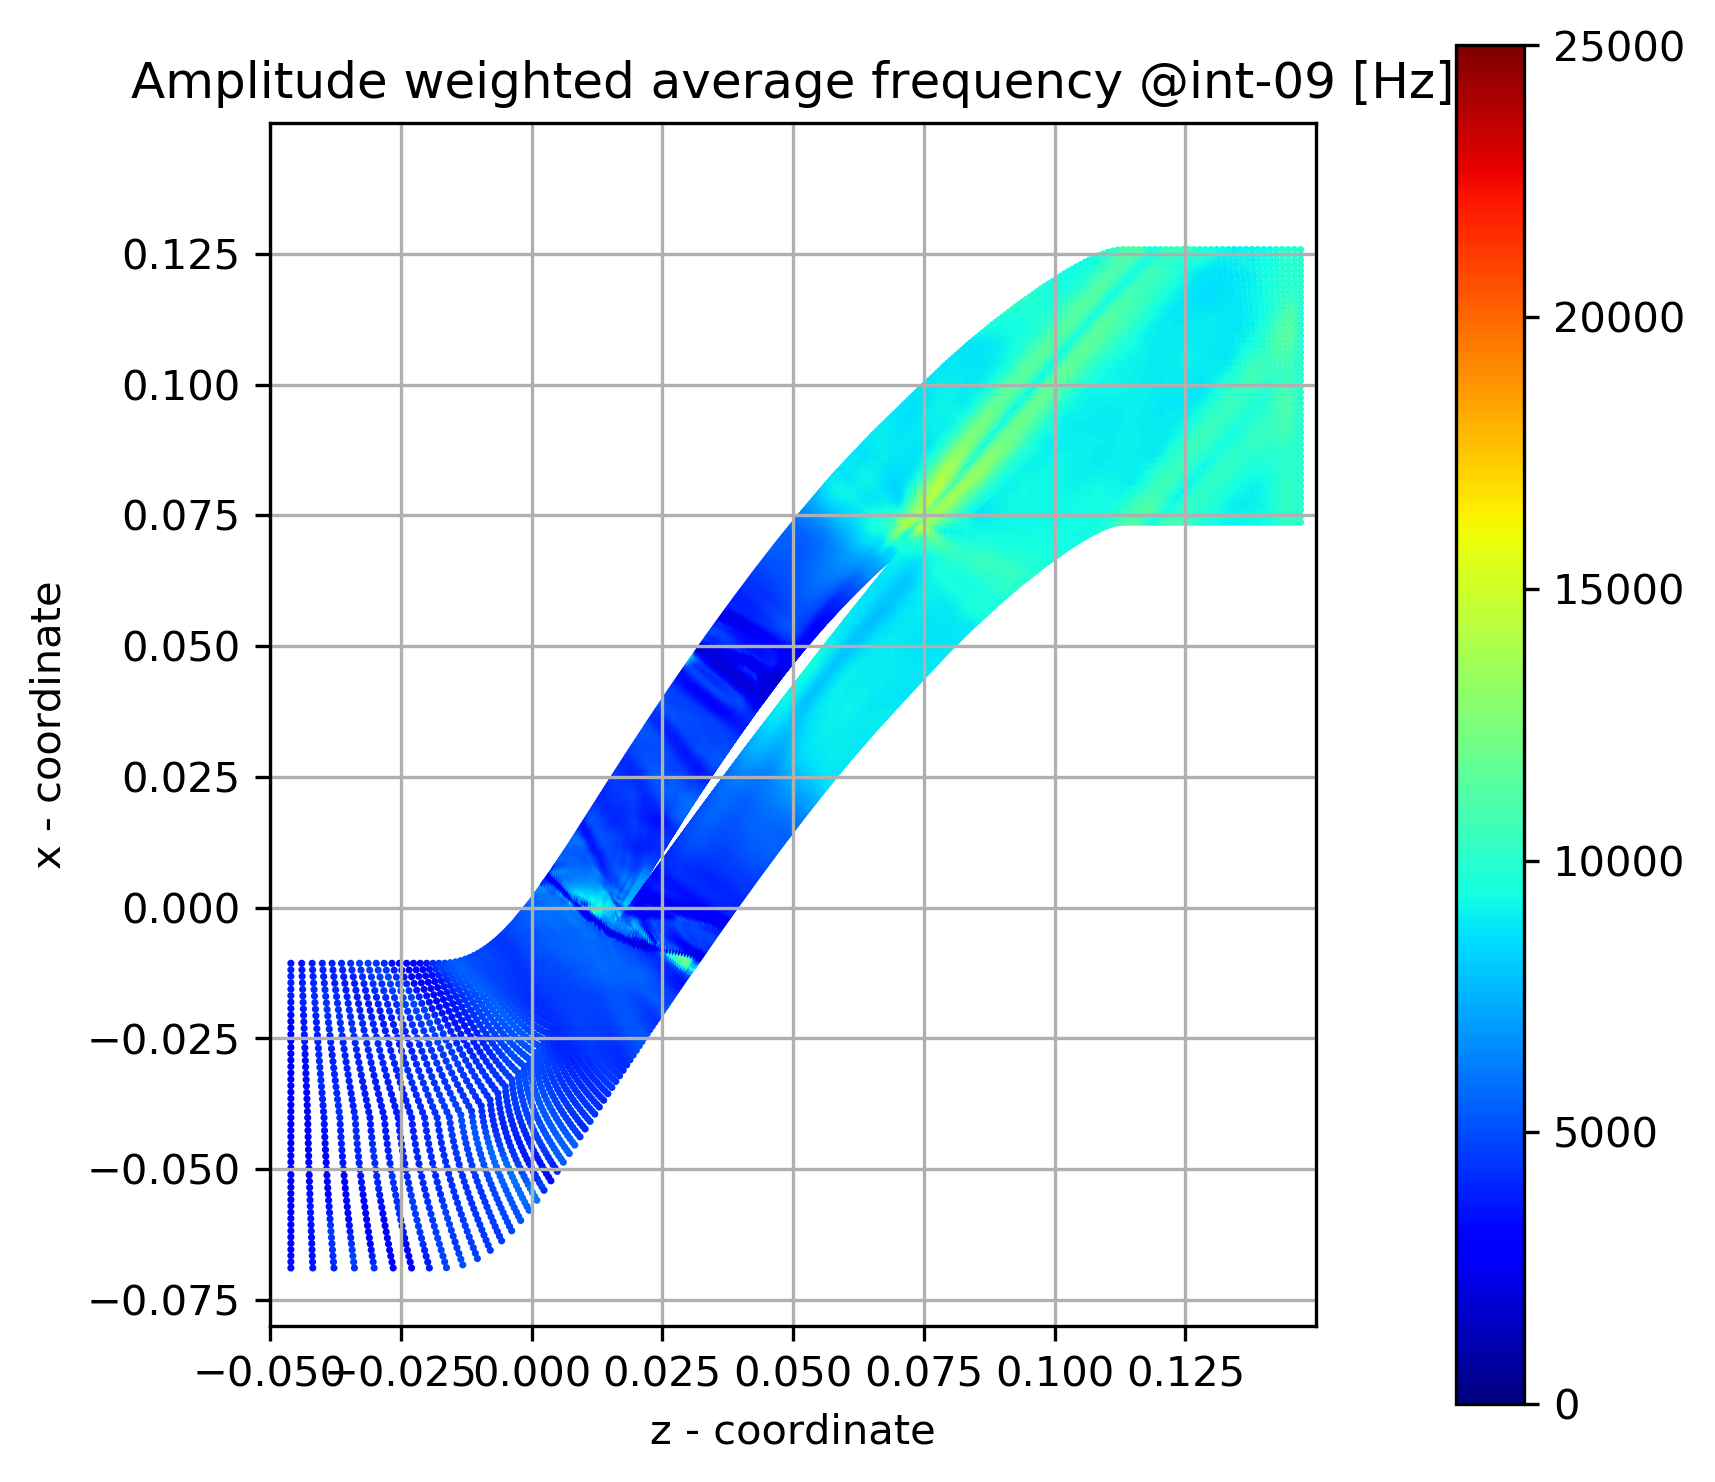
\includegraphics[width=0.75\textwidth]{Figures/int-09-awaf.png}
  \caption{Amplitude weighted average frequency at int-09 mark} \label{int-09-awaf}
\end{figure}
%int-09
\begin{figure}[ht]
  \centering
  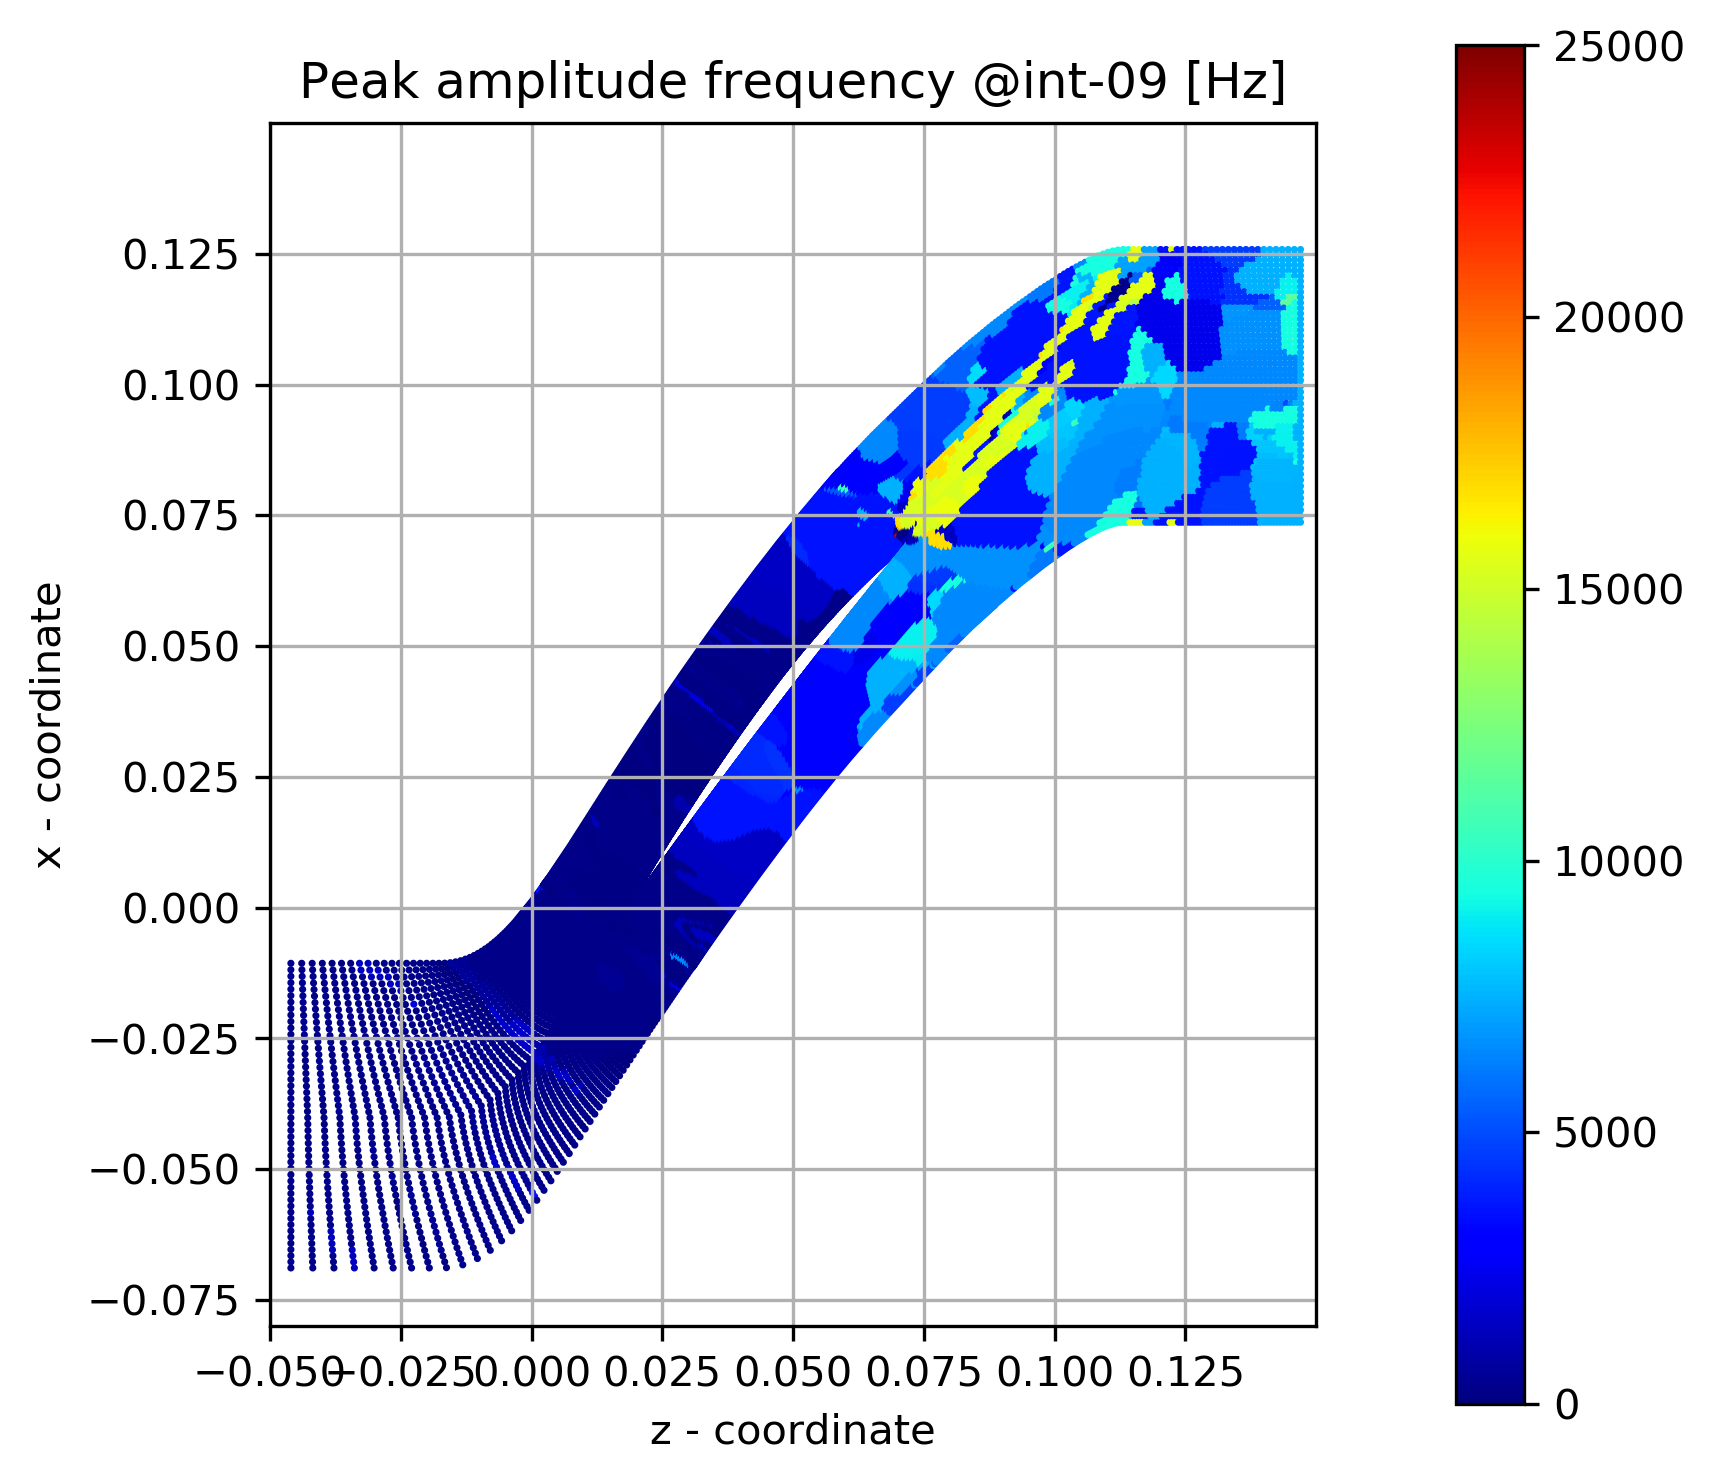
\includegraphics[width=0.75\textwidth]{Figures/int-09-peak-freq.png}
  \caption{Peak amplitude frequency int-09 mark} \label{int-09-peak-freq}
  
  \vspace*{\floatsep}% https://tex.stackexchange.com/q/26521/5764

  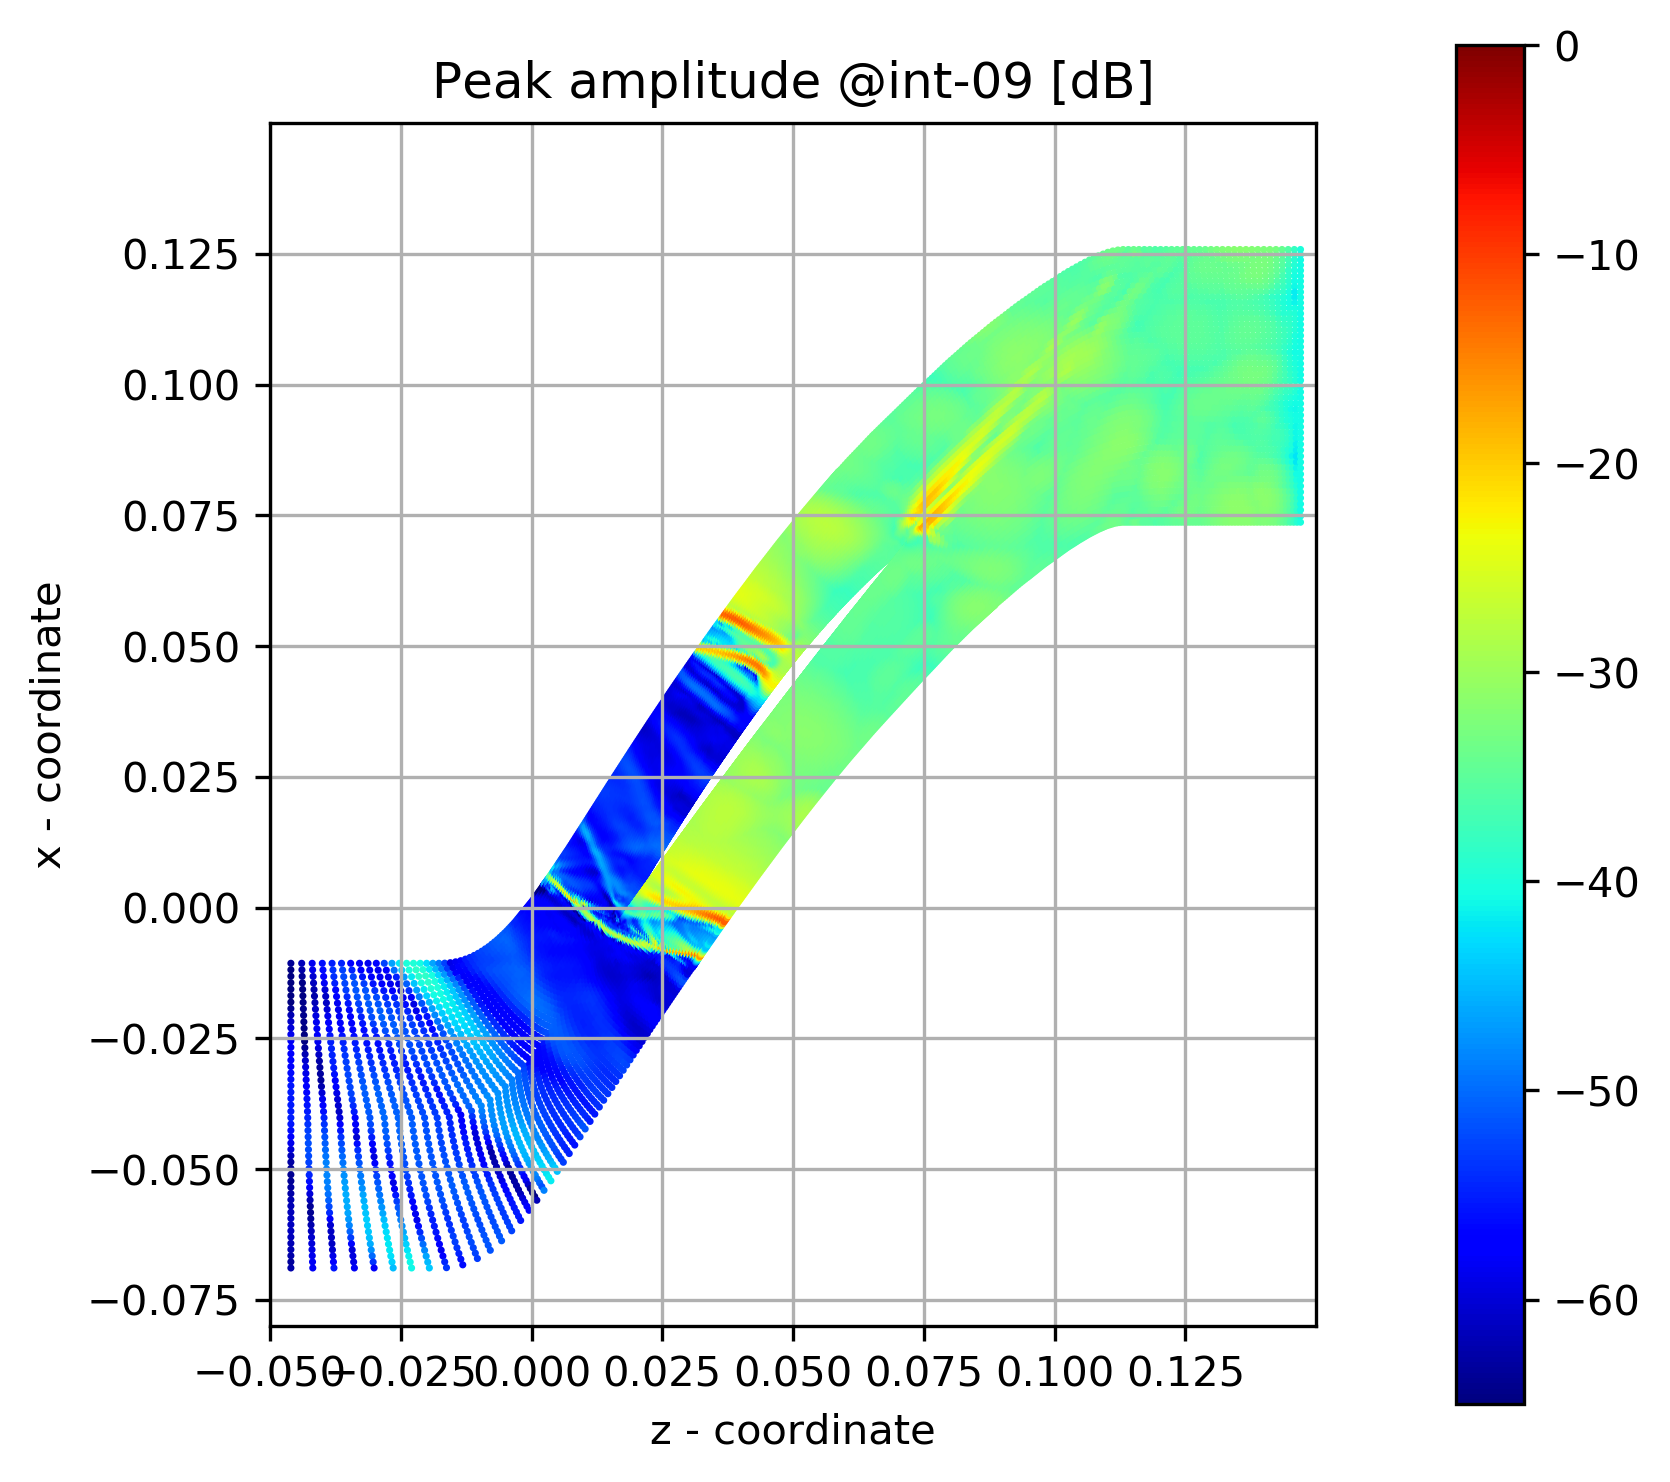
\includegraphics[width=0.75\textwidth]{Figures/int-09-peak-mag.png}
  \caption{Peak magnitude at int-09 mark} \label{int-09-peak-mag}
\end{figure}

%int-10
\begin{figure}[ht]
  \centering
  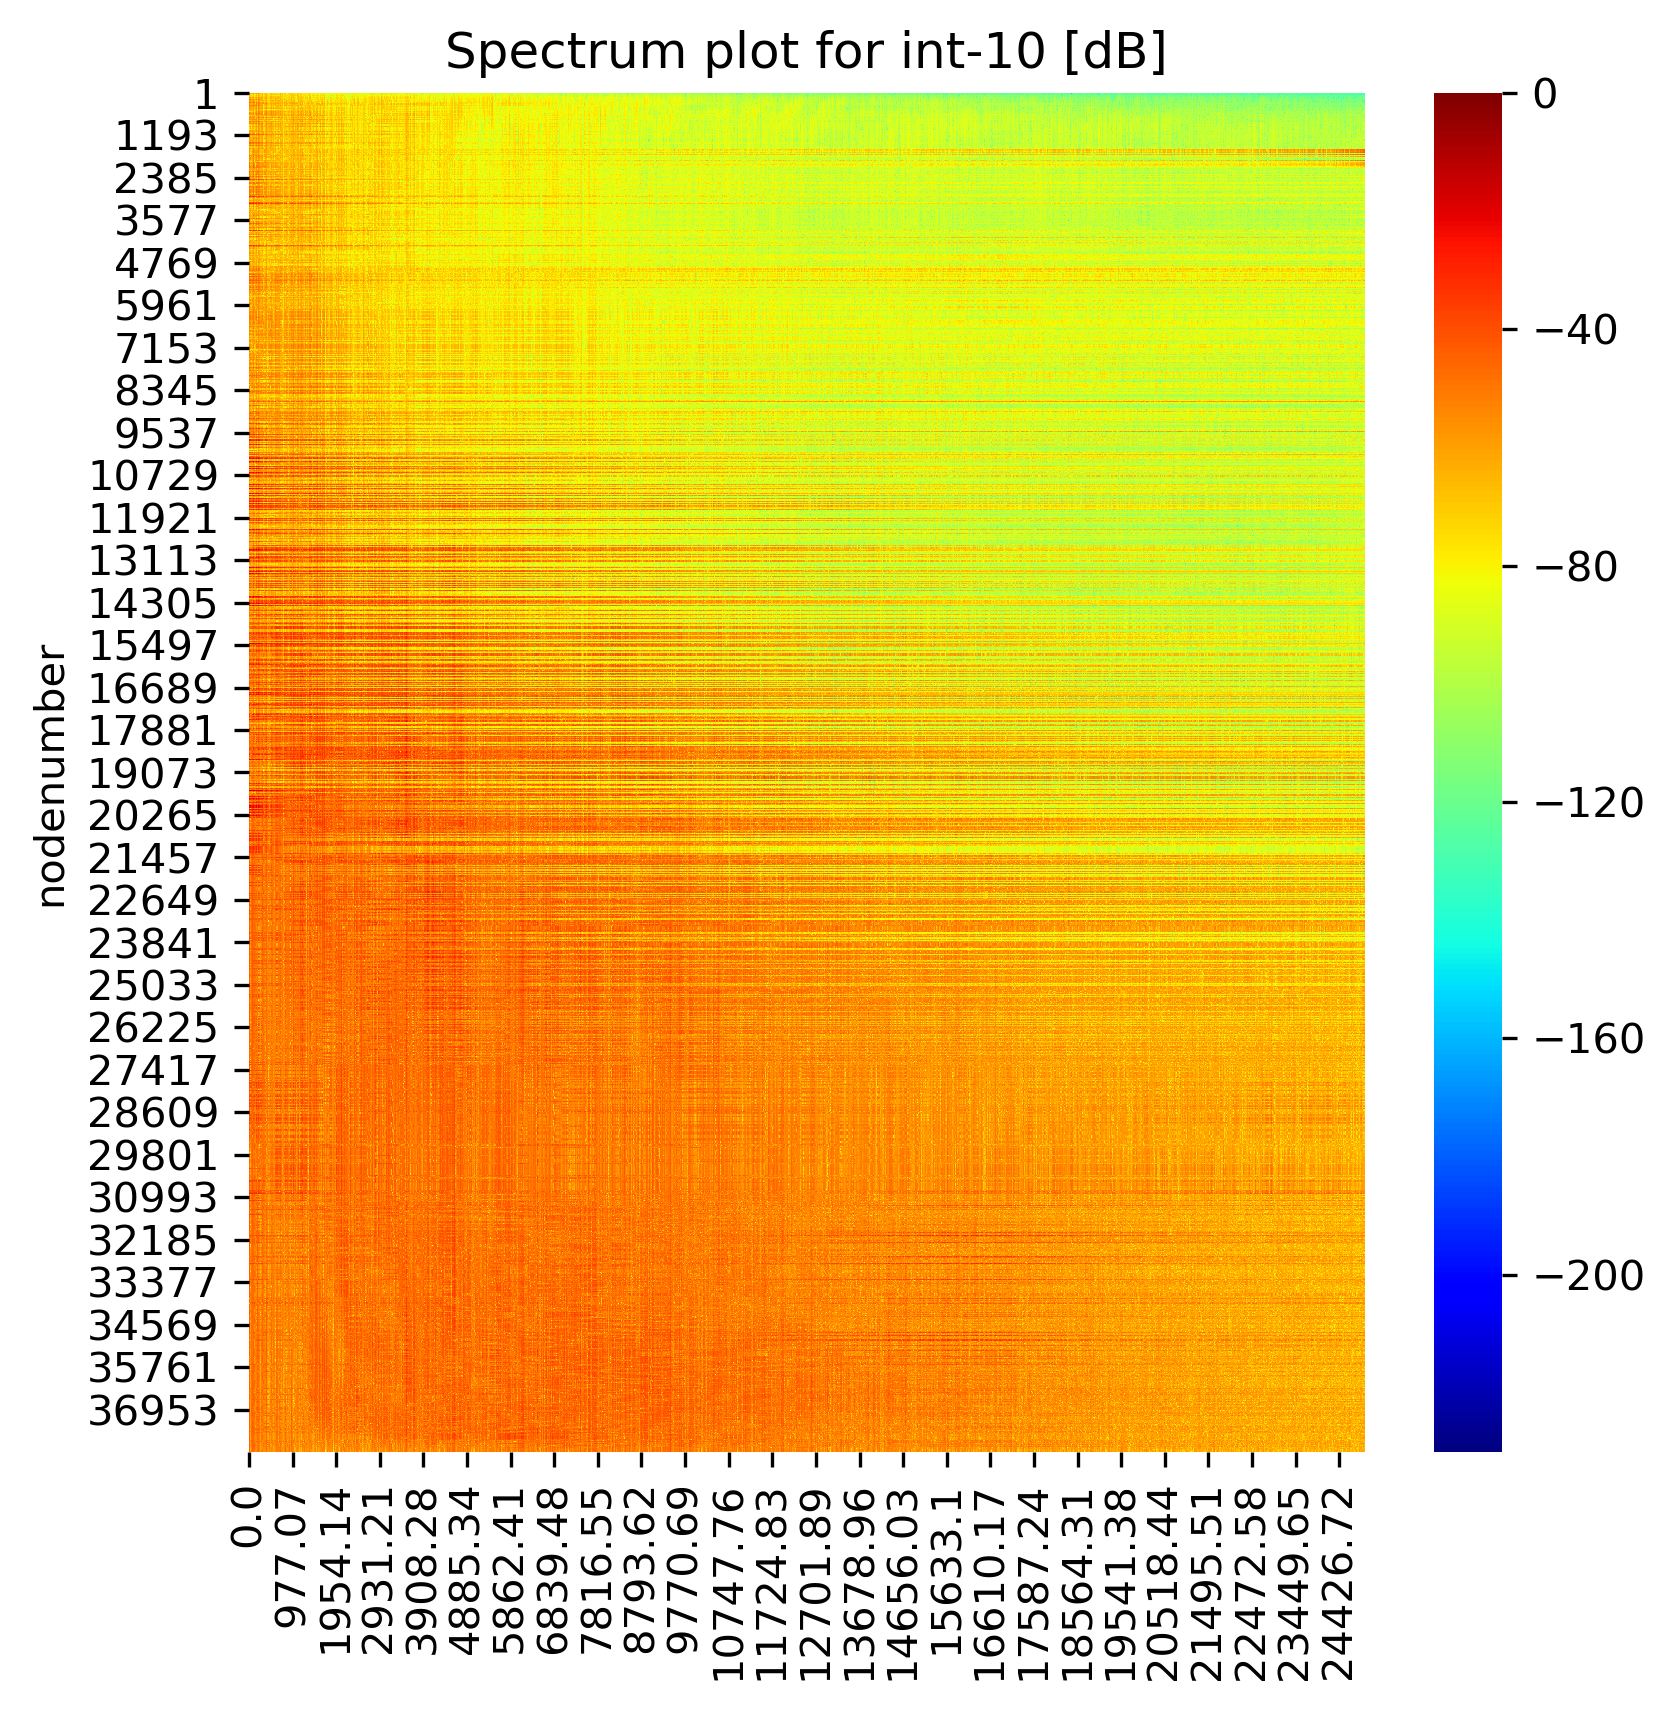
\includegraphics[width=0.75\textwidth]{Figures/int-10_spectrum.png}
  \caption{Spectrum plot at int-10 mark} \label{int-10-spectrum}
  
  \vspace*{\floatsep}% https://tex.stackexchange.com/q/26521/5764

  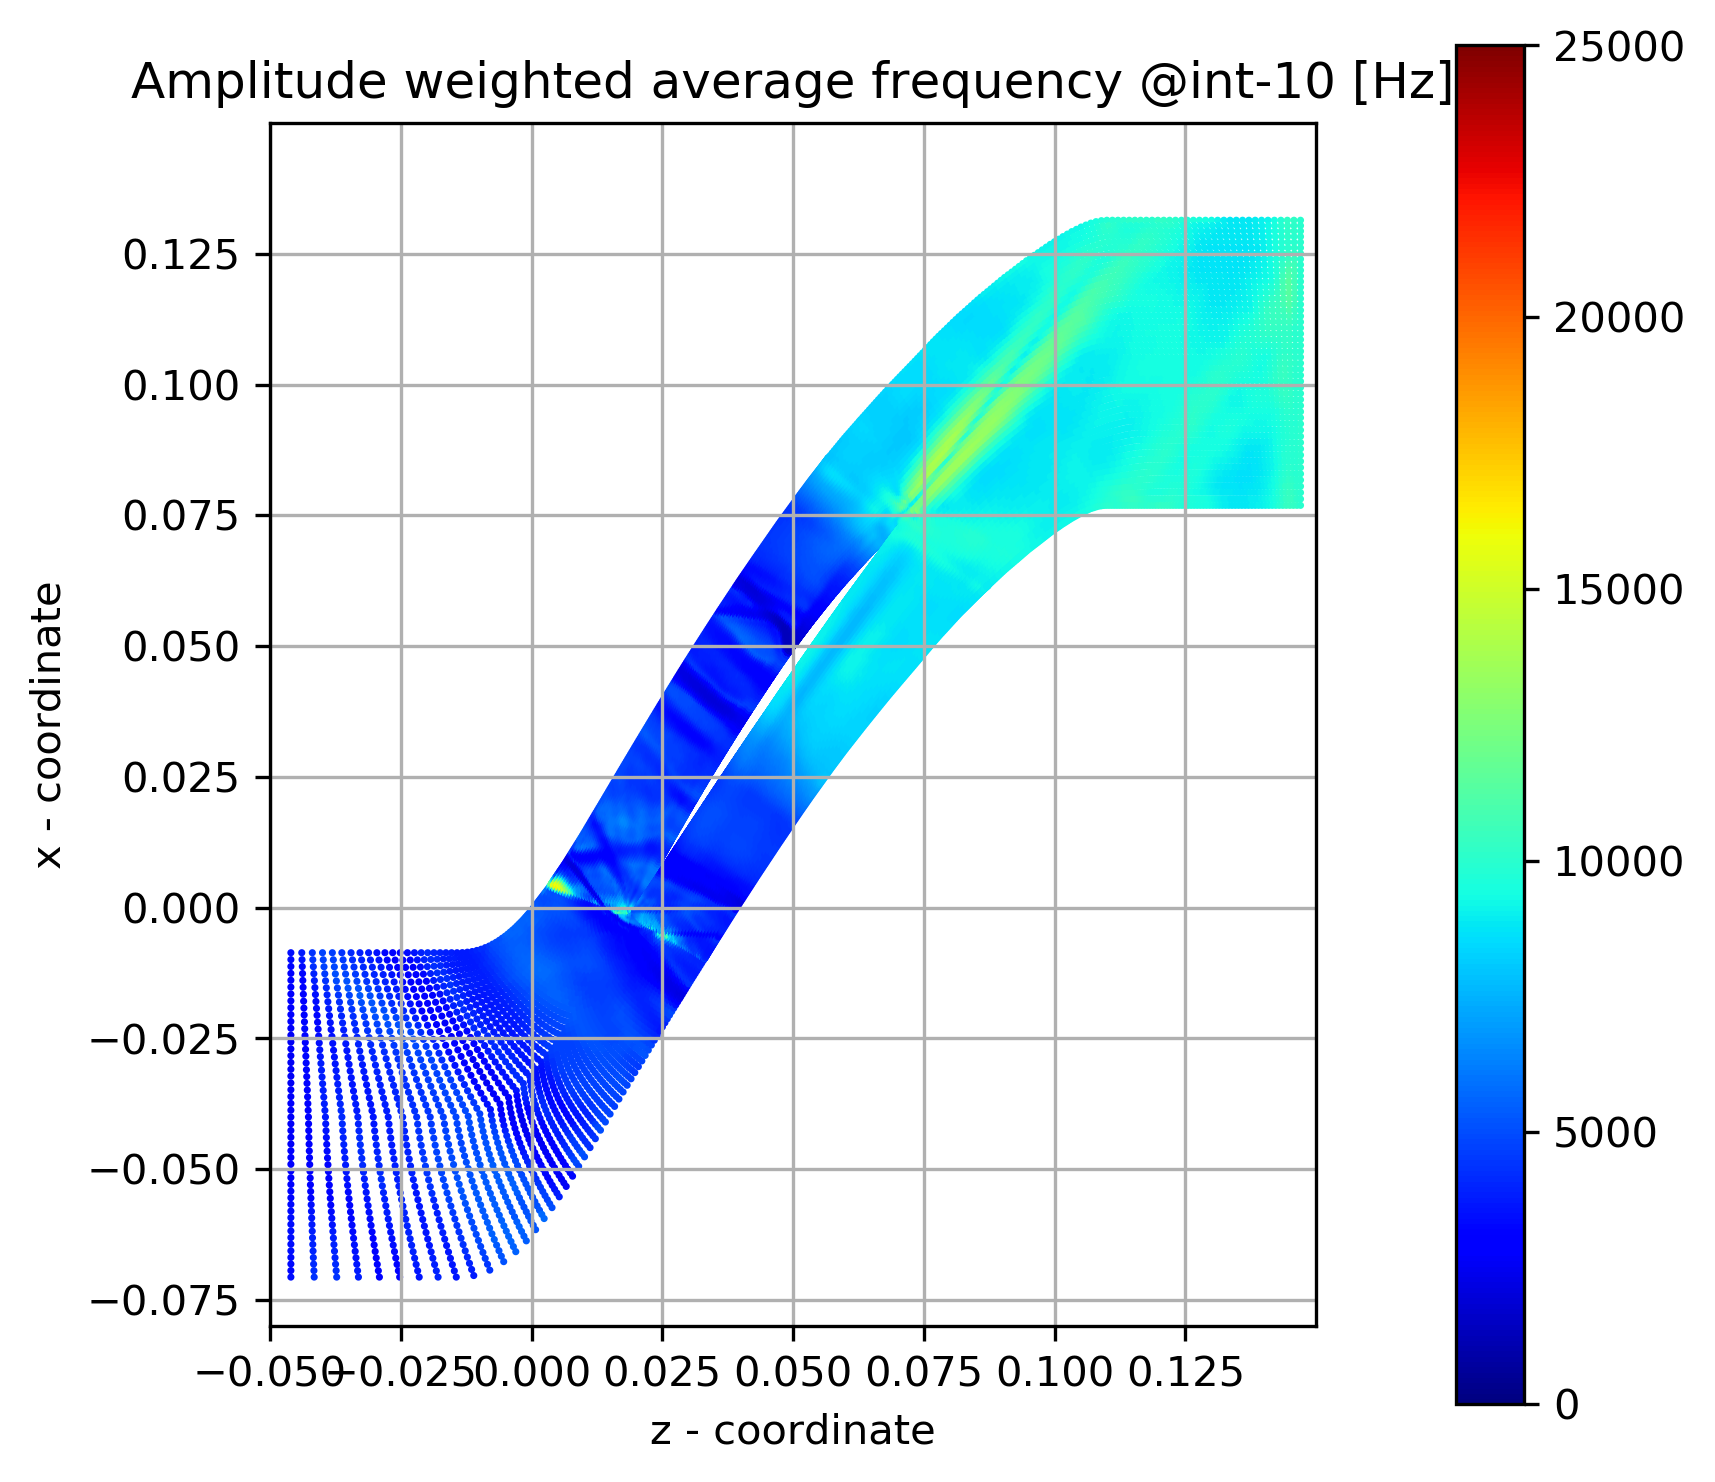
\includegraphics[width=0.75\textwidth]{Figures/int-10-awaf.png}
  \caption{Amplitude weighted average frequency at int-10 mark} \label{int-10-awaf}
\end{figure}
%int-10
\begin{figure}[ht]
  \centering
  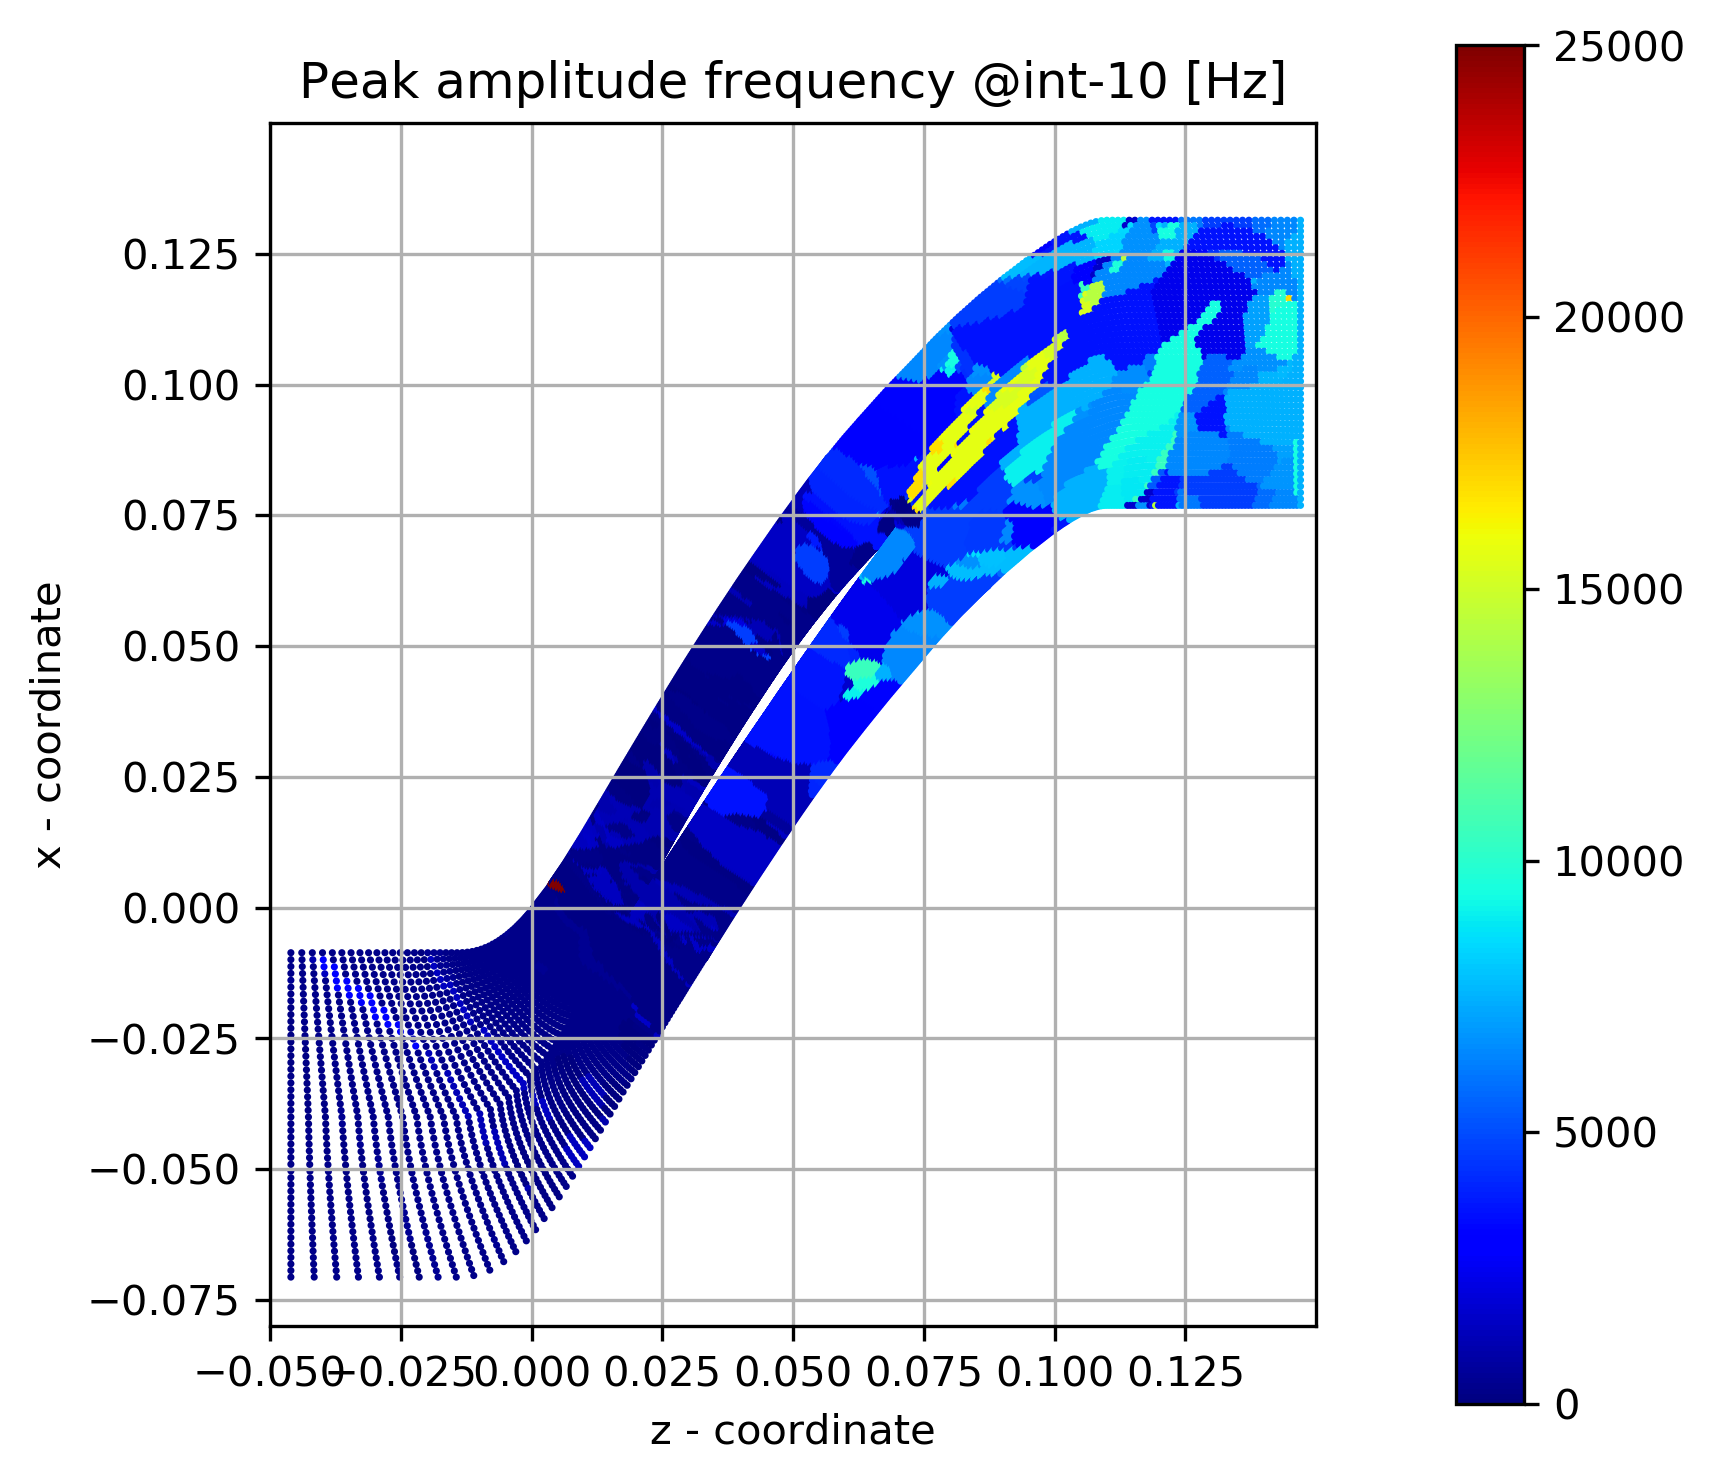
\includegraphics[width=0.75\textwidth]{Figures/int-10-peak-freq.png}
  \caption{Peak amplitude frequency int-10 mark} \label{int-10-peak-freq}
  
  \vspace*{\floatsep}% https://tex.stackexchange.com/q/26521/5764

  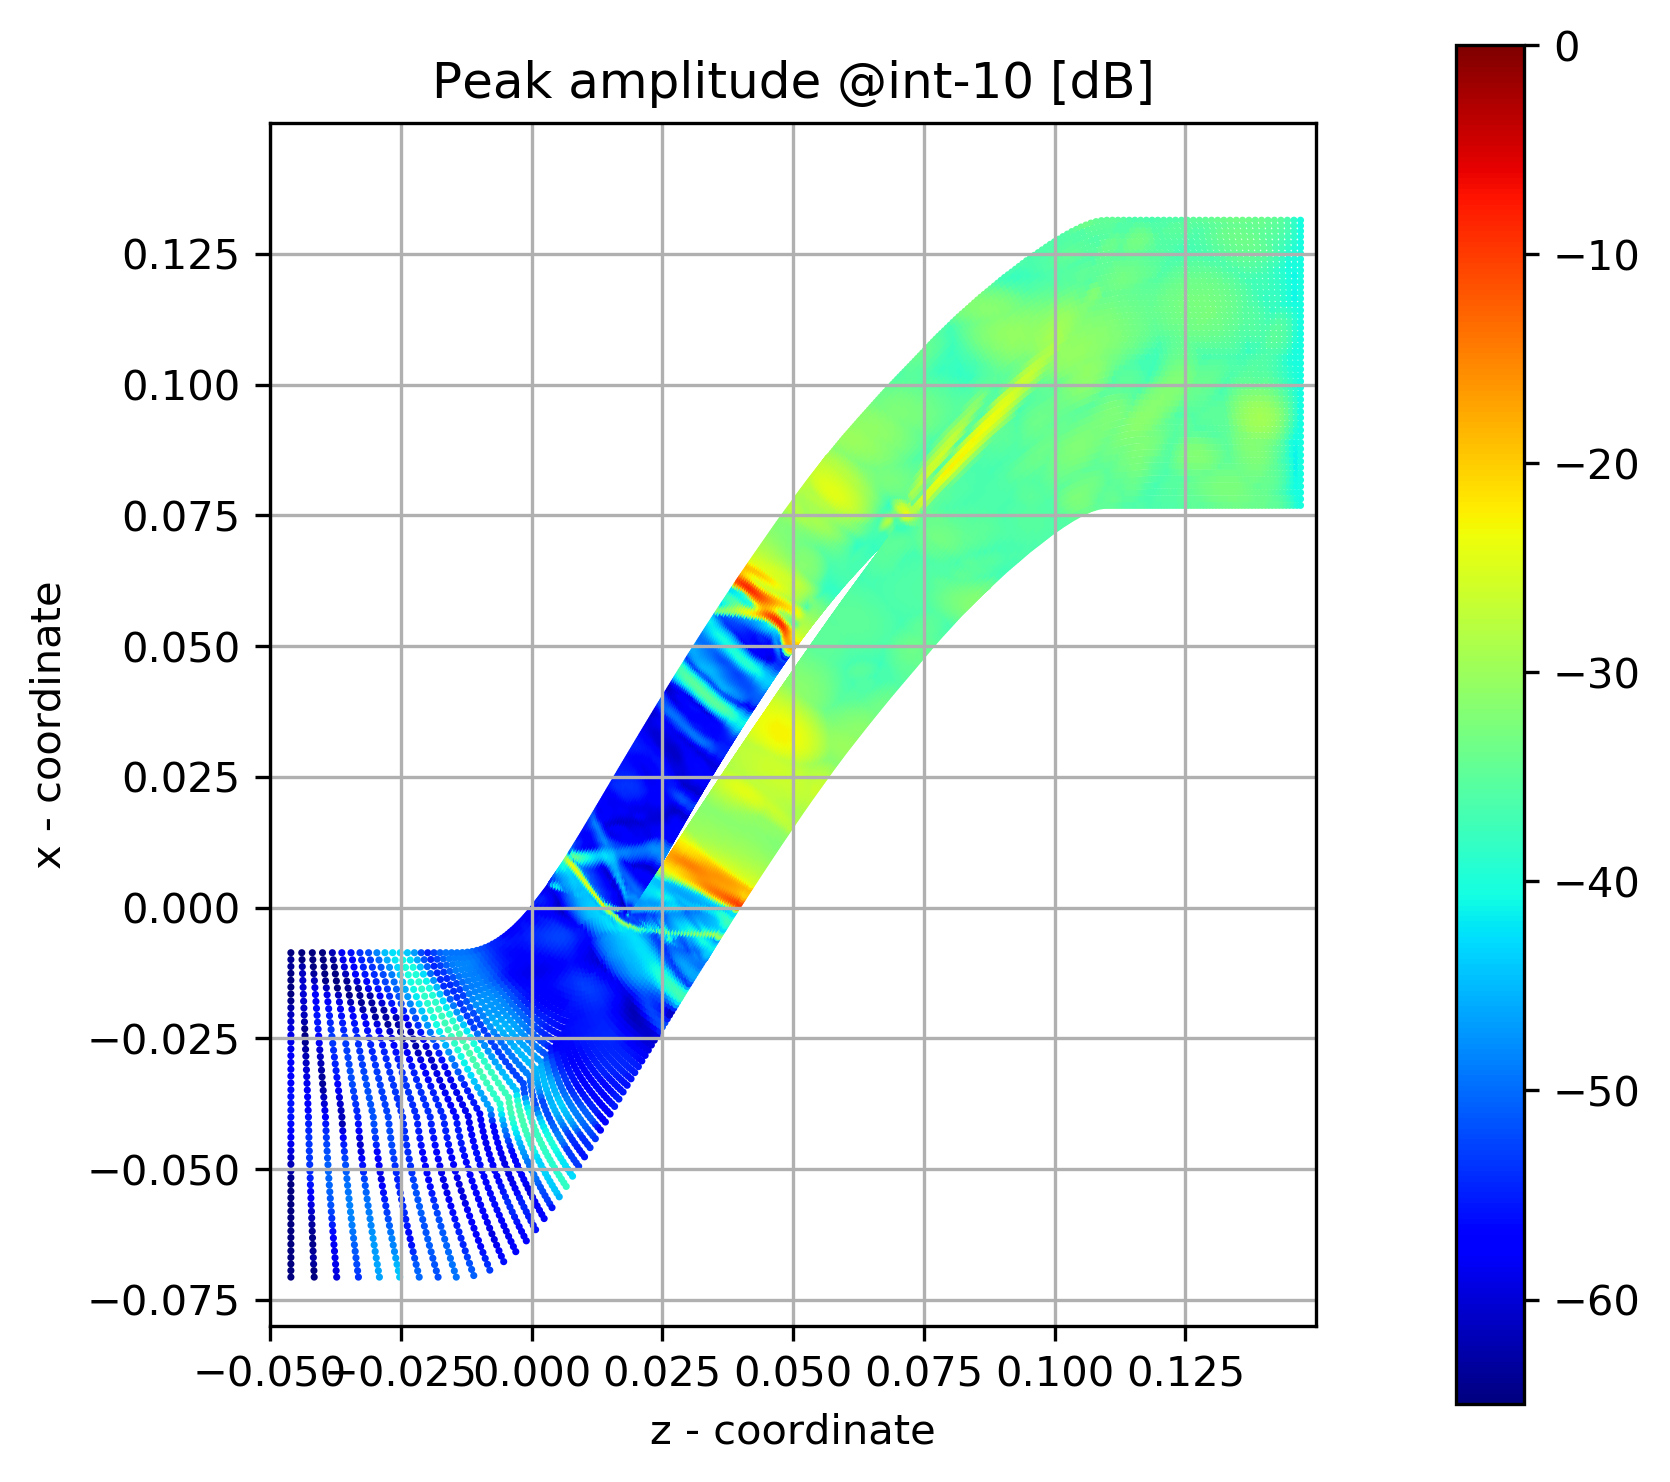
\includegraphics[width=0.75\textwidth]{Figures/int-10-peak-mag.png}
  \caption{Peak magnitude at int-10 mark} \label{int-10-peak-mag}
\end{figure}

%int-11
\begin{figure}[ht]
  \centering
  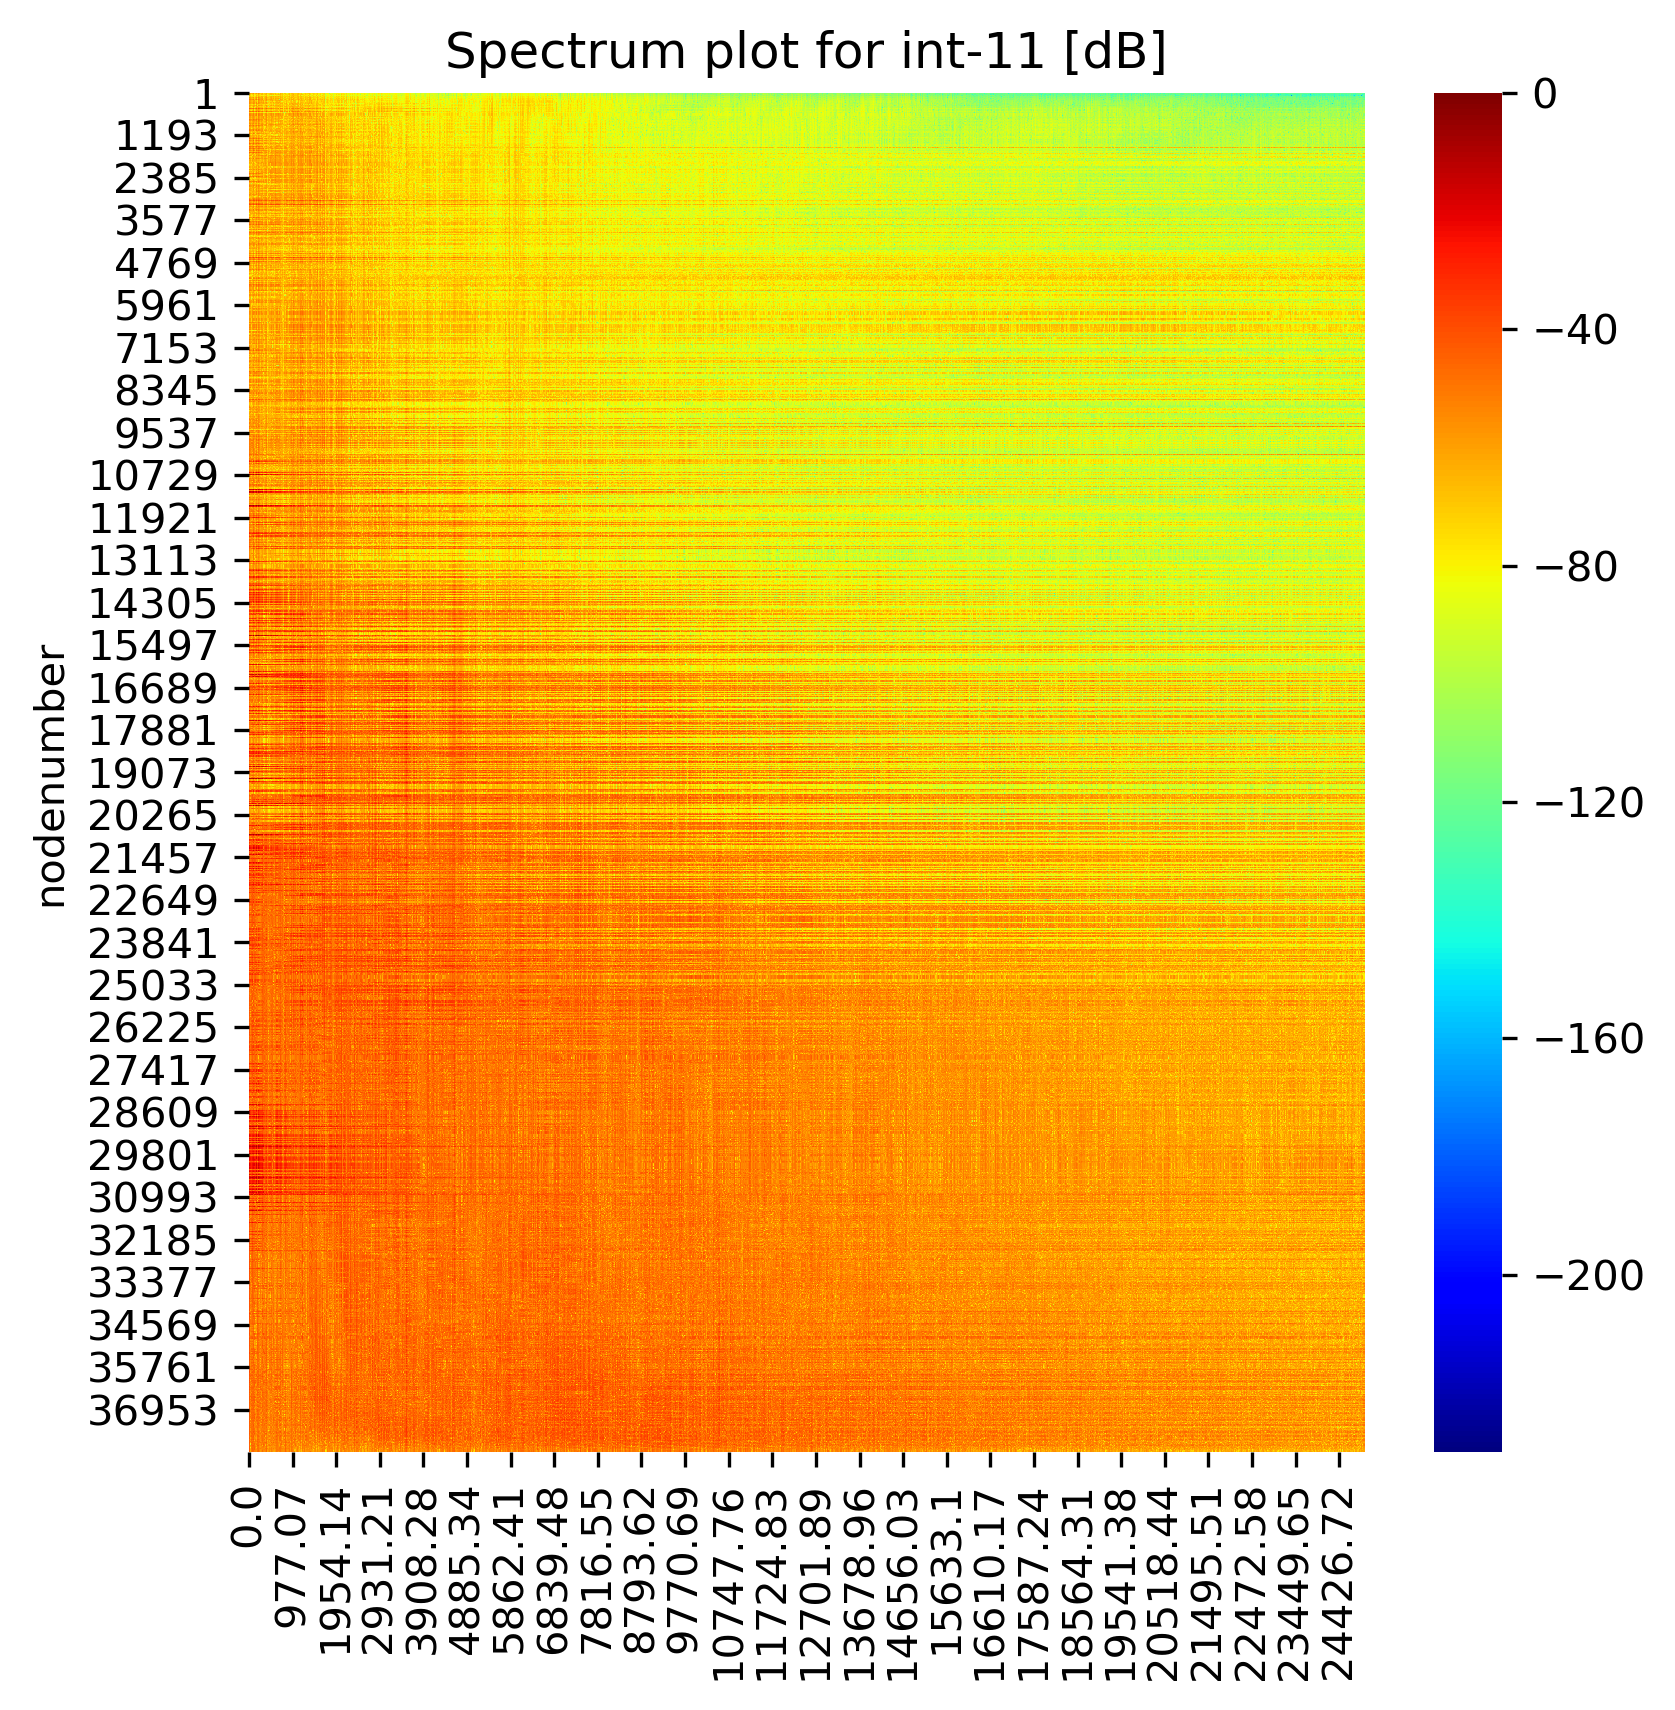
\includegraphics[width=0.75\textwidth]{Figures/int-11_spectrum.png}
  \caption{Spectrum plot at int-11 mark} \label{int-11-spectrum}
  
  \vspace*{\floatsep}% https://tex.stackexchange.com/q/26521/5764

  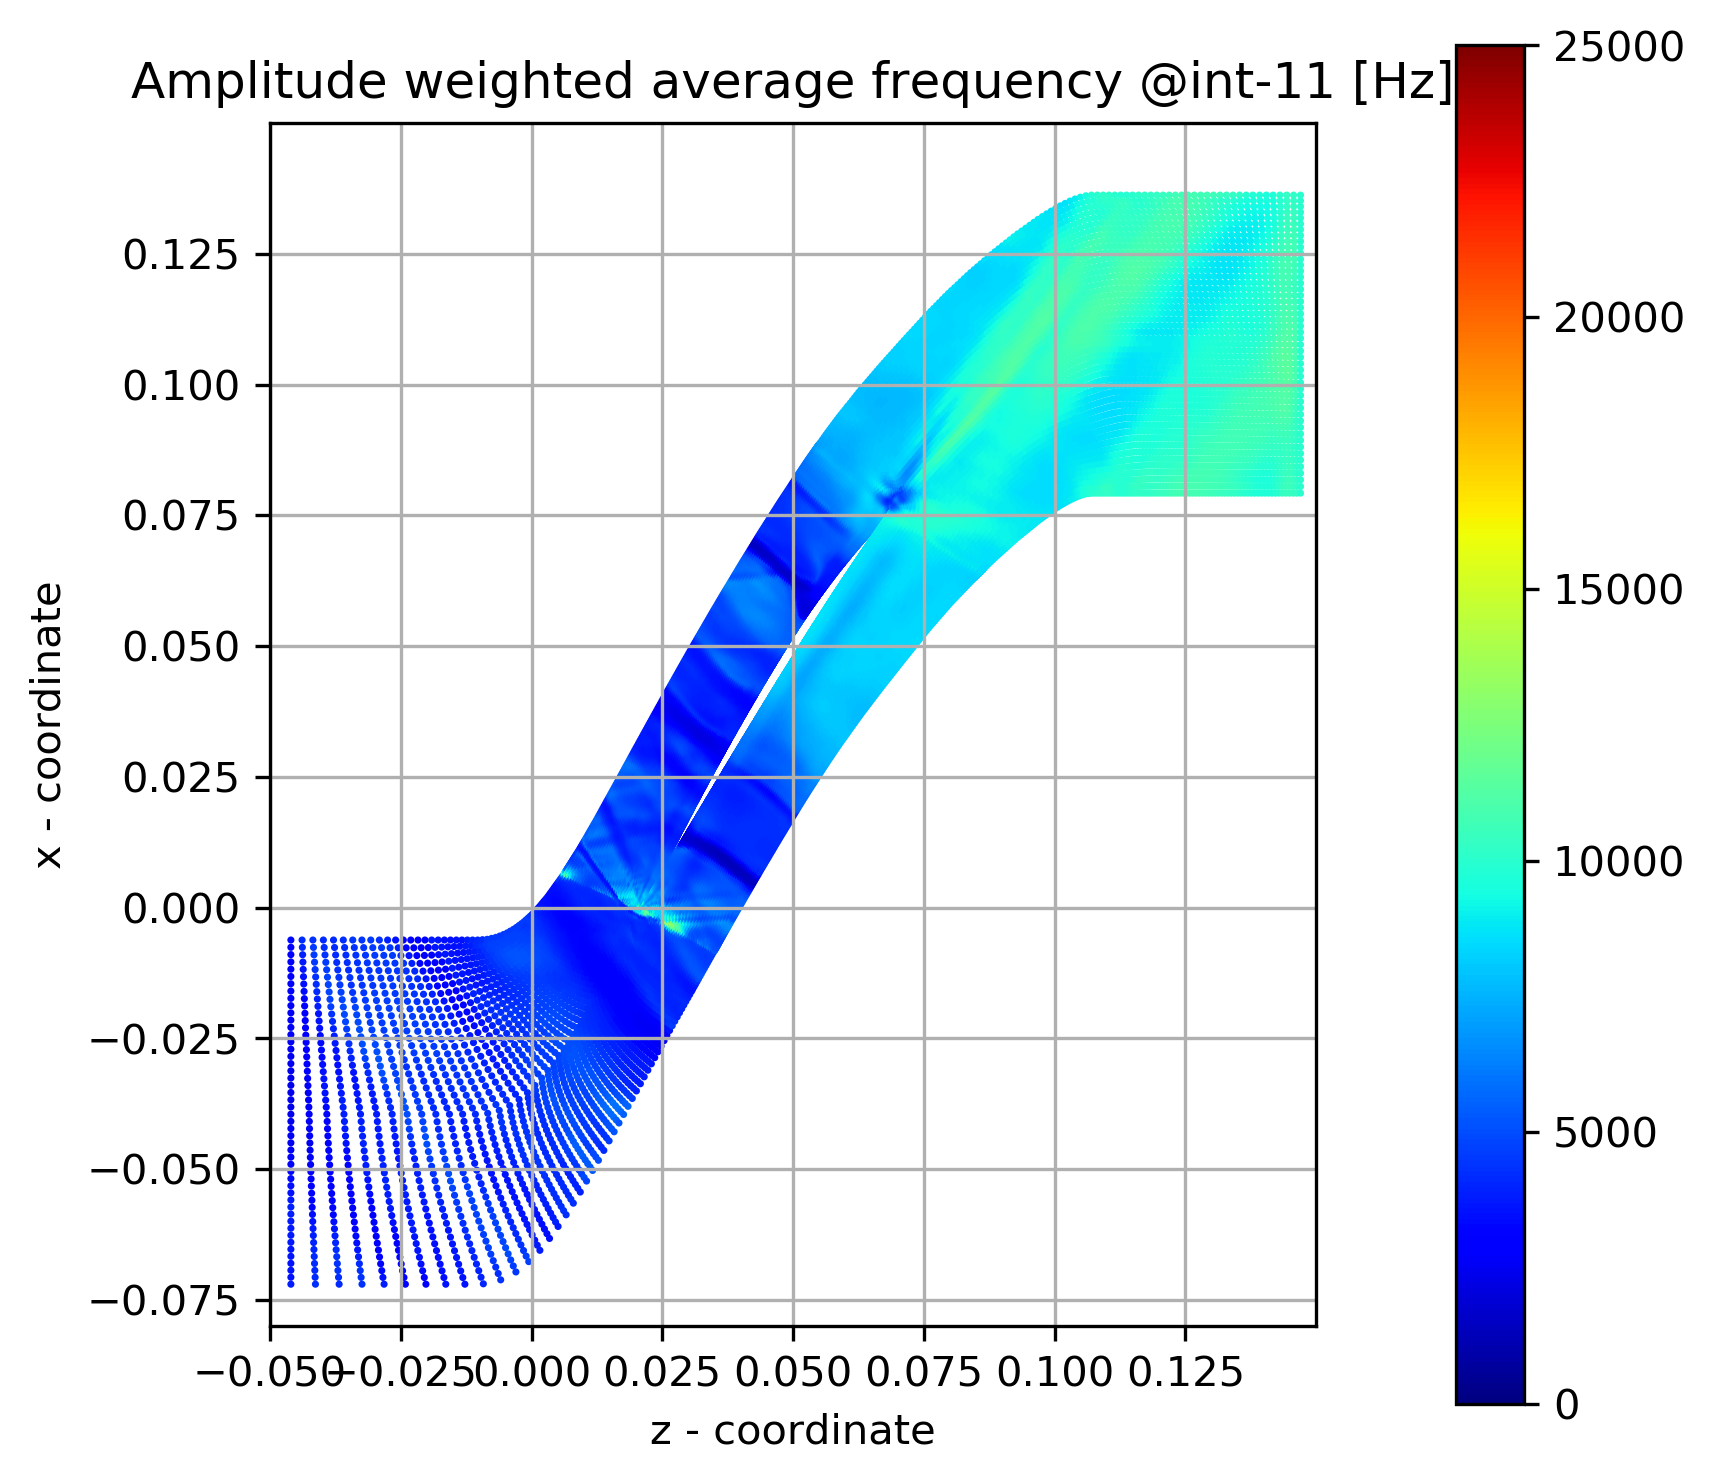
\includegraphics[width=0.75\textwidth]{Figures/int-11-awaf.png}
  \caption{Amplitude weighted average frequency at int-11 mark} \label{int-11-awaf}
\end{figure}
%int-11
\begin{figure}[ht]
  \centering
  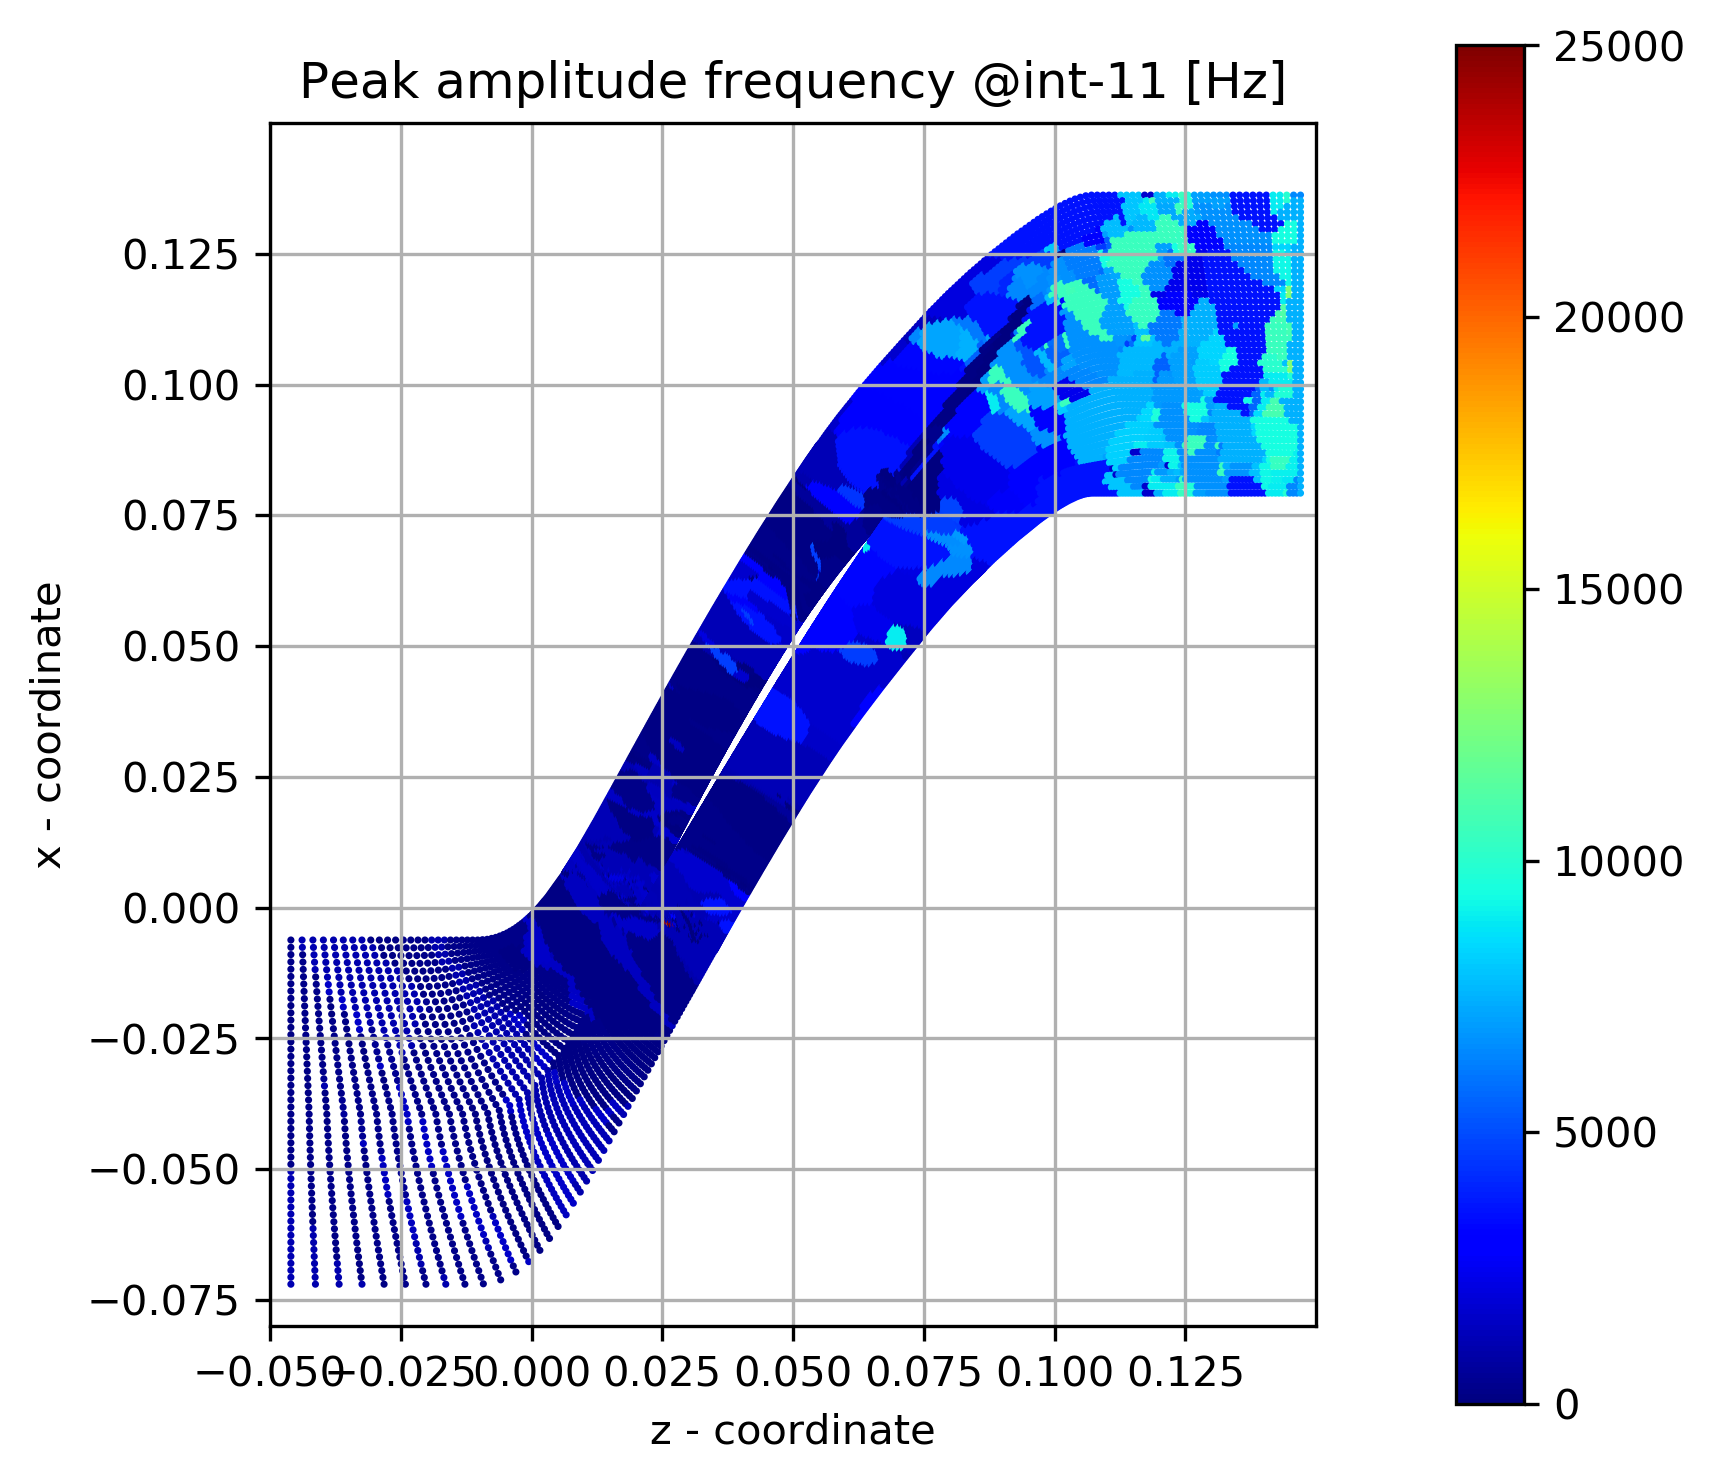
\includegraphics[width=0.75\textwidth]{Figures/int-11-peak-freq.png}
  \caption{Peak amplitude frequency int-11 mark} \label{int-11-peak-freq}
  
  \vspace*{\floatsep}% https://tex.stackexchange.com/q/26521/5764

  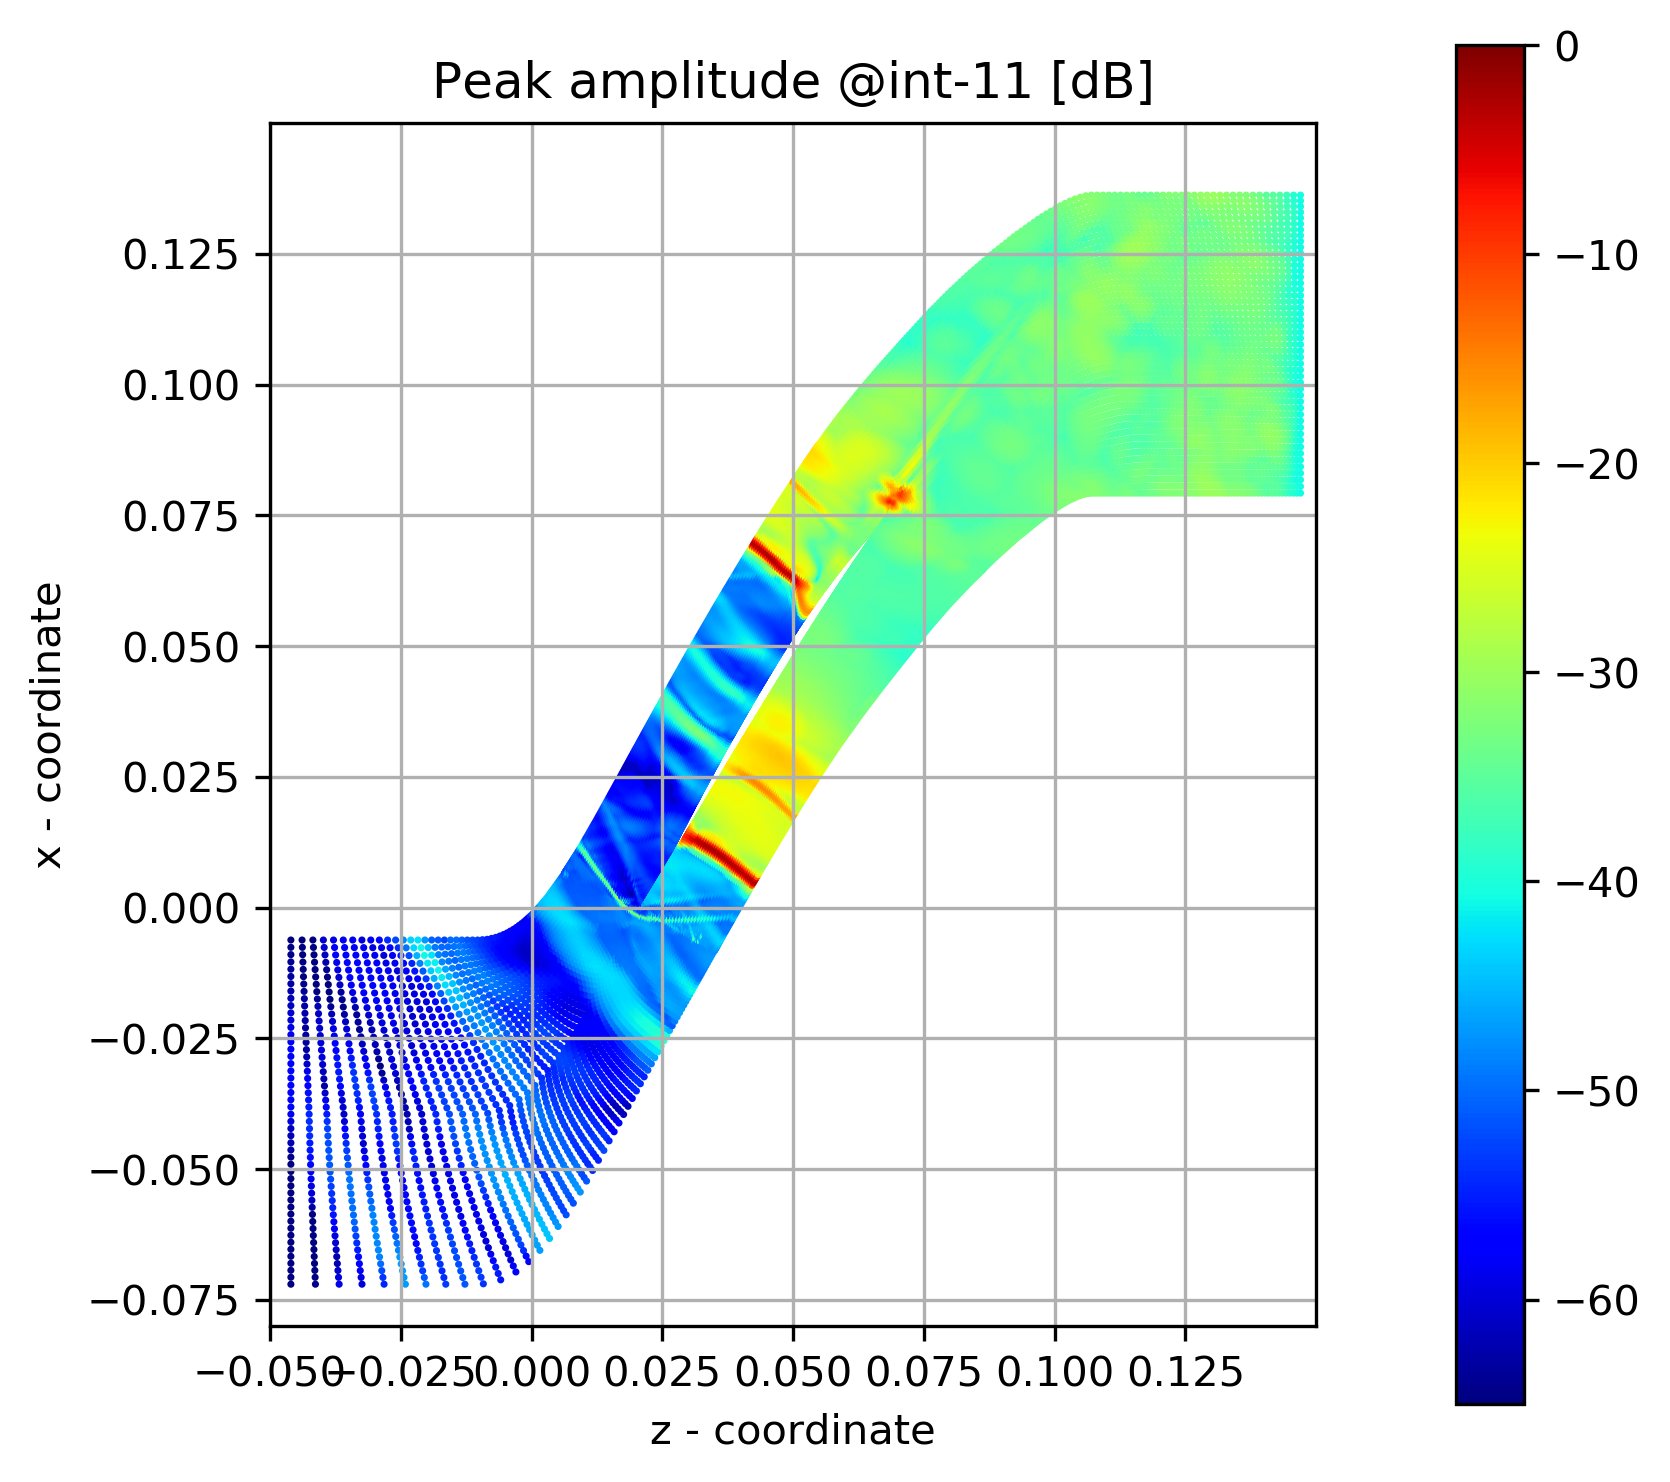
\includegraphics[width=0.75\textwidth]{Figures/int-11-peak-mag.png}
  \caption{Peak magnitude at int-11 mark} \label{int-11-peak-mag}
\end{figure}

%int-12
\begin{figure}[ht]
  \centering
  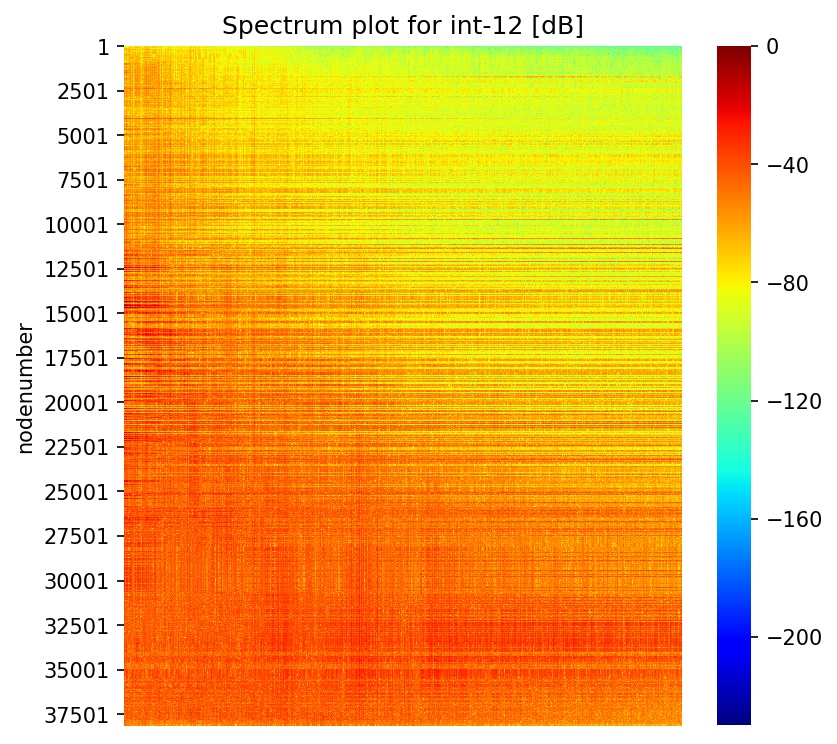
\includegraphics[width=0.75\textwidth]{Figures/int-12_spectrum.png}
  \caption{Spectrum plot at int-12 mark} \label{int-12-spectrum}
  
  \vspace*{\floatsep}% https://tex.stackexchange.com/q/26521/5764

  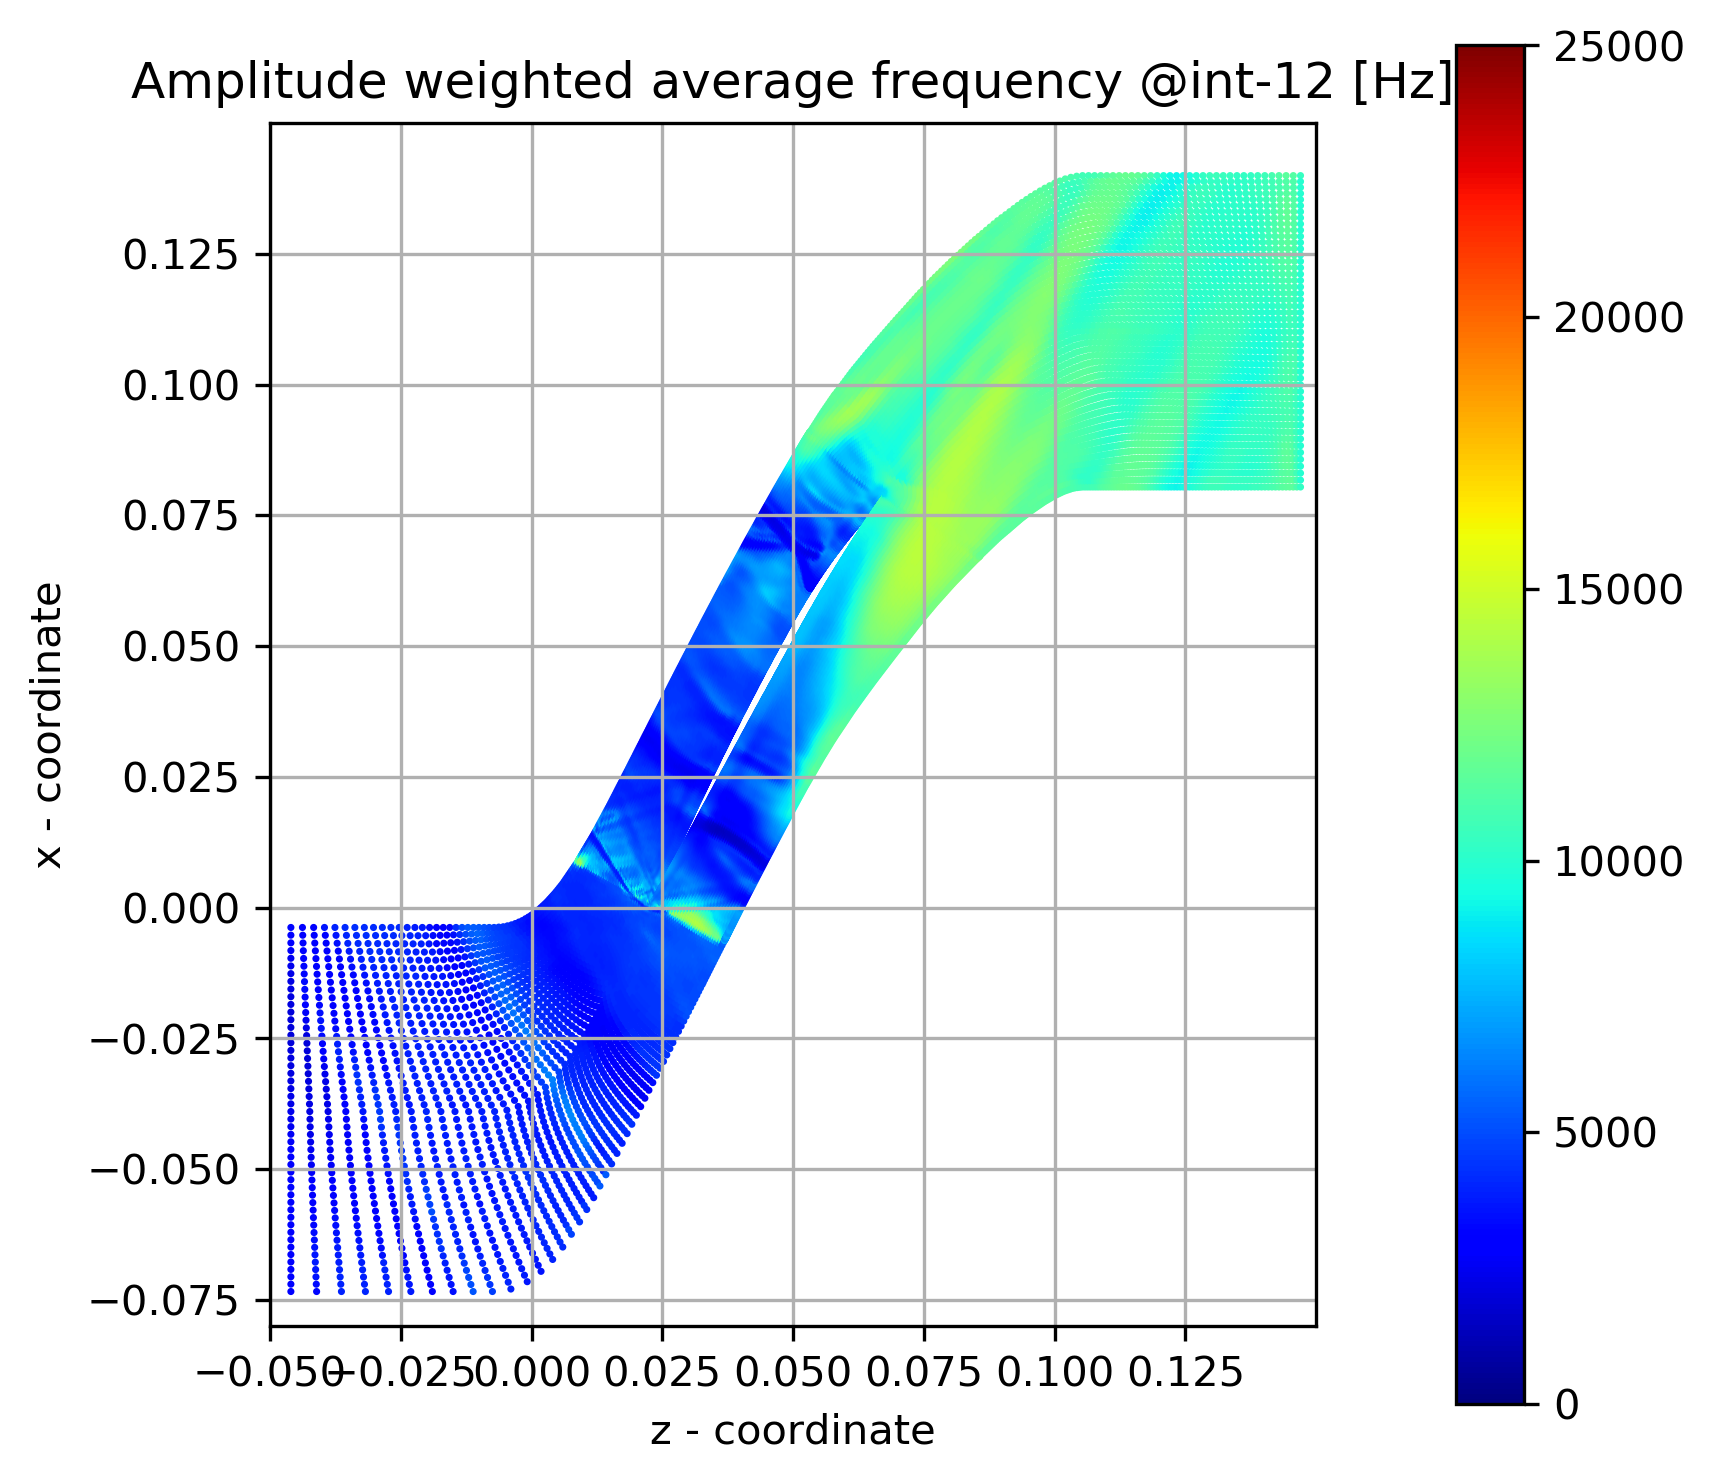
\includegraphics[width=0.75\textwidth]{Figures/int-12-awaf.png}
  \caption{Amplitude weighted average frequency at int-12 mark} \label{int-12-awaf}
\end{figure}
%int-12
\begin{figure}[ht]
  \centering
  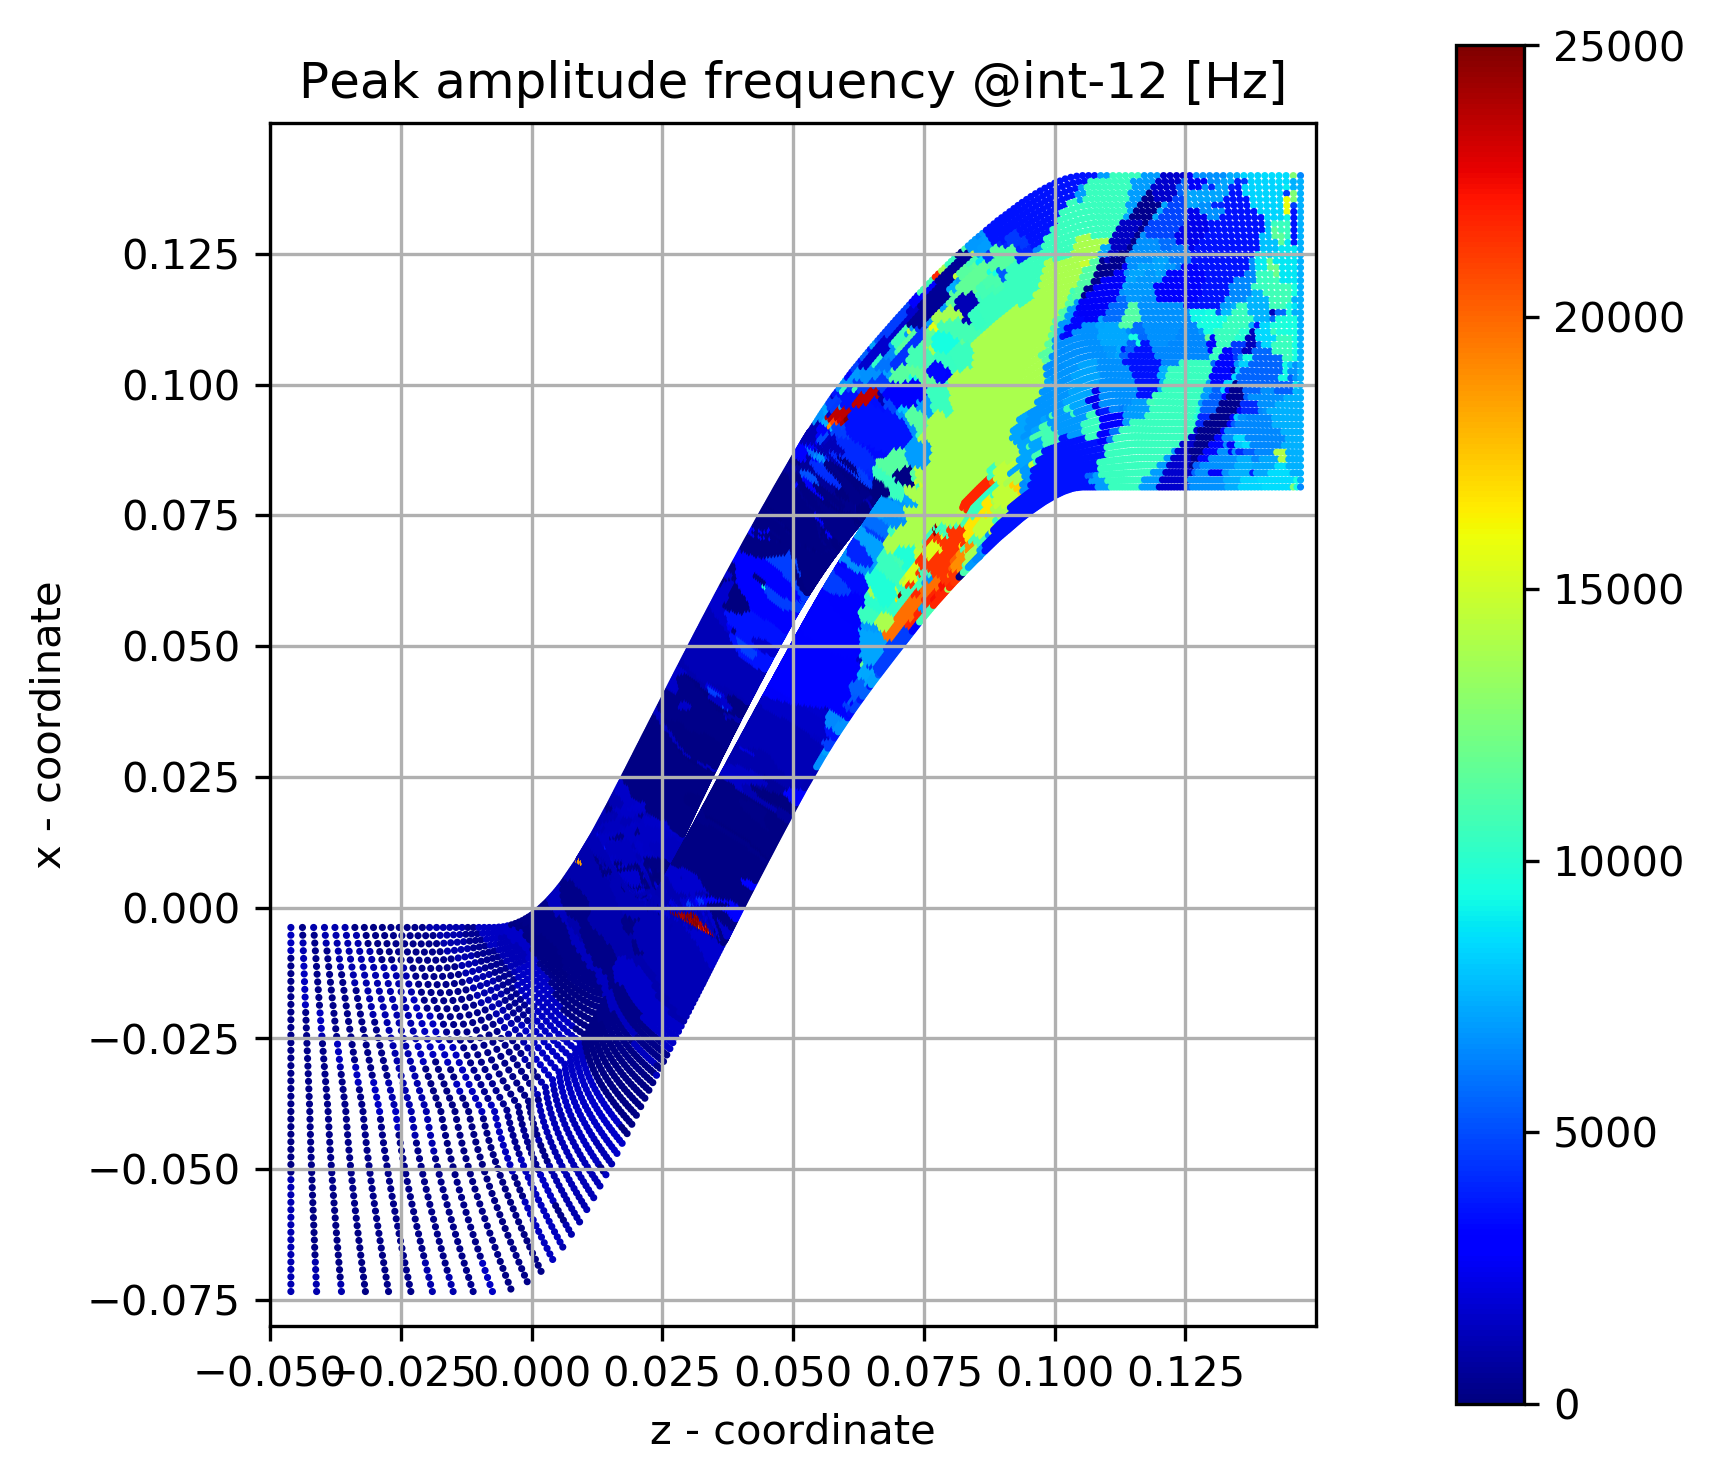
\includegraphics[width=0.75\textwidth]{Figures/int-12-peak-freq.png}
  \caption{Peak amplitude frequency int-12 mark} \label{int-12-peak-freq}
  
  \vspace*{\floatsep}% https://tex.stackexchange.com/q/26521/5764

  \includegraphics[width=0.75\textwidth]{Figures/int-12-peak-mag.png}
  \caption{Peak magnitude at int-12 mark} \label{int-12-peak-mag}
\end{figure}

%int-tip
\begin{figure}[ht]
  \centering
  \includegraphics[width=0.75\textwidth]{Figures/int-tip_spectrum.png}
  \caption{Spectrum plot at int-tip mark} \label{int-tip-spectrum}
  
  \vspace*{\floatsep}% https://tex.stackexchange.com/q/26521/5764

  \includegraphics[width=0.75\textwidth]{Figures/int-tip-awaf.png}
  \caption{Amplitude weighted average frequency at int-tip mark} \label{int-tip-awaf}
\end{figure}
%int-tip
\begin{figure}[ht]
  \centering
  \includegraphics[width=0.75\textwidth]{Figures/int-tip-peak-freq.png}
  \caption{Peak amplitude frequency int-tip mark} \label{int-tip-peak-freq}
  
  \vspace*{\floatsep}% https://tex.stackexchange.com/q/26521/5764

  \includegraphics[width=0.75\textwidth]{Figures/int-tip-peak-mag.png}
  \caption{Peak magnitude at int-tip mark} \label{int-tip-peak-mag}
\end{figure}